\documentclass{article}

\usepackage{hyperref}
\usepackage[utf8]{inputenc}
\usepackage{amsfonts}
\usepackage{amsmath}
\usepackage{amssymb}
\usepackage{dsfont} % for using \mathds{1} characteristic function
\usepackage{tikz}
\usepackage{bbm}
\usepackage{relsize}
\usepackage{pgfplots}
\pgfplotsset{compat=1.18}
\usepackage{scalerel}
\usepackage{wrapfig}
\usepackage[T1]{fontenc}       % change font encoding to T1
\usepackage[framed,numbered]{matlab-prettifier}


%toglie lo spazio dato dal doppio invio
\setlength{\parindent}{0cm} 

%distanza dal numero di pagina
\setlength{\footskip}{1.3cm}


\usepackage[
	left=2.5cm, % inner
	right=2.5cm, % outer
	top=2.3cm,
	bottom=2.8cm,
	%showframe,
	]{geometry}







\renewcommand{\contentsname}{Indice}



\title{Modelli e Metodi delle EDP}
\author{Simone Paloschi}
\date{INGMTM \ \ A.A. 2022/2023}
\linespread{1.5}

\DeclareRobustCommand{\Chi}{{\mathpalette\irchi\relax}}
\newcommand{\irchi}[2]{\raisebox{\depth}{$#1\chi$}} % inner command, used by \Chi


\newcommand{\EE}{\mathbb E}
\newcommand{\NN}{\mathbb N}
\newcommand{\PP}{\mathbb P}
\newcommand{\R}{\mathbb R}
\newcommand{\ZZ}{\mathbb Z}

\newcommand{\Ac}{\mathcal A}
\newcommand{\Bc}{\mathcal B}
\newcommand{\Cc}{\mathcal C}
\newcommand{\Ec}{\mathcal E}
\newcommand{\Fc}{\mathcal F}
\newcommand{\Gc}{\mathcal G}
\newcommand{\Hc}{\mathcal H}
\newcommand{\Lc}{\mathcal L}
\newcommand{\Nc}{\mathcal N}
\newcommand{\Pc}{\mathcal P}
\newcommand{\Uc}{\mathcal U}
\newcommand{\Vc}{\mathcal V}
\newcommand{\Oc}{\mathcal O}
\newcommand{\Tau}{\mathcal T}

\usepackage{esvect}

%%%%% shortcuts

\newcommand{\eps}{\varepsilon}
\renewcommand{\phi}{\varphi}



%displaystyle frazione e integrale
\renewcommand{\frac}{\dfrac}

\let \INT \int 
\renewcommand{\int}{\displaystyle\INT}


\newcommand{\ind}{\perp \!\!\! \perp} % indipendenza

%displaystyle sommatoria e prod
\newcommand{\Sum}[2]{\sum\limits_{#1}^{#2}} 

\newcommand{\Prod}[2]{\prod\limits_{#1}^{#2}}



%displaystyle parentesi

\renewcommand{\O}{\left(}
\newcommand{\C}{\right)}

\newcommand{\OO}{\left[}
\newcommand{\CC}{\right]}

\newcommand{\OOO}{\left\{}
\newcommand{\CCC}{\right\}}


%matrice indicatrice
\newcommand{\II}{\mathds{1}}

%insieme vuoto
\renewcommand{\empty}{\emptyset}


\renewcommand{\hat}[1]{\widehat{#1}}
\renewcommand{\tilde}[1]{\widetilde{#1}}


 \newcommand{\Asterisk}{\mathop{\scalebox{1.5}{\raisebox{-0.2ex}{$\ast$}}}} %for big * 





%per farmi aprire le parentesi da \vv
%\renewcommand{\vv}{\vv}





%%%%%%%%%%%%%%%%%%%%%%%%%%%%%%
%AMBIENTI TEOREMI
%%%%%%%%%%%%%%%%%%%%%%%%%%%%%%



\usepackage{amsthm}
\definecolor{Green}{RGB}{0,210,100}
\definecolor{Black}{RGB}{0,0,0}
\definecolor{Blue}{RGB}{0,120,245}
\newtheoremstyle{DEFstyle} % Theorem style name
{0pt}% Space above
{0pt}% Space below
{\normalfont}% Body font
{}% Indent amount
{\bf\scshape}% Theorem head font --- {\small\bf}
{.\\}% Punctuation after theorem head
{0em}% Space after theorem head
{\small\thmname{#1}% Theorem text (e.g. Theorem 2.1)
%{\small\thmname{#1}% Theorem text (e.g. Theorem)
\thmnote{:\nobreakspace\normalfont\bfseries \nobreakspace#3}}% Optional theorem note



\newtheoremstyle{DIMstyle} % Theorem style name
{0pt}% Space above
{0pt}% Space below
{\normalfont}% Body font
{}% Indent amount
{\bf\scshape}% Theorem head font --- {\small\bf}
{\\}% Punctuation after theorem head
{0em}% Space after theorem head
{\small\thmname{#1}.% Theorem text (e.g. Theorem 2.1)
%{\small\thmname{#1}% Theorem text (e.g. Theorem)
\thmnote{\nobreakspace\normalfont\nobreakspace(#3)}}% Optional theorem note

\newtheoremstyle{RIPstyle} % Theorem style name
{0pt}% Space above
{0pt}% Space below
{\normalfont}% Body font
{}% Indent amount
{\bf\scshape}% Theorem head font --- {\small\bf}
{\\}% Punctuation after theorem head
{0em}% Space after theorem head
{\small\thmname{#1}:% Theorem text (e.g. Theorem 2.1)
%{\small\thmname{#1}% Theorem text (e.g. Theorem)
\thmnote{\nobreakspace\normalfont\nobreakspace#3}}% Optional theorem note



\newtheoremstyle{CORstyle} % Theorem style name
{0pt}% Space above
{0pt}% Space below
{\normalfont}% Body font
{}% Indent amount
{\bf\scshape}% Theorem head font --- {\small\bf}
{\\}% Punctuation after theorem head
{0em}% Space after theorem head
{\small\thmname{#1}\,\thmnumber{#2}:% Theorem text (e.g. Theorem 2.1)
%{\small\thmname{#1}% Theorem text (e.g. Theorem)
\thmnote{\nobreakspace\normalfont \nobreakspace#3}}% Optional theorem note



\theoremstyle{DEFstyle}
\newtheorem* {theoremT}{Definizione}
\newtheorem* {theoremT1}{Teorema}
\theoremstyle{DIMstyle}
\newtheorem* {theoremT2}{Dim}
\theoremstyle{RIPstyle}
\newtheorem* {theoremT3}{Ripasso}

\theoremstyle{CORstyle}
\newtheorem{theoremT4}{Corollario}

%per cambiare il numero che appare a 6 serve \setcounter{theoremT4}{5}


\RequirePackage[framemethod=default]{mdframed} % Required for creating the theorem, definition, exercise and corollary boxes
% green box
\newmdenv[skipabove=7pt,
skipbelow=7pt,
rightline=false,
leftline=true,
topline=false,
bottomline=false,
linecolor=Green,
backgroundcolor=green!0,
innerleftmargin=5pt,
innerrightmargin=5pt,
innertopmargin=5pt,
leftmargin=0cm,
rightmargin=0cm,
linewidth=2pt,
innerbottommargin=5pt]{gBox}


\newmdenv[skipabove=7pt,
skipbelow=7pt,
rightline=false,
leftline=true,
topline=false,
bottomline=false,
linecolor=Blue,
backgroundcolor=green!0,
innerleftmargin=5pt,
innerrightmargin=5pt,
innertopmargin=5pt,
leftmargin=0cm,
rightmargin=0cm,
linewidth=2pt,
innerbottommargin=5pt]{bBox}


\newmdenv[skipabove=7pt,
skipbelow=20pt,
rightline=false,
leftline=true,
topline=false,
bottomline=false,
linecolor=Black,
backgroundcolor=green!0,
innerleftmargin=5pt,
innerrightmargin=5pt,
innertopmargin=3pt,
leftmargin=0cm,
rightmargin=0cm,
linewidth=0.5pt,
innerbottommargin=5pt]{dimBox}


\newmdenv[skipabove=7pt,
skipbelow=20pt,
rightline=false,
leftline=true,
topline=false,
bottomline=false,
linecolor=Black,
backgroundcolor=green!0,
innerleftmargin=10pt,
innerrightmargin=5pt,
innertopmargin=3pt,
leftmargin=0cm,
rightmargin=0cm,
linewidth=0.5pt,
innerbottommargin=17pt]{ripBox}


\newenvironment{defi}{\begin{gBox}\begin{theoremT}}{\end{theoremT}\end{gBox}}
\newenvironment{teo}{\begin{bBox}\begin{theoremT1}}{\end{theoremT1}\end{bBox}}
\newenvironment{Dim}{\begin{dimBox}\begin{theoremT2}}{\phantom{}\hfill$\qed$\end{theoremT2} \end{dimBox} }
\newenvironment{RIP}{\begin{ripBox}\begin{theoremT3}}{\end{theoremT3}\end{ripBox}}
\newenvironment{cor}{\begin{bBox}\begin{theoremT4}}{\end{theoremT4}\end{bBox}}


%%%%%%%%%%%%%%%%%%%%%%%%%%%%%%
%FIGURA CENTRALE
%%%%%%%%%%%%%%%%%%%%%%%%%%%%%%

\usepackage{caption}\captionsetup{belowskip=12pt,aboveskip=4pt}

\graphicspath{ {./images/} }

\usepackage{placeins} % The placeins package gives the command \FloatBarrier, which will make sure any floats will be put in before this point
\usepackage{flafter}  % The flafter package ensures that floats don't appear until after they appear in the code.

\usepackage{graphicx}
\usepackage{float}

%chiamata:   \fg[ "caption" ]{0.5}{figure.jpeg}
%senza caption non viene \fg{0.5}{figure.jpeg}
\newcommand{\fg}[3][\relax]{%
  \begin{figure}[H]%[htp]%
    \centering
    \captionsetup{width=0.7\textwidth}
      \includegraphics[width = #2\textwidth]{#3}%
      \ifx\relax#1\else\caption{#1}\fi
      \label{#3}
  \end{figure}%
  \FloatBarrier%
}







\usepackage{cancel} %per usare \cancel e \bcancel

\newcommand{\skipp}{\smallskip\smallskip}



%per mettere la graffa sotto al testo
\newcommand{\UB}[2]{\underset{#1}{\underbrace{#2}}}





%solo per questo

\newcounter{conteggioLez}
\newcommand{\Lezione}[1]{
	\stepcounter{conteggioLez}
	\textit{Lezione \arabic{conteggioLez} \ (#1)} \bigskip
	}



\newcommand{\vt}{\vv{\theta}}
\newcommand{\camp}{X_1,...,X_n}


\newcommand{\E}[1]{\mathbb{E} \left[ #1 \right] }
\newcommand{\var}[1]{\text{Var} \left[ #1 \right] }
\newcommand{\cov}[2]{\text{Cov} \left( #1,#2 \right) }
\newcommand{\prob}[1]{\mathbb{P} \left( #1 \right) }




%%%%%%%%%%%%%%%%%%%%%%%%
%ULTIMI AGGIUNTI

\linespread{1.6}

\begin{document}

\begin{center}
	\vspace*{1cm}
	{\Huge \textsc{Modelli e Metodi}}\\
    \vspace*{0.2cm}
    {\Huge\textsc{Dell'inferenza Statistica}}\\
	\vspace*{1cm}
	{\large {Dalle lezioni della Prof. Anna Maria Paganoni}}\\
	\vspace*{0.1cm}
	{\large per il corso di Ingegneria Matematica}\\
	\vspace*{0.7cm}
	{\large {Appunti di Simone Paloschi}}\\
	\vspace*{0.7cm}
	Politecnico di Milano\\
	A.A. 2022/2023
\end{center}
\phantom{}\\ \\

\begingroup
  \hypersetup{hidelinks}
  \tableofcontents
\endgroup


\pagebreak







\section{Ripasso dei fondamentali}

\Lezione{20/02/2023}


• \ Delle variabili aleatorie (va) si dicono indipendenti e identicamente distribuite (iid) se sono a 2 a 2\\ indipendenti e hanno tutte la stessa legge\\

• \ Dati dicotomici sono dati che hanno un successo e un insuccesso (due risultati)\\


\Lezione{21/02/2023}


• \ Media e varianza campionarie: \ \ $\overline{X}_n=\frac{1}{n} \displaystyle \sum_{i=1}^n X_i \ \ \ \ S^2=\frac{1}{n-1}\sum_{i=1}^n(X_i-\overline{X}_n)^2$\\ \\

• \ $q_{\alpha}$ quantile di ordine $\alpha$ di una va X continua è t.c. $\prob{X\le q_{\alpha}}=\alpha$\\
Oss. Posti $t_{\alpha}$ e $z_{\alpha}$ i quantili di una t-student e una normale vale sempre \  $t_{\alpha}(m)>z_{\alpha}\ \ \forall m$ ordine della t\\ \\

• \ Leggi condizionate: \ $\E{X|Y}=g(Y)$ è una va che è funzione di $Y$ e vale $\E{\E{X|Y}}=\E{X}$\\
Inoltre vale la decomposizione della varianza $\var{X}=\var{\E{X|Y}}+\E{\var{X|Y}}$\\ \\

• \ Funzione generatrice dei momenti $m_X(t)=\E{e^{tX}}$\\
Oss. Calcolando il valore della sua derivata k-esima in 0 ottengo il momento di ordine k di X\\ \\

\textbf{Convergenze:}\\
$X_n\xrightarrow{qc} X$\\
$X_n\xrightarrow{P}X \ \ \ lim_{\eps \to 0} \prob{(|X_n-X|<\eps)}\to 1$\\
$X_n\xrightarrow{\mathcal{L}}X \ \ \ F_{X_n}(t)\xrightarrow[n\to\infty]{} F_X(t) \ \forall t$ di continuità di $F_X$\\
$qc \implies P \implies \mathcal{L}$ \ \ \ al contrario c'è implicazione da legge a probabilità se converge a una costante\\

Teo di Slutsky: \ \ Se $X_n\xrightarrow{\mathcal{L}}X \ \ Y_n\xrightarrow{P}K$, allora \ \ $X_n + Y_n \xrightarrow{\mathcal{L}}X+K$ e \ \ $X_n\cdot Y_n\xrightarrow{\mathcal{L}}X\cdot K$\\ \\

\newpage





\textbf{Distribuzioni:}\\

• \ Gaussiana: $ Z\sim\Nc \O \mu,\sigma^2 \C \ \  \E{
X_i}=\mu$ e $\var{X_i}=\sigma^2 \ \ \ f_Z(x)=\frac{1}{\sqrt{2\pi \sigma^2}}\exp\left\{-\frac{(x-\mu )^2}{2\sigma^2}\right\}$ \\


• \ Campione gaussiano: $X_1, ..., X_n$ con $X_i \sim \mathcal{N}(\mu,\sigma^2)$ \ \  valgono:\\
$ a) \ \overline{X}_n\sim\mathcal{N} \O \mu, \frac{\sigma^2}{n} \C \ \ \ \ b) \ \overline{X}_n\ind S^2 \ \ \ \ c) \ \frac{(n-1)S^2}{\sigma^2}\sim\Chi^2(n-1)$\\

• \ Gamma: $X\sim\Gamma(\alpha,\beta) \ \ \ f_X(x)=\frac{\beta^{\alpha} x^{\alpha -1} e^{-\beta x}}{\Gamma (\alpha )}\II_{[0,+\infty )} (x)$  \ \ valgono:\\
%
$a) \ \Gamma \O \frac{k}{2},\frac{1}{2} \C \sim \Chi^2(k) \ \ \ \ b) \ Y=hX \text{ con } h>0 \implies Y\sim\Gamma\O\alpha,\frac{\beta}{n}\C$ \\

• \ t-student: $T\sim t(m)$ \ \ $f_T(t)=\frac{\Gamma \left(\frac{m+1}{2}\right)}{\Gamma \left(\frac{m}{2}\right)\sqrt{\pi m}} \cdot \frac{1}{\left( 1+\tfrac{t^2}{m}\right)^{\tfrac{m+1}{2}}}$ \ \ \ valgono:\\
$a) \ \frac{\overline{X}_n-\mu}{\tfrac{S}{\sqrt{n}}}\sim t(n-1) \ \ \ \ b) \ f_T(t)\xrightarrow{m \to \infty} f_Z(z)=\frac{1}{\sqrt{2\pi}} \ exp\{ -\frac{t^2}{2} \} $ \\
$c) \ T\sim t(m)$ è simmetrica rispetto allo 0 e all'infinito va a zero come $t^{m+1}$, quindi $\E{T^k}<\infty \Leftrightarrow k<m$\\

• \ Distribuzione di Fischer: \ $U\sim\Chi^2(n) \ \ V\sim\Chi^2(m) \ \ U\ind V $\\
$X=\frac{\tfrac{U}{n}}{\tfrac{V}{m}}\sim F(n,m) \ \ f_X(x)=\frac{\Gamma \O \frac{n+m}{2} \C }{\Gamma \O \frac{n}{2} \C \Gamma \O \frac{m}{2} \C } m^{\tfrac{m}{2}}n^{\tfrac{n}{2}} \frac{x^{\tfrac{n}{2}-1}}{(nx+m)^{\tfrac{n+m}{2}}}\II_{[0,+\infty)}(x)$\\ 

Teo: \ a) \ $X\sim F(n,m) \implies \frac1X \sim F(n,m)$ \ \ \ \ b) \ $X\sim t(m) \ \ \ X^2\sim F(1,m)$\\ \\


• T.C.L. media campionaria quando ho un campione qualsiasi (anche non gaussiano):\\
$\sqrt{n}(\overline{X}_n-\mu)\xrightarrow{\mathcal{L}} \mathcal{N}(0,\sigma^2)$ \\ \\







• \ Dato un campione $X_1, ..., X_n$ e poste le va $X_{(1)}=\underset{i=1..n}{Min} \ X_i$ \ \ $X_{(n)}=\underset{i=1..n}{Max} \ X_i$ \ valgono:\\
$F_{X_{(n)}}(t)=\prob{X_{(n)}\le t} = \prob{X_i \le t \ \forall i} = \prob{\bigcap_{i=1}^n \ X_i\le t} = \{ \text{indip} \} = \prod\limits_{i=1}^{n}\prob{X_i\le t}= \{ \text{i.i.d} \} = \left( F_X(t)\right)^n$\\
$F_{X_{(1)}}(t)=\prob{X_{(1)}\le t} = 1 - \prob{X_{(1)}>t}=\{ \text{ se iid } \} = ...= 1- \left[\prob{X>t}\right]^n = 1 - \left[ 1- F_X(t) \right]^n $\\


Oss. Se $X_i\overset{iid}{\sim} \mathcal{E}(\lambda) \implies X_{(1)}\sim\mathcal{E}(\lambda n)$ \ \
perché $F_{X_i}(t)=1-e^{-\lambda t} \implies F_{X_{(1)}}=1-e^{-\lambda nt}$ \\


\newpage

\section{Statistica inferenziale parametrica}


Esempio: Data una moneta (v.a. $X$ Bernulliana), l'obbiettivo della statistica è quello di trovare il parametro  $p=\prob{X=1}$. \ L'unico modo che ho è quello di lanciare la moneta\\

Evento: \ \ $X_1, ..., X_n \overset{\omega}{\leadsto} x_1,...,x_n$ \ \ dove $x_i=X_i(\omega)$

\begin{defi}
Un \textbf{Campione casuale} è un insieme di v.a. i.i.d. $X_1, ..., X_n$, dove
n è l'ampiezza del campione
\end{defi}

\begin{defi}
    Dato un campione casuale $X_1, ..., X_n$ la legge $\mathcal{L}(X_i)$ è \textbf{parametrica} se è nota a meno di un numero finito di parametri
\end{defi}


Oss. Se non fosse parametrica, dovremmo cercare la legge di $X_i$ tra tutte le funzioni di ripartizione, ovvero in un insieme infinito dimensionale. Sarebbe un problema troppo complicato, se invece cerco tra le leggi parametriche restringo il problema, perché $F_X(t)$ dipende da $\vv{\theta}=\theta_1,...,\theta_k \text{ con } k<\infty$\\ 

Esempi: \ a) \ $F_X(t)\sim Be(p)$ \ ho $\theta_1=p \text{ quindi } k=1$ \ \  \ \ b) $F\sim\mathcal{N}(\mu,\sigma^2) \ k=2$\\
Per trovare la funzione mi basta trovare questi parametri\\ \\
%
\begin{defi}
    Un \textbf{modello statistico} \ $\left( \R^n;\ \mathcal{B}(\R^n); \ \mathbb{P}_{\vv{\theta}} \right)$ \ è lo spazio dove assumono i valori i miei campioni casuali con $\vv{\theta}\in \Theta$ spazio dei parametri
\end{defi}

\begin{defi}
    $Y=T(X_1,...,X_n)$ è una \textbf{statistica}, cioè una qualsiasi funzione del campione
\end{defi}

Esempi:\ \ $\sum X_i \ \ \ \prod X_i \ \ \ X_{(1)} \ \ \ S^2$ \ sono statistiche
\smallskip

\phantom{Esempi: }$\frac{(n-1)S^2}{\sigma^2}$ \ non è una statistica perché dipende da $\sigma$ che è un parametro che devo trovare\\ \\

La legge di Y è detta legge campionaria\\
Minimo, massimo... $X_{(1)} ... X_{(k)} ... X_{(n)}$ sono dette statistiche d'ordine\\
Oss. Ogni statistica è una riduzione dei dati e ci da informazioni sul campione, per esempio il minimo e il massimo prendono informazioni da $\R^n$ e  restituiscono informazioni utili in $\R$\\ 

\Lezione{22/02/2023}

La realizzazione del campione su $\omega$ è \ $t=Y(\omega)=T(X_1(\omega),...,X_n(\omega))$

Un'inferenza è un processo di ricerca dei parametri $\vv{\theta}$ \\
Un'inferenza di $T(X)$ su $\theta$ è il valore di $\theta$ che trovo per un valore $x=X(\omega)$ \\

\begin{teo}[Principio di sufficienza]
Una statistica $T(\vv{X})$ è sufficiente per $\theta$ se ogni inferenza su $\theta$ dipende dal campione $\vv{X}$ solo tramite $T(\vv X)$ 
\end{teo}

\phantom{}

Prop. Se $\vv{x}, \vv{y}$ sono due realizzazioni diverse del campione t.c. $T(\vv{x})=T(\vv{y})$ e se vale il principio di sufficienza, allora l'inferenza su $\theta$ sarà identica sia che osservi $\vv{x}$ o $\vv{y}$\\

\begin{defi}
    $T(\vv{x})$ è una statistica \textbf{sufficiente} per $\theta$ se la distribuzione di $\vv{X}=(X_1,...,X_n)$ dato $t=T(\vv{X})$ non dipende da $\theta$ per qualunque valore di t
\end{defi}

Oss. La def equivale a dire $\Lc \O \vv{X} \ |\ T\big(\vv{X}\big)=t \C$ non dipende da $\theta \ \ \forall t$\\
Ed equivale a chiedere che valga il principio di sufficienza\\

Esempio: $X_1,X_2 \sim Be(\theta)$ allora $T=X_1+X_2$ è una stat suff\\
Per verificarlo devo calcolare la legge condizionata $\Lc \O X_1,X_2 \ | \ T(\vv{X}=t) \C  \ \ \forall t$ \ cioè $t=0,1,2$\\
$\prob{X_1=0,X_2=0 \ | \ T=0}=1 \ \ \ \prob{X_1=1, X_2=1 \ |\ T=2}=1 \\
\prob{X_1=1,X_2=0 \ |\ T=1}=\prob{X_1=0, X_2=1 \ |\ T=1}=\frac12$\\
Quindi $\forall t$ la legge condizionata non dipende da $\theta$ \ \ (ovvero non compare $\theta$ nelle probabilità condizionate) \\

\begin{teo}[Criterio di fattorizzazione]
Sia $f(\vv{x},\theta)$ la densità di probabilità congiunta di $\vv{X}$, una statistica $T( \vv{X})$ è sufficiente per $\theta$ se e solo se
esistono due funzioni $g(t,\theta)$ e $h\O\vv{x}\C$ t.c.  \ \  $f(\vv{x},\theta)=h(\vv{x})\ g(T(\vv{x}),\theta) \ \ \forall \vv{x} \ \forall \theta$
\end{teo}

\phantom{}

Esempio: $X_1,...,X_n \sim Be(p)$ \ \ $T(\vv{X}) = \Sum{i=1}{n}X_i$ è suff per p \ \ \ verifichiamolo con il criterio di fattorizzazione \\ $f(\vv{x},p)=\Prod{i=1}{n} p^{x_i}(1-p)^{1-x_i}\ \II_{\{0,1\}}(x_i) = p^{\sum x_i} (1-p)^{n-\sum x_i} \Prod{i=1}{n} \II_{\{0,1\}}(x_i) = g(\sum x_i, p) \ h(\vv{x})$ \\
Oss. La densità la scrivo così perché equivale a moltiplicare per p quando $x_i=1$ e per (1-p) quando $x_i=0$ \\ \\



\begin{Dim} Criterio di fattorizzazione (nel caso discreto, senza perdita di generalità w.l.g.)\\
1) Sia $T(\vv{X})$ stat sufficiente per $\theta$, allora
\[f(\vv{x},\theta)= \PP_{\theta}\O \vv{X}=\vv{x} \ |\ T(\vv{X})=T(\vv{x})\C \cdot \PP_{\theta}\O T(\vv{X})=T(\vv{x}) \C = h(\vv{x})\cdot g(T(\vv{x},\theta))\]
Perchè il primo fattore non dipende da $\theta$ essendo T sufficiente\\
% ci vorrebbero due invii
2)* Assumiamo che valga la fattorizzazione\\
Sia $q(t,\theta)$ la densità di prob di $T(\vv{X})$ \\
Sia $A_{T(\vv{x})}= \{\vv{y}: T(\vv{y})=T(\vv{x})\} =$ \  l'insieme dei vettori che hanno la stessa controimmagine di $\vv{x}$ 
\[ \Lc\O \vv{X} \ |\ T(\vv{x})\C= \frac{f(\vv{x},\theta)}{q(T(\vv{x},\theta))}=\frac{g(T(\vv{x}),\theta)h(\vv{x})}{\Sum{\vv{y}\in A_{T(\vv{x})}}{} f(\vv{y}, \theta)}=\frac{g(T(\vv{x},\theta),\theta) h(\vv{x})}{\Sum{\vv{y}\in A_{T(\vv{x})}}{} g(T(\vv{y}),\theta)h(\vv{y})} =\]\[
=\frac{g(T(\vv{x}),\theta)h(\vv{x})}{g(T(\vv{x}),\theta) \Sum{\vv{y}\in A_{T(\vv{x})}}{}h(\vv{y})} = \frac{h(\vv{x})}{\Sum{\vv{y}\in A_{T(\vv{x})}}{}h(\vv{y})} \ \text{ che non dipende da } \theta \implies \text{T è suff}\] 

\end{Dim}


Esempio: $X_1,...,X_n \sim \Uc([0,\theta])$ \ \ è l'uniforme\\
$f_{X_i}(x_i,\theta)=\frac{1}{\theta}\II_{[0,\theta]}(x_i)$ \ \ \ $f(\vv{x},\theta)=\Prod{i=1}{n}f_{X_i}(x_i,\theta)= \frac{1}{\theta^n} \Prod{i=1}{n}\II_{[0,\theta]}(x_i)$ \\ La produttoria di indicatrici è un indicatrice, che vale 1 se $\forall i \ 0\le x_i \le \theta$, quindi posso lavorare con il massimo\\
$f(\vv{x},\theta) = \frac{1}{\theta^n} \II_{[0,\theta]}(X_{(n)})\cdot 1 = g(X_{(n)},\theta) \cdot h(\vv{x}) \implies T(\vv{x})=X_{(n)} = \underset{i=1...n}{Max}X_i$ è sufficiente\\ \\

Esempio: $X_1,...,X_n \sim \Nc (\mu,\sigma^2)$ \ \ \ $\vv{\theta}=(\mu,\sigma^2) \ \ \Theta=\R\times\R^+$
\[f(\vv{x},\vv{\theta})=\frac{1}{(\sqrt{2\pi\sigma^2})^n} \exp \left\{-\frac{1}{2\sigma^2} \sum_{i=1}^n (x_i -\mu)^2\right\} = \frac{1}{(\sqrt{2\pi\sigma^2})^n} \exp \left\{-\frac{1}{2\sigma^2} \sum_{i=1}^n x_i^2 -\frac{n\mu^2}{2\sigma^2} + \frac{\mu}{\sigma}\sum_{i=1}^n x_i\right\} = \] \[ =g(\sum X_i, \sum X_i^2, \vv{\theta}) = g(T_1(\vv(X)), T_2(\vv{X}),\theta)\]  $\vv{T}(\vv{X})=(\sum X_i, \sum X_i^2)$ è una stat suff bivariata per $\theta$ \ \ (bivariata vuol dire che sta in $\R^2$)\\ 

Oss. Analogamente posso provare che $(\vv{X}_n, S^2)$ è una stat suff bivariata per $\theta$\\ \\



\begin{teo}
Sia $r$ una funzione biunivoca e $T(\vv{X})$ una stat suff, allora \ $T^*(\vv{X}) = r(T(\vv{X}))$ è suff
\end{teo}

\begin{Dim} \[f(\vv{x},\theta)=g(T(\vv{x}),\theta)h(\vv{x})=g(r^{-1}(T^*(\vv{x})),\theta)h(\vv{x})=g^*(T^*(\vv{x}),\theta)h(\vv{x})\]
\end{Dim}

\phantom{}


\Lezione{24/02/2023}

\begin{defi}
    Una va X appartiene alla \textbf{famiglia esponenziale}: $X\in EF$ \ \ se $f(x,\vv{\theta})=h(x)c(\vv{\theta}) \,exp \OOO \Sum{j=1}{k} t_j(x)w_j(\vv{\theta})\CCC$
\end{defi}

Oss. Da $f(\vv{x},\vv{\theta})= \Prod{i=1}{n}h(x_i)\ c(\vv{\theta})^n \,exp \OOO \Sum{i=1}{n} \Sum{j=1}{k} t_j(x_i)w_j(\vv{\theta})\CCC\ $ ottengo subito che\\ $\vv{T}( \vv{X})=\O \Sum{i=1}{n}t_1(X_i), ..., \Sum{i=1}{n}t_k(X_i)\C$ è suff per $\vv{\theta}$ \\ \\


Esempio: $X\sim Be(p) \ \ \ f(x,p)=p^x(1-p)^{1-x}\II_{\{0,1\}}(x) = \II_{\{0,1\}}(x)\cdot(1-p)\, exp\OOO x \, log(\frac{p}{1-p}) \CCC = h(x)\cdot c(p) \cdot e^{...}$\\
In questo caso abbiamo $k=1 \ \ t_1(x)=X \ \ w_1(p)=log(\tfrac{p}{1-p}) \ \implies T(\vv{X})=\Sum{i=1}{n}X_i$ \ è suff per p\\ 

Esempio: $X\sim \Pc(\lambda) \ \ \ f(x,\lambda)=\frac{e^{-\lambda}\lambda^x}{x!}\II_{\NN}(x)= \ \frac{\II_{\NN}(x)}{x!}e^{-\lambda}\, exp\OOO x \, log(\lambda) \CCC \ \implies T(\vv{X})=\sum X_i$ \ è suff per $\lambda$\\

Esempio: Facile verificare che anche $X\sim \mathcal{E}(\lambda) \in EF$ \ e \ $X\sim \Gamma (n,\lambda)\in EF$\\

Esempio: $X\sim \Nc(\mu,\sigma^2) \ \ f(x,\vv{\theta})=\frac{1}{\sqrt{2\pi\sigma^2}} \, exp \OOO -\frac{1}{2\sigma^2}(x-\mu)^2\CCC = \frac{1}{\sqrt{2\pi\sigma^2}}\, exp\OOO -\frac{\mu^2}{2\sigma^2}\CCC \, \OOO -\frac{x^2}{2\sigma^2} +\frac{\mu}{\sigma^2}x \CCC$
In questo caso abbiamo $k=2 \ \ t_1(x)=x^2 \ \ t_2(x)=x \ 
\implies \vv{T}(\vv{X})=(\sum X_i, \sum X_i^2)$ è suff\\
Oss. Avevo ottenuto lo stesso risultato con la fattorizzazione, ma era molto più laborioso\\ 

Esempio: $X\sim \Uc_{[0,\theta]}(x) \ \ f(x,\theta)=\frac{1}{\theta}\II_{[0,\theta]}(x)$ \ \ non sta nella famiglia esponenziale, perché $c(\theta)=\frac{1}{\theta}$ ma l'indicatrice, in nessun modo, si può scrivere come un esponenziale  \\ \\

\begin{defi}
    Una statistica sufficiente $T(\vv{X})$ è detta \textbf{sufficiente e minimale} se per ogni altra stat suff $T'(\vv{X})$,  $T(\vv{X})$ è una funzione di $T'(\vv{X})$, \ ovvero \ \ $\forall \vv{x},\vv{y} \ tc \ T'(\vv{x})=T'(\vv{y}) \implies T(\vv{x})=T(\vv{y})$
\end{defi}

Oss. Tutto il campione è sufficiente, però non è minimale. 
Infatti ha più informazioni della media campionaria e per questo non si può scrivere come funzione della media, che è una statistica sufficiente\\ 

\begin{teo}[Lemma di Scheffè 1]
Sia $f(\vv{x},\theta)$ la densità congiunta di $\vv{X}$. \ \ Se esiste una funzione $T(\vv{X}) \ tc \ \ \forall \vv{x},\vv{y}$ il quoziente $\frac{f(\vv{x},\theta)}{f(\vv{y},\theta)}$ è costante rispetto a $\theta$ se e solo se $T(\vv{x})=T(\vv{y})$, \ allora $T(\vv{X})$ è stat suff e minimale per $\theta$
\end{teo}

\phantom{}

Esempio: $X_1, ..., X_n \sim \Uc_{[0,\theta]} \ \ f(\vv{x},\theta)=\frac{1}{\theta_n}\Prod{i=1}{n}\II_{[0,\theta]}(x_i)=\frac{1}{\theta^n}\II_{[0,\theta]}(x_{(n)})$\\
$\frac{f(\vv{x},\theta)}{f(\vv{y},\theta)}=\frac{\II_{[0,\theta]}(x_{(n)})}{\II_{[0,\theta]}(y_{(n)})}$, questo quoziente non dipende da $\theta$ se e solo se $T(\vv{x})=x_{(n)}=T(\vv{y})=y_{(n)}$, allora $X_{(n)}$ è suff e minimale\\

Esempio: $X_1,...,X_n\sim \Nc(\mu,\sigma^2) \ \\ \frac{f(\vv{x},\vv{\theta})}{f(\vv{y},\vv{\theta})}=\frac{\frac{1}{\O\sqrt{2\pi\sigma^2}\C^n} \, exp \OOO -\frac{1}{2\sigma^2}\Sum{i=1}{n}(x_i-\mu)^2\CCC}{\frac{1}{\O \sqrt{2\pi\sigma^2} \C^n} \, exp \OOO -\frac{1}{2\sigma^2}\Sum{i=1}{n}(y_i-\mu)^2\CCC} = exp \OOO -\frac{\mu^2}{2\sigma^2}-\frac{\sum x_i^2}{2\sigma^2}+\frac{\mu}{\sigma^2}\sum x_i+ \frac{\mu^2}{2\sigma^2} + \frac{\sum
y_i^2}{2\sigma^2}+\frac{\mu}{\sigma^2}\sum y_i \CCC = \\ = exp \OOO -\frac{\sum x_i^2}{2\sigma^2}+\frac{\mu}{\sigma^2}\sum x_i+ \frac{\sum
y_i^2}{2\sigma^2}+\frac{\mu}{\sigma^2}\sum y_i \CCC$ \ \ non dipende da $(\mu,\sigma^2) \Longleftrightarrow \begin{cases} \sum x_i^2 = \sum y_i^2 \\ \sum x_i = \sum y_i \end{cases}$ \\
$\implies \vv{T}(\vv{X})=(\sum X_i, \sum X_i^2)$ è stat suff e minimale\\


\begin{teo}
Ogni funzione biunivoca di una statistica suff e minimale è anch'essa suff e minimale
\end{teo}
\phantom{}

Esempio: $\vv{T}(\vv{X})=(\sum X_i, \sum X_i^2)$ è suff e minimale $\implies (\overline{X}_n, S^2)$ è suff e minimale\\ \\


\begin{defi}
    Sia $T(\vv{X})$ una statistica e sia $h(t,\vv{\theta})$ la famiglia di densità di $T$, questa famiglia si dice \textbf{completa} (e quindi dirò che $T(\vv{X})$ è completa) \ se $\EE_{\theta}[g(T)]=0 \ \forall \theta \ \implies \ \prob{g(T)=0}=1$
\end{defi}

\vspace{0.7cm}
Esempio: $X_1,...,X_n \sim Be(p) \ \ T(\vv{X})=\sum X_i \sim Bi(n,p)$\\
Sia $g$ una funzione di T tc $\EE_p[g(T)]=0 \ \forall p \implies \Sum{k=0}{n}g(k)\binom{n}{k}p^k(1-p)^{n-k}=\Sum{k=0}{n}g(k)\binom{n}{k} ( \tfrac{p}{1-p} )^k (1-p)^n=0 \ \forall p$\\
Posto $s= \O \frac{p}{1-p} \C^k$ \ quindi $\Sum{k=0}{n}g(k)\binom{n}{k}s^k =0 \ \forall s$, \ questo è un polinomio di grado n in s identicamente nullo $\implies g(k)\binom{n}{k}=0 \ \forall k=0...n \ \implies g(k)=0 \ \forall k \implies \prob{g(T)=0}=1 \implies T=\sum X_i$ è completa\\

Esempio: $X_1,...,X_n \sim \Uc_{[0,\theta]} \ \ X_{(n)}$ è suff e min, verifico completezza \\
Mi serve la densità del massimo, so che $F_{X_{(n)}}(t)=(F_X(t))^n$ \\ Essendo $f_X(t)=\frac{1}{\theta}\II_{[0,\theta]}$ \ avrò \ $F_X(t)=\frac{t}{\theta}\II_{[0,\theta]} + \II_{[0,+\infty]}(t)$\\
$F_{X_{(n)}}(t)=\O \frac{t}{\theta}\C^n\II_{[0,\theta]} + \II_{[0,+\infty]}(t) $ \ ottengo \ $f_{X_{(n)}}(t,\theta)=n\frac{t^{n-1}}{\theta^n}\II_{[0,\theta]}(t)=h(t,\theta)$\\
$\forall\theta \ \ 0=\EE_{\theta}[g(X_{(n)})]=\int_{\R} g(t)h(t,\theta)\, dt \implies \frac{d}{d\theta}\EE_{\theta}[g(X_{(n)})]=0=\frac{d}{d\theta}\int_0^{\theta}g(t)\frac{n}{\theta^n}t^{(n-1)}\, dt = \frac{d}{d\theta}\OO\frac{1}{\theta^n}\int_0^{\theta}g(t) n t^{(n-1)}\, dt\CC \\ \implies 0=\frac{1}{\theta^n}g(\theta)n\theta^{(n-1)}+\frac{d}{d\theta}\O\frac{1}{\theta^n}\C\cdot\EE[g(X_{(n)})]\cdot \theta^n$ però il valore atteso è nullo \\ $\implies \forall \theta \ \ \tfrac{ng(\theta)}{\theta}=0 \implies g(\theta)=0 \ \forall \theta \implies \prob{g(X_{(n)})=0}=1$ \\




\Lezione{28/02/2023}

\begin{teo}[Bahadur]
Una statistica suff e completa è anche minimale
\end{teo}

Oss. Questo è utile perché verificare la completezza è spesso più facile della minimalità\\ \\

Oss. Abbiamo visto che dato $X_1,...,X_n$ con $\Lc(X_i)\in EF$ ovvero $f(x,\vv{\theta})= h(x) c(\vv{\theta})\, exp \OOO \Sum{j=1}{k} t_j(x)w_j(\vv{\theta}) \CCC$\\
Allora \ $\vv{T}( \vv{X})=\O \Sum{i=1}{n}t_1(X_i), ..., \Sum{i=1}{n}t_k(X_i)\C$ è suff per $\vv{\theta}$\\

\begin{teo}
$\vv{T}(\vv{X})$ è completa se $\{w_1(\vv{\theta}), ..., w_k(\vv{\theta})\}$ mappa $\Theta$ in un insieme che contiene almeno un aperto di $\R^k$
\end{teo}
\phantom{}

Esempio: $X_i\sim \Pc(\lambda) \ \ \ f(x,\lambda)= \frac{\II_{\NN}(x)}{x!} e^{-\lambda} \, exp\{ x\,log(\lambda)\} \implies t_1(x)=x$\\
$w_1(\lambda)=log(\lambda):\R^+\to\R$ che contiene aperti $ \implies$ è completa (e per Bahadur anche minimale)\\ 

Esempio: $X_1,...,X_n\sim \Nc(\mu,\sigma^2) $ 
\[f(x,\mu,\sigma^2)=\frac{1}{\sqrt{2\pi\sigma^2}} \, exp \OOO -\frac{1}{2\sigma^2}(x-\mu)^2\CCC = \frac{1}{\sqrt{2\pi\sigma^2}}\, exp\OOO -\frac{\mu^2}{2\sigma^2}\CCC \, exp \OOO -\frac{x^2}{2\sigma^2} +\frac{\mu}{\sigma^2}x \CCC \]
\[t_1(x)=x^2 \ \ \ t_2(x)=x \ \ \ w_1(\vv{\theta})=-\frac{1}{2\sigma^2} \ \ \ w_2(\vv{\theta})=\frac{\mu}{\sigma^2} \ \ \ \ \vv{\theta}=(\mu,\sigma^2)\in \Theta=\R\times\R^+\] \\
Quindi \ $(w_1,w_2):\Theta\to\R^-\times\R$ che contiene aperti $\implies (\sum X, \sum X_i^2)$ è suff minimale completa\\

Esempio: $X_1,...,X_n\sim\Nc(\mu,\mu^2)$ ottengo analogamente $w_1=-\frac{1}{2\mu^2} \ \ \ w_2=\frac{1}{\mu}$ queste mappano una parabola, che non contiene un aperto di $\R^2$, quindi non possiamo concludere che sia completa\\

Oss. In questo esempio posso vedere che il campione dipende solo da un parametro e concludere subito che non posso applicare il teorema \\ \\


\begin{defi}
    Una statistica $S(\vv{X})$ è detta \textbf{ancillare} se ha la distribuzione che non dipende da $\theta$ 
\end{defi}
\phantom{}

Esempio: $X_1,...,X_n\sim \Uc ([\theta,\theta+1])$\\
Considero il $Range= X_{(n)}-X_{(1)} \ \sim Beta(n-1,2)$ è ancillare \\



Prop. "In molte situazioni" Se $S$ è una statistica ancillare e $T$ è stat suff, minimale e completa, allora $S\ind T$\\



\newpage

\section{Stima puntuale dei parametri}


\begin{defi}
    Uno \textbf{stimatore} è un oggetto che produce stime di $\vv{\theta}$
\end{defi}

Il nostro compito sarà quello di:\\
• Costruire gli stimatori\\
• Definire metodi per valutare gli stimatori\\

\begin{defi}
    Uno stimatore puntuale per $\theta$ è una qualunque funzione $W(X_1,...,X_n)$  del campione
\end{defi}

Oss. Ovvero uno stimatore è una statistica che usiamo per stimare $\theta$\\

Oss. Stimatore $\neq$ stima puntuale, che è la "realizzazione" dello stimatore: \ w$\, =W(\vv{X}(\omega))=W(x_1,...,x_n)$ \\

\subsection{Metodi per trovare stimatori}

\subsubsection{Metodo dei momenti} 

Partiamo dal campione $X_1,...,X_n$ iid $\Lc(X_i)$ funzione di $\vv{\theta}$\\
Momenti teorici: $\E{X}=\mu_1 \ \ \ \ \E{X^2}=\mu_2 \ \ \ \ \E{X^k}=\mu_k$ (quando esistono finiti)\\
Momenti campionari: $\frac{1}{n}\sum X_i= m_1 \ \ \ \ \frac{1}{n}\sum X_i^2 =m_2 \ \ \ \ \frac{1}{n}\sum X_i^k=m_k$\\

Oss. Di solito $\mu_j$ sono funzione di $\vt$\\



Lo stimatore sarà quella statistica che ottengo uguagliando $\mu_j=m_j$ anche se $\mu_j$ sono valori e $m_j$ sono VA\\

Def. $\widehat{F}_n(t)=\frac{1}{n}\Sum{i=1}{n}\II_{[X_i\le t]}$ detta \textbf{funzione di ripartizione empirica}, so che $\widehat{F}_n(t) \to F_X(t)$\\
Oss. I momenti di $F$ sono $\mu_j$, mentre i momenti di $\widehat{F}_n(t)$ sono gli $m_j$\\
Teorema: (Di Glivenko-Cantelli) \ \ \
Come $\widehat{F}_n(t)$ stima $F$, allora $m_j$ stimano i $\mu_j$\\

Risolvendo in $\theta_j$ il sistema: \ $ \begin{cases}
    m_1=\mu_1(\vt)\\
    \vdots \\
    m_h=\mu_h(\vt)
\end{cases}$ \ \ \ trovo gli stimatori $\hat{\theta}_{j, MOM}$ \\ \\


Esempio: $X_1,...,X_n \sim \Ec(\lambda)$\\
\[\mu_1=\E{X}=\frac{1}{\lambda}=m_1=\overline{X}_n \implies\hat{\lambda}_{MOM}=\frac{1}{\overline{X}_n}=\frac{n}{\sum X_i}\]

Esempio: $X_1,...,X_n \sim \Nc(\mu,\sigma^2)$ \ \ qui ho due incognite quindi dovrò usare almeno i primi due momenti\\
\[\begin{cases}
    \mu_1=\mu=\overline{X}_n\\
    \mu_2=\E{X^2}=\var{X}+\E{X}^2 = \theta_2+\theta_1^2 = m_2 = \frac{1}{n}\sum X_i^2
\end{cases}\]
\[ \text{Ottengo: \ }\begin{cases}
\hat{\mu}_{MOM}=\overline{X}_n\\
\hat{\sigma}^2_{MOM}=\frac{1}{n}\sum X^2_i -\overline{X}_n^2
\end{cases} \implies \begin{cases}
    \hat{\mu}=\overline{X}_n\\
    \hat{\sigma}^2_{MOM}=\frac{1}{n}\sum(X_i-\overline{X}_n)^2
\end{cases}\] \\

Esempio: $\camp \sim \Uc_{[-\theta,\theta]}$
\[\begin{cases}
    \mu_1=0\\
    \mu_2=\frac{4}{12}\theta^2=\frac{\theta^2}{3}
\end{cases} \ \implies \frac{\theta^2}{3}=\frac{1}{n}\sum X_i^2 \ \implies \hat{\theta}_{MOM}=\sqrt{\frac{3}{n}\sum X_i^2}\] \\

Valutiamo il metodo dei momenti\\
Pro: Sono equazioni algebriche, semplici da risolvere \\
Contro: Può succedere che le stime fornite da $\hat{\theta}_{MOM}$ non siano ammissibili, ovvero $\Hat{\theta}_{MOM}\not\in\Theta$\\ (esempio varianze negative)\\

Esempio: $\camp \sim Bi(k,p) \ \ \ \Theta = \NN \times [0,1]$
\[\begin{cases}
    \mu_1=kp=\overline{X}_n\\
    \mu_2=kp(1-p) + (kp)^2 = \frac{1}{n}\sum X_i^2
\end{cases} \ \implies  \begin{cases}
    \hat{p}=\frac{\overline{X}_n}{\hat{k}}\\
    \overline{X}_n - \hat{k}\frac{\overline{X}^2_n}{\hat{k}^2} + \hat{k}^2\O\frac{\overline{X}_n}{\hat{k}}\C^2 = \frac{1}{n}\Sum{i=1}{n}X_i^2 \end{cases}  \]\[ \implies \begin{cases}
        \hat{p}= \frac{\overline{X}_n}{\hat{k}}\\
        \overline{X}_n+\overline{X}_n^2 -\frac{1}{n}\sum X_i^2 = \frac{\overline{X}_n^2}{\hat{k}}
    \end{cases} \ \implies \begin{cases}
        \hat{p}= \frac{\overline{X}_n}{\Hat{k}}\\
        \hat{k}=\frac{\overline{X}_n^2}{\overline{X}_n-\frac{1}{n}\sum (X_i-\overline{X}_n)^2}
    \end{cases}\]\\   
Oss. É evidente che $\hat{k}$ non appartenga ai naturali\\



\Lezione{01/03/2023}


\subsubsection{Metodo basato sulla verosimiglianza}

\begin{defi}
$L(\vv{\theta},\vv{x})=f(\vv{x},\vv{\theta})$ \textbf{Likelihood} è la densità di $\vv{X}$ vista come funzione di $\vv{\theta}$
\end{defi}

Oss. Cercheremo il $\theta$ che massimizza la L, ovvero lo scenario più probabile\\

Esempio: Estrazione con reimmissione di 3 palline da un'urna che contiene una proporzione p incognita di palline bianche e (1-p) di palline nere\\
Sapendo di aver estratto due palline bianche su 3, scegliere tra $p=\frac{1}{2}$ e $p=\frac{1}{3}$\\

Dovrò calcolare la probabilità di aver estratto 2b su 3, sapendo il valore di p e valutare la probabilità più alta

\[\camp\sim Be(p) \ \ \sum X_i =2 \ \ \Lc(\Sum{i=1}{3}X_i)\sim Bi(3,p)\]
\[\PP_{p=\tfrac{1}{2}}(\sum X_i=2)=\binom{3}{2}\O\frac{1}{2} \C^2 \frac{1}{2}=\frac{3}{8} \ \ \ \PP_{p=\tfrac{1}{3}}(\sum X_i=2)=\binom{3}{2}\O\frac{1}{3} \C^2 \frac{2}{3}=\frac{2}{9}  \]
Osservo che $\frac{3}{8}>\frac{2}{9} \implies$ scelgo $p=\frac{1}{2}$\\

Oss. Ovviamente nel pratico non potremo tutte le volte calcolare la probabilità per ogni valore del parametro, ci servirà un metodo migliore\\

\begin{defi}
    \textbf{Stimatore di massima verosimiglianza} MLE (maximum likelihood estimator) $\hat{\theta}_{MLE}$ è il valore del parametro per cui $L(\theta,\vv{x})$ raggiunge il massimo \ \ \ $\hat{\theta}_{MLE}(\vv{x})=\underset{\theta \in \Theta}{ArgSup}\, L(\theta,\vv{x})$
\end{defi}

Valutiamo il metodo:\\
Pro: Per definizione le stime fornite da $\hat{\theta}_{MLE}$ sono sempre ammissibili, dato che prendo solo i valori $\theta\in\Theta$\\
Contro: Niente garantisce che ci sia un Max assoluto o che sia unico\\
Niente garantisce che il massimo si possa scrivere in forma chiusa, ovvero scriverlo in forma esplicita e quindi dovrò ricorrere a metodi di massimizzazione numerica\\

Quando possibile, il metodo per trovare il massimo sarà:\\
$\begin{cases}
    \frac{\partial L}{\partial \theta_i}=0 \ \ \forall i=1...k
\end{cases}$ \ \ \ Risolvendo questo sistema si ottiene l'equazione di verosimiglianza\\

Spesso, per esempio quando ho un campione, poiché le variabili sono indipendenti, avrò: \[L(\vv{\theta},\vv{x})=f(\vv{x},\vv{\theta})=\Prod{i=1}{n}f(x_i,\vv{\theta})\]
Però dato che il logaritmo è monotona crescente, vale $\underset{\theta \in \Theta}{ArgSup}(log\, L) = \underset{\theta \in \Theta}{ArgSup} (L)$\\
Definisco il logLiklihood $l(\vv{\theta},\vv{x})=log\, L(\vv{\theta},\vv{x})$ e risolvo $\begin{cases}
    \frac{\partial l}{\partial\theta_i}=0 \ \ \forall i=1...k
\end{cases}$\\
Inoltre è vantaggioso anche perché la derivata di un prodotto è brutta e la derivata della somma è bella\\ \\



Esempio: $\camp\sim Be(p)$
\[L(p,\vv{x})=\Prod{i=1}{n} p^{x_i}(1-p)^{1-x} \II_{\{0,1\}}(x_i) = p^{\sum x_i}(1-p)^{n-\sum x_i} \Prod{i=1}{n} \II_{\{0,1\}}(x_i) \]
\[  \textstyle l(p,\vv{x})=\sum x_i \ log(p) + (n-\sum x_i) log(1-p) + c(\vv{x}) \ \ \ \text{ posso non considerare tutto ciò che non dipende da p} \]
\[ \frac{\partial l}{\partial p} = \frac{\sum X_i}{p} - \frac{(n-\sum X_i)}{1-p} = 0\skipp\]
\[ (1) \ \ 0<\sum X_i < n \ \ \ \frac{\sum X_i}{p}=\frac{(n-\sum X_i)}{1-p} \Leftrightarrow \sum X_i -p\sum X_i = np - p\sum X_i \Leftrightarrow p=\frac{\sum X_i}{n} \implies \hat{p}_{MLE}=\overline{X}_n\]
$ \displaystyle (2) \ \sum X_i =0 \ \ \ \frac{\partial l}{\partial p}= -\frac{n}{1-p}<0 \implies \hat{p}_{MLE}=0=\overline{X}_n $\skipp\\
$\displaystyle(3) \  \sum X_i = n \ \ \ \frac{\partial l }{\partial p}=\frac{n}{p}>0 \implies \hat{p}_{MLE}=1=\overline{X}_n $
\[\text{Quindi: } \ \hat{p}_{MLE}=\overline{X}_n\] \\

Esempio: $\camp \sim \Uc_{[0,\theta]}$
\[L(\theta,\vv{x})=\frac{1}{\theta^n}\Prod{i=1}{n} \II_{[0,\theta]}(x_i)=\frac{1}{\theta^n}\II_{[0,\theta]}(X_{(n)})\]
\[\II_{[0,\theta]}(X_{(n)}) \Leftrightarrow 0\le X_{(n)}\le \theta \Leftrightarrow \II_{[X_{(n)},+\infty]}(\theta) \implies \ L\O\theta,\vv{x}\C=\frac{1}{\theta^n}\II_{[X_{(n)},+\infty]}(\theta)\]
\begin{wrapfigure}{r}{0.25\textwidth}
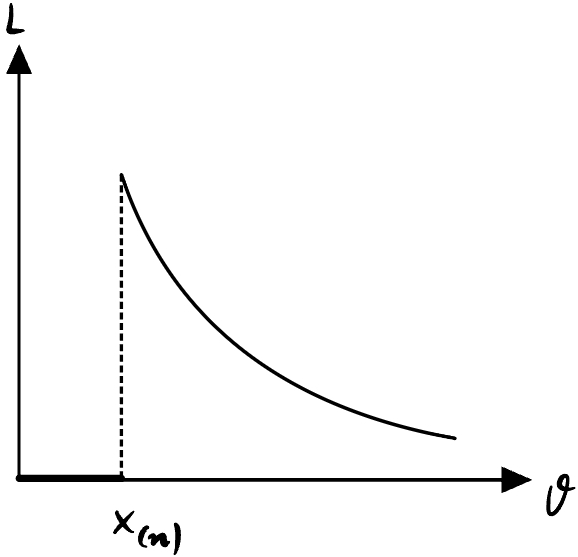
\includegraphics[width=0.17\textwidth]{Figura1.jpeg}
\end{wrapfigure}
\phantom{x}

In questo caso non serve fare calcoli, basta fare il disegno\\
Notiamo subito che il massimo della funzione L è in $X_{(n)}$\\
$ \implies \hat{\theta}_{MLE}=X_{(n)}$\\ \\

Confrontiamo questo caso tra i due metodi visti:
$\mu_1=\frac{\theta}{2}\implies \hat{\theta}_{MOM}=2\overline{X}_n$, mentre \ \ $\hat{\theta_{MLE}}=X_{(n)}$\\
In questo caso useremo $X_{(n)}$ perché è una statistica sufficiente, minimale e completa, quindi più comoda\\ \\


Esempio: $\camp\sim\Nc (\mu,\sigma^2)$
\[k=2 \ \ \ L(\mu,\sigma^2,\vv{x})=\frac{1}{(2\sqrt{2\pi\sigma^2})^2}  \, exp \OOO -\frac{1}{2\sigma^2}\Sum{i=1}{n} (x_i-\mu)^2 \CCC  \implies l(\mu,\sigma^2,\vv{x})=-\frac{n}{2} log (2\pi\sigma^2) - \frac{1}{2\sigma^2}\Sum{i=1}{n}(x_i-\mu)\]
Cerco i punti in cui la derivata di L cambia di segno e poi verifico se sono effettivamente massimi di L
\[ \begin{cases}
    \frac{\partial l}{\partial \mu}=\frac{1}{\sigma^2}\sum (X_i-\mu)\\
    \frac{\partial l}{\partial \sigma^2} = -\frac{n}{2}\frac{2\pi}{2\pi\sigma^2}+\frac{\sum (X_i-\mu)^2}{2(\sigma^2)^2}
\end{cases} \ \ \ \begin{cases}
    \frac{\partial l}{\partial \mu}\ge 0 \Leftrightarrow \sum X_i \ge n\mu \Leftrightarrow \mu \le \frac{\sum X_i}{n}\\
    \frac{\partial l}{\partial \sigma^2}\ge 0 \Leftrightarrow \frac{\sum (X_i-\mu)^2}{\sigma^2} \ge n \Leftrightarrow \sigma^2\le \frac{\sum (X_i-\mu)^2}{n}
\end{cases} \]   \[\text{ Nella 2° equazione ho il parametro $\mu$, lo devo sostituire con il suo stimatore: } \ \ \begin{cases}
    \hat{\mu}_{MLE}=\overline{X}_n\\
    \hat{\sigma^2}_{MLE}=\frac{\sum(X_i-\overline{X}_n)^2}{n}
\end{cases}\] \\



Proprietà di \textbf{invarianza} degli MLE dice che se $\hat{\theta}_{MLE}$ è lo stimatore MLE di $\theta \implies \ \forall \tau$ funzione di $\theta$,\\ lo stimatore MLE di $\tau(\theta)$ è $\tau(\hat{\theta}_{MLE})$, ovvero $\hat{\tau(\theta)}_{MLE}=\tau(\hat{\theta}_{MLE})$\\ \\

Esempio: $\camp\sim \Pc(\lambda)$ \ \ trovare l'MLE di $\prob{X_i=0}= e^{-\lambda}$\\
Userò la proprietà di invarianza, cerco $\hat{\lambda}_{MLE}$
\[L(\lambda,\vv{x})=\Prod{i=1}{n} \frac{e^{-\lambda}\lambda^{x_i}}{x!}\II_{\NN}(x_i)\]
\[\frac{\partial l}{\partial \lambda}=\Sum{i=1}{n} \frac{\partial}{\partial \lambda} \O log \O\frac{e^{-\lambda}\lambda^{X_i}}{X!}\C\C = \Sum{i=1}{n}\frac{\partial}{\partial \lambda} (-\lambda + X_i log\lambda) = \sum (-1 +\frac{X_i}{\lambda} = -n + \frac{\sum X_i}{\lambda})   \] 
\[ \frac{\partial l}{\partial \lambda}\ge 0 \Leftrightarrow \lambda\le \frac{\sum X_i}{n} \implies \hat{\lambda}_{MLE}=\overline{X}_n \]
\[ \implies \hat{(e^{-\lambda})}= e^{-\overline{X}_n} \text{per principio invarianza}\] \\

Esempio: Abbiamo appena calcolato lo stimatore $\hat{\sigma^2}_{MLE}$ per un campione gaussiano, allora vale:
\[\hat{\sigma}_{MLE}=\sqrt{\hat{\sigma^2}_{MLE}}=\sqrt{\frac{\Sum{i=1}{n}(X_i-\overline{X}_n)^2}{n}}\]

Esempio: Sapppiamo che $\hat{p}_{MLE}=\overline{X}_n$, allora
\[\sigma^2=\tau(p)=p(1-p)\implies \hat{\sigma^2}_{MLE}=\overline{X}_n(1-\overline{X}_n)\] \\




Restrizione del Range:\\
Se restringo lo spazio dei parametri da $\theta\in\Theta$ a $\theta \in \Theta_0 \subset \Theta$, \ allora \ \ $\hat{\theta^0_M}_{LE} = \underset{\theta\in\Theta_0}{ArgSup} L(\theta,\vv{x})$\\



\Lezione{03/03/2022}

\subsection{Analisi degli stimatori}

\begin{defi}
    Il MSE (mean squared error) è l'errore quadratico medio di uno stimatore $T$ per un parametro incognito $\theta$ ed è definito nel seguente modo: \ \ $MSE_{\theta}(T)=\EE_{\theta}[(T-\theta)^2]$
\end{defi}

\[MSE_{\theta}(T)=\EE_{\theta}[(T-\EE_{\theta}[T]+\EE_{\theta}[T]-\theta)^2]=\EE_{\theta}[(T-\EE_{\theta}[T])^2+(\EE_{\theta}[T]-\theta)^2+2(T-\EE_{\theta}[T])(\EE_{\theta}[T]-\theta)] = \]\[ =\EE_{\theta}[(T-\EE_{\theta}[T])^2] + (\EE_{\theta}[T]-\theta)^2 + 0\ \ \implies MSE_{\theta}(T)=Var_\theta[T]+(\EE_{\theta}[T]-\theta)^2\]\\
%
Definiamo la distorsione = bias := $\EE_{\theta}[T]-\theta $ \\
Se $\EE_{\theta}[T]-\theta =0$, allora T è detto non distorto per $\theta$ o unbiased\\

Oss. Tendenzialmente esiste un trade-off tra varianza e distorsione, per cui è difficile tenerli bassi entrambi\\

Dato $\camp $ \ la media campionaria $ \overline{X}_n$ è sempre uno stimatore non distorto della $\E{X_i}$\\
Infatti
$\E{\overline{X}_n}=\E{\frac{1}{n}\sum X_i}=\frac{1}{n}n\E{X}=\E{X}$\\

Dato $\camp\sim\Nc(\mu,\sigma^2)$ confrontiamo due stimatori della varianza\\
$S^2=\frac{1}{n-1}\Sum{i=1}{n}(X_i-\overline{X}_n)^2 \hspace{30pt} \hat{\sigma}^2_{MLE} = \frac{1}{n}\Sum{i=1}{n}(X_i-\overline{X}_n)^2=S_0^2$ \\
Oss. Possiamo sfruttare il fatto che $\frac{(n-1)S^2}{\sigma^2}\sim\Chi^2(n-1)\sim\Gamma\O\frac{n-1}{2},\frac{1}{2}\C$

\[MSE(S^2)=\var{S^2}+(\E{S^2}-\sigma^2)^2 =\OOO\OOO \E{S^2}=\frac{\sigma^2}{n-1}\E{\Chi^2(n-1)}=\sigma^2  \CCC\CCC= \var{S^2}= \]\[= \frac{\sigma^4}{(n-1)^2}\var{\Chi^2(n-1)}=\frac{\sigma^4}{(n-1)^2}(n-1)2=\frac{2\sigma^4}{n-1}\]
\[S_0^2=\frac{n-1}{n}S^2 \implies \ \text{Bias}=\E{S_0^2}-\sigma^2=\frac{n-1}{n}\sigma^2-\sigma^2=-\frac{\sigma^2}{n} \ \ \ \O S_0^2 \text{ sottostima }\sigma^2\C\]
\[ \implies \var{S_0^2}=\frac{(n-1)^2}{n^2}\var{S^2}=\frac{2\sigma^4(n-1)}{n^2}\]

\[MSE(S_0^2)=\frac{2\sigma^4(n-1)}{n^2}+\frac{\sigma^4}{n^2} = \frac{(2n+1)\sigma^4}{n^2}\]

\[\text{Confrontiamo i due MSE: } \hspace{30pt} \frac{2\sigma^4}{n-1} \hspace{30pt} \frac{(2n+1)\sigma^4}{n^2} \]
\[\text{Equivale al confronto tra: } \ \ \ \ \forall\sigma^2 \ \ \ \ (2n-1)(n-1)= 2n^2 -3n +1  \ \ \ \ \text{ e } \ \ \ \ 2n^2\]
\[\text{E quindi: } \ \ \ \ 1-3n \ \ \ \text{ e } \ \ \ 0  \ \ \ \
\ \ 
\text{ Dove il primo è sempre miore del secondo}\]\\
%
Qunidi $\forall \sigma^2 \ \ \ MSE_{\sigma^2}[S_0^2]<MSE_{\sigma^2}[S^2]$ \ \ ovvero mi conviene prendere uno stimatore distorto\\
Questo perchè la varianza è sempre inversa all'errore, quindi conviene sovrastimare l'errore per essere cauti\\

Definiamo le seguenti relazioni tra stimatori e parametri:\\
Se $\E{T}<\theta$ sottostima\\
Se $\E{T}>\theta$ sovrastima\\



In generale tra due stimatori $T_1$ e $T_2$ di $\theta$, scelgo lo stimatore con MSE inferiore\\
$T_1$ è preferibile a $T_2$ se $MSE_{\theta}(T_1)<MSE_{\theta}(T_2) \ \ \forall \theta$\\

Attenzione che il confronto tra MSE è un confronto tra due funzioni di $\theta$, potrebbe succedere che la disuguaglianza tra MSE non sia vera $\ \forall\theta$ \\
Ovvero che l'ordinamento del confronto tra MSE non è totale, potrebbero esserci stimatori non confrontabili\\ \\






Esempio: $\camp$ con $\Lc(x,\theta)$ che hanno $\theta=\E{X_i}$ e $1=\var{X_i}$\\
$T_1=\overline{X}_n \ \ T_2=a\overline{X_n}$\\
\[MSE_{\theta}[T_1]=Var_{\theta}[T_1]=\var{\frac{1}{n}\sum X_i}=\frac{1}{n^2}\cdot n\cdot 1=\frac{1}{n}\]
\[MSE_{\theta} [T_2] = \frac{a^2}{n}+(a\theta-\theta)^2=\frac{a^2}{n}+(a-1)^2\theta^2\]

% fatta la Figura1c in testo, ma brutta

\fg[]{0.3}{Figura1b.jpeg}

I due stimatori sono non confrontabili, però sceglierò la media campionaria, perché l'errore rimane "sotto controllo", mentre l'altro errore è quadratico\\ \\



Esempio: $X_1\sim \Pc(\lambda) \ \ \ T(X_1)=(-1)^{X_1}$ 
\[\E{T}= \E{(-1)^{X_1}}=\Sum{k=0}{+\infty}\OO(-1)^k\frac{e^{-\lambda}\lambda^k}{k!}\CC = e^{\lambda} \OO\Sum{k=0}{+\infty}\frac{(-\lambda)^k}{k!}\CC=e^{-2\lambda}\]
T è uno stimatore non distorto di $e^{-2\lambda}$ \ \ \  \ \ $T=\begin{cases}
    1 \ \ \text{ se $X_1$ è pari}\\
    -1 \ \ \text{ se $X_1$ è dispari}
\end{cases}$ \\

Oss. Sto però stimando con -1 la funzione $e^{-2\lambda}$  che è sempre positivo e non potrà mai essere -1, inoltre posso ricavare che il MSE non è tanto basso\\
Oss. Questo controesempio mi dice che non è detto che uno stimatore unbiased sia buono.
Proviamo a restringere il campo degli stimatori che cerchiamo\\


\begin{defi}
    Per UMVUE si intente uniform minimum variance unbiased estimator, ovvero stimatore non distorto a varianza uniformemente minima (rispetto a $\theta$)\\
    $T^*$ è \textbf{UMVUE} per $\theta$ se \ $\begin{cases}
        \EE_{\theta}[T^*]=\theta\\
         \E{T}=\theta \implies \var{T^*}\le\var{T}\  \ \ \  \forall \theta \ \ \  \forall T \text{ stimatore non distorto di } \theta
    \end{cases}$
\end{defi}
\phantom{}\\

\begin{teo}[Disuguaglianza di Cramer-Rao]
Siano $\camp \ iid $ con $ X_i\sim f(x_i,\theta) $ e $ T(\camp)$ stimatore di $\theta$. Assumiamo che:\\
i)\ supporto di $X_i$ non dipende da $\theta$ \ \ \ \ ii)\ $\E{T^2}<+\infty$ \smallskip \\
iii) \ $\frac{d \EE_{\theta}[T]}{d\theta}=\frac{d}{d\theta}\displaystyle\int_{\R^n} T(\vv{x})f(\vv{x},\theta)\,d\vv{x}=\int_{\R}T(\vv{x})\frac{\partial}{\partial \theta}f(\vv{x},\theta)\,d\vv{x}$
\[ \text{Allora} \ \ \ \ \ \ 0<\EE_{\theta}\OO\O\frac{\partial}{\partial\theta}\,log \,f(\vv{X},\theta)\C^2\CC<+\infty \ \implies \var{T}\ge\frac{\OO\frac{d}{d\theta}\EE_{\theta}[T]\CC^2}{\EE_{\theta}\OO\O\frac{\partial}{\partial\theta}\,log\,f(\vv{X},\theta)\C^2\CC}\]
\end{teo}

%
Oss. Nella famiglia esponenziale le condizioni sono rispettate\\
Oss. Inoltre se siamo nei non distorti, allora  $\frac{d}{d\theta}\EE_{\theta}[T] =1$\\

Informazione di Fisher = $I_n(\theta)=\EE_{\theta}\OO\O\frac{\partial}{\partial\theta}\,log\,f(\vv{X},\theta)\C^2\CC$\\
Oss. Detta informazione perché se ho I bassa significa che il limite sopra cui deve stare la varianza degli stimatori è alta e viceversa e quindi mi dice in anticipo che tipo di stimatori potrò trovare \\ \\

Nella classe degli stimatori non distorti il limite di C.-R. è $\frac{1}{I_n(\theta)} \ \implies \var{T}\ge\frac{1}{I_n(\theta)}$\\

Se io trovo uno stimatore T non distorto la cui varianza raggiunge il limite di C.-R. allora T è UMVUE\\
Però l'UMVUE può non raggiungere necessariamente il limite di C.-R.\\ \\


\Lezione{07/03/2023}


Esempio: Trovaiamo l'informazione di Fisher per delle Poisson \ \ \ $\camp\sim\Pc(\lambda)$ \[I_n(\lambda)=\E{\O\frac{\partial}{\partial \lambda}\,log\,f(\vv{X},\lambda)\C^2}
\]
\[\frac{\partial}{\partial\lambda}\,log\,f(\vv{X},\lambda)=\frac{\partial}{\partial\lambda}\,log\OO\Prod{i=1}{n}\frac{e^{-\lambda}\lambda^{X_i}}{X!}\CC=\Sum{i=1}{n}\frac{\partial}{\partial\lambda}\,log\,(e^{-\lambda}\lambda^{X_i})=\Sum{i=1}{n}\frac{\partial}{\partial\lambda}(-\lambda+X_i\,log\,\lambda)=\Sum{i=1}{n}\O-1+\frac{X_i}{\lambda}\C=\frac{n}{\lambda}\O\overline{X}_n-\lambda\C\]
\[\implies I_n(\lambda)=\E{\O\frac{n}{\lambda}(\overline{X}_n-\lambda)\C^2}=\frac{n^2}{\lambda^2}\E{\O\overline{X}_n-\lambda\C^2} = \frac{n^2}{\lambda^2}\var{\overline{X}_n}=\frac{n^2}{\lambda^2}\cdot\frac{\lambda}{n}=\frac{n}{\lambda} \skipp\skipp\]


Oss. Spesso aiuta, nel calcolo di I, riportarsi a una varianza nota, come abbiamo fatto qui\\

Abbiamo quindi ottenuto che $\var{T}\ge\frac{\OO\frac{d}{dx}\E{T}\CC^2}{I_n(\lambda)}=\frac{\lambda}{n}$ dato che lo stimatore è non distorto\\

Osservo che $\overline{X}_n$ è non distorto e $\var{\overline{X}_n}=\frac{\lambda}{n}$ \ cioè raggiunge il limite di C.-R. \ $\implies \overline{X}_n$ è UMVUE per $\lambda$\\

\begin{Dim}[Cramer-Rao]
La dimostrazione di C.-R. è un'applicazione della disuguaglianza di Cauchy-Schwarz:
\[ |\cov{X}{Y}|^2 \le \var{X}\var{Y} \skipp\]
%
Per dimostrare C.-S. \ considero una va \ $aX+Y$
\[
0\le\var{aX+Y}=\underset{\text{Polinomio di ordine 2 in a}}{\underbrace{a^2\var{X}+2a\cov{X}{Y}+\var{Y}}}\]
Ho quindi ottenuto una parabola che so essere sempre positiva e quindi ha determinate non positivo 
\[\Delta=4\cov{X}{Y}^2 -4\var{X}\var{Y}\le 0\]
\[\implies \var{X}\ge\frac{|\cov{X}{Y}|^2}{\var{Y}} \]
\phantom{}

Si useranno come variabili \ $X=T \ \text{ e } \ Y=\frac{\partial}{\partial\theta}\,log\,f(\vv{X},\theta)$\\

Per l'ipotesi iii) del teorema vale: \ \  \ $ \frac{d}{d\theta}\EE_{\theta}[T] = \displaystyle\int_{\R^n}T(\vv{x})\frac{\partial}{\partial \theta}f(\vv{x},\theta)\,d\vv{x} $
\[
\frac{\partial}{\partial\theta}\EE_{\theta}[T]\overset{(3)}{=} \int_{\R^n}T(\vv{x})\cdot\frac{\partial}{\partial\theta}f(\vv{x},\theta)\,d\vv{x} = \int_{\R^n}T(\vv{x})\cdot\frac{\partial}{\partial\theta}\,log\,f(\vv{x},\theta)\cdot f(\vv{x},\theta)\, d\vv{x} = \E{T\cdot Y}\]
\phantom{}

\[\text{Posto \ } T(\vv{X})=1 \ \text{ allora \ } \ 0=\frac{d}{d\theta}\E{1}=\int_{\R^n}\frac{\partial}{\partial\theta}\,f(\vv{x},\theta)\,d\vv{x}=\int_{\R^n}\frac{\partial}{\partial\theta}\,log\,f(\vv{x},\theta)\cdot f(\vv{x},\theta)\,d\vv{x} \]
\[\implies \ \E{Y}=0 \ \implies \ \cov{X}{Y}=\E{X\cdot Y} \ \text{ e } \ \var{Y}=\E{Y^2}\]\\

Adesso per ricavare C.-R. dobbiamo applicare C.-S.\\
\[\var{T}\ge\frac{\cov{T}{Y}^2}{\var{Y}}=\frac{\O\frac{d}{d\theta}\EE_{\theta}[T]\C^2}{\E{Y^2}}=\frac{\OO\frac{d}{d\theta}\EE_{\theta}[T]\CC^2}{\EE_{\theta}\OO\O\frac{\partial}{\partial\theta}\,log\,f(\vv{x}\theta)\C^2\CC}\]
\end{Dim}




Dalla dimostrazione si deduce che nella disuguaglianza C.-R. si raggiunge l'uguale quando \\ $X=T(\vv{x})$ è trasformazione lineare di $Y=\frac{\partial}{\partial\theta}\,log\,f(\vv{x},\theta)$




\subsubsection*{Ricerca dell'UMVUE}

\begin{teo}[Rao-Blackwell]
Siano T uno stimatore non distorto per $\theta$ e W una statistica sufficiente \\
Poniamo $M=\EE_{\theta}[T|W]$, \ allora M è ancora uno stimatore non distorto per $\theta$ e \ $\text{Var}_{\theta}[M]\le \text{Var}_{\theta}[T]$
\end{teo}

\begin{Dim}
1) M è uno stimatore
\[
M=\EE_{\theta}[T(\vv{X})|W]=\int_{\R^n} T(\vv{x})f(\vv{x}|W)\,d\vv{x} \] \[ \text{W è suff} \implies f(\vv{x}|W) \text{ non dipende da } \theta \implies \text{M stimatore}
\]
2) M è non distorto
\[
\EE_{\theta}[M]=\EE_{\theta}[\EE_{\theta}[T|W]]=\EE_{\theta}[T]=\theta
\]
3) $\var{M}\le\var{T}$
\[
\var{T}=\var{\EE_{\theta}[T|W]} + \underset{\ge0 \text{ perché var}\ge0}{\underbrace{\EE_{\theta}[\var{T|W}]}} \ \implies \var{M}\le\var{T}
\]
\end{Dim}

Vogliamo far vedere che con W non sufficiente, non vale il teorema

Esempio: $X_1,X_2\sim\Nc(\mu,1)$ \ \ \ $T=\frac{X_1+X_2}{2} \ \ \ \ W=X_1$
\[\E{T|W}=
\E{\overline{X}_2|X_1}=\frac12\OO\E{X_1|X_1}+\E{X_2|X_1}\CC= \frac12\O X_1+\mu\C \ \  \text{ Non è uno stimatore}
\]\\
%
\begin{teo}[Unicità dell'UMVUE]
    Sia $T(\vv{X})$ UMVUE per $\theta$, allora T è unico
\end{teo}

\begin{Dim}
    Supponiamo che esista un altro $T'$ UMVUE per $\theta$\\
    Ne costruisco un terzo. Sia $T^*=\frac12(T+T')$\\
    $T^*$ è uno stimatore e ha $\E{T^*}=\frac12(\E{T}+\E{T'})=\theta \ \implies$ \ anche $T^*$ è non distorto\\
    \[
    \var{T^*}=\frac14 \OO\var{T}+\var{T'}+2\cov{T}{T'}\CC \ \overset{C.-S.}{\le} \ \frac14\OO\var{T}+\var{T'}+2\sqrt{\var{T}\cdot\var{T'}}\CC
    \]
    Però dato che $T$ e $T'$ sono UMVUE allora devono avere stessa varianza
    $\implies \var{T^*}\le \var{T}$ Ma dato che T è UMVUE e $T^*$ è non distorto, in C.-S. vale l'uguaglianza $ \implies \var{T^*}=\var{T}$\\
    L'unico modo per cui questo è possibile è se $T'=aT+b$\\
    \[\var{T}=\cov{T}{T'}=\cov{T}{aT+b}=a\var{T} \implies a=1\]
    \[\E{T}=\E{T'}=\E{aT+b}=\E{T}+b \ \implies b=0\]
    \[\implies T=T' \implies \text{Se T esiste è unico}\]
\end{Dim}

\begin{teo}[Lemma di Scheffè 2]
    Sia T stimatore non distorto per $\theta$ (e quindi per ogni funzione $\tau(\theta)$)\\
    Sia W stat suff, minimale e completa per $\theta$\\
    Allora $M=\EE_{\theta}[T|W]$ è (l'unico) UMVUE per $\theta$
\end{teo}



\Lezione{13/03/20}


\begin{Dim}
    M è uno stimatore, dato che W è sufficiente (visto in Cramer-Rau)
    \[
    \EE_{\theta}[M]=\EE_{\theta}[\EE_{\theta}[T|W]]= \EE_{\theta}[T]=\theta
    \]
    Supponiamo che M non sia UMVUE, ovvero che esista uno stimatore T' non distorto di $\theta$ tc \ $\var{T'}<\var{T}$\\
    Usiamo teorema Rao-Blackwell su $T'$\\
    $M'=\E{T'|W}$ è uno stimatore non distorto di $\theta$ con $\var{M'}\le\var{T'}<\var{M}$\\

    Osserviamo che $M$ e $M'$ sono funzioni di $W$ e quindi $(M-M')$ è anch'essa funzione di $W$
    \[
    \E{M-M'}=0 \implies M-M' \text{ è una funzione } g(W) \text{ con media nulla, ma $W$ completo }\]
    \[\implies \prob{g(W)=0}=1 \implies M=M' \text{ qc}
    \]
    Ma questo contraddice l'affermazione che M non fosse UMVUE, quindi lo è ed è unico\\
\end{Dim}



Esempio: $\camp\sim Bi(k,\theta)$ con $k$ fissato e $\theta$ incognito

Cerchiamo l'UMVUE per $\tau(\theta)=\prob{X_i=1}=k\theta(\-\theta)^{k-1}$

Sappiamo che $W=\sum X_j$ è stat suff min completa per un campione binomiale, dove $W\sim Bi(nk,\theta)$

Però $\E{W}=nk\theta \ne \tau(\theta)$, quindi mi devo trovare uno stimatore che condizionato a $W$ mi dia $\tau$\\

Quando $\tau (\theta)$ è una probabilità, posso prendere delle bernulli che abbiano p uguale a $\tau$

\[
Y_1,...,Y_n \text{ tc } \   Y_i=\begin{cases}
    1 \ \ \ \text{ se } X_i=1\\
    0 \ \ \ \text{ se } X_i\ne 1
\end{cases} \ \ \implies \ \ Y_i\sim \II_{X_i=1} \sim Be (\prob{x_i=1}) = Be\O k\theta(1-\theta)^{k-1}\C
\]

Quindi $\overline{Y}_n =\frac1n \Sum{i=1}{n} Y_i$ è stimatore non distorto di $\tau(\theta)$\\

Adesso devo fare l'attesa condizionata, che è la parte più "contosa":
\[
\text{UMVUE per } \tau(\theta) \text{ è } \E{\overline{Y}_n \Big| \Sum{j=1}{n}X_j}  = \frac{1}{n} \Sum{j=1}{n} \E{Y_i \Big| \sum X_j } \ \overset{\text{sono iid}}{ = } \ \E{Y_1 \Big| \sum X_j }
\]
\[
\text{Però \ } \E{Y_1 \Big| \sum X_j = t } = \prob{Y_1=1 \Big| \Sum{j=1}{n} X_j =t } = \frac{\prob{Y_1=1 \cap \sum X_j =t}}{\prob{\sum X_j=t}} = \frac{\prob{X_1=1 \cap \sum X_j =t}}{\prob{\sum X_j=t}}= 
\]
Adesso gli eventi al numeratore non sono indipendenti, quindi non posso spezzare l'intersezione, però posso renderli indipendenti:
\[
=\frac{\prob{X_1=1 \cap \Sum{j=2}{n} X_j =t -1 }}{\prob{\sum X_j=t}} = \frac{\prob{X_1=1 } \prob{ \Sum{j=2}{n} X_j =t -1 }}{\prob{\sum X_j=t}}=
\]

Dove \ \ $X_j \sim Bi(k,\theta)$ \ \ $ \Sum{j=2}{n} X_j \sim Bi((n-1)k,\theta)  \ \ \Sum{j=1}{n} X_j \sim Bi(nk,\theta) $
\[
=\frac{k\theta (1-\theta)^{k-1} \binom{(n-1)k}{t-1} \theta^{t-1}(1-\theta)^{(n-1)k -t +1} }{\binom{nk}{t} \theta^t (1-\theta)^{nk-t}} = \frac{\binom{(n-1)k}{t-1} k }{\binom{nk}{t}  } = \E{Y_1 \big| \sum X_j =t}
\]

Quindi l'UMVUE per \  $k\theta(1-\theta)^{k-1}$ \  è \  \ $\displaystyle \frac{\binom{(n-1)k}{ \sum X_j -1 } k }{\binom{nk}{\sum X_j}  } = \E{\overline{Y}_n \big| \sum X_j } $\\



\subsection{Informazione di Fisher}

\begin{defi}
    Informazione di Fisher = $I_n(\theta)=\EE_{\theta}\OO\O\frac{\partial}{\partial\theta}\,log\,f(\vv{X},\theta)\C^2\CC$
\end{defi}

\textbf{Lemma1:}\\
Sia $\camp$ iid, allora $I_n(\theta)=nI_1(\theta)=n \E{\O\frac{\partial}{\partial\theta} \,log \,f(X_1,\theta)\C^2}$\\

\begin{Dim}[Lemma1]
    \[
    I_n(\theta)=\EE_{\theta}\OO\O\frac{\partial}{\partial\theta}\,log\, \Prod{i=1}{n} f(X_i, \theta)\C^2\CC = \EE_{\theta}\OO\O \Sum{i=1}{n} \frac{\partial}{\partial\theta}\,log\,  f(X_i, \theta)\C^2\CC  \]
    Quando lavoriamo con l'informazione di Fisher le ipotesi per la disuguaglianza di Cramer-Rao le ho sempre, quindi posso scambiare integrale e derivata e avevamo visto che grazie a questo vale:
    \[\E{ \frac{\partial }{\partial \theta} \, log\, f(X_i,\theta) }=0 \ \ \text{ quindi posso scrivere la media del quadrato con la varianza}\]
    \[
    I_n(\theta)= \var{\Sum{i=1}{n} \frac{\partial}{\partial\theta}\,log\,  f(X_i\theta)} \ \overset{ind}{ = } \  \Sum{i=1}{n}\var{ \frac{\partial}{\partial\theta}\,log\,  f(X_i,\theta)} \ \overset{iid}{ = } \ n \var{\frac{\partial}{\partial\theta}\,log\,  f(X_i,\theta)} =
    \]
    \[ \text{Per quanto detto prima } \ \ = n \E{ \O \frac{\partial}{\partial\theta}\,log\,  f(X_i,\theta)\C^2 } = n I_1(\theta) \]
\end{Dim}


\textbf{Lemma2:}\\
Se in aggiunta alle condizioni di Cramer-Rao si ha che: \ \ $ \frac{\partial }{\partial \theta} \OO \int_{\R^n} \frac{\partial }{\partial \theta} \, f(\vv{x}, \theta) \, d\vv{x}  \CC = \int_{\R^n} \frac{\partial^2}{\partial\theta^2}\, f(\vv{x},\theta)\, dx$\\
Allora $I_n(\theta) = - \EE_{\theta} \OO \frac{\partial^2}{\partial\theta^2}\, log \, f(\vv{x},\theta) \CC$\\




\begin{Dim}[Lemma2]
    \phantom{}\vspace*{-15pt}
    \[\E{\frac{\partial^2}{\partial\theta^2}\, log\, f(\vv{x},\theta)} = \int_{\R^n} \frac{\partial^2}{\partial\theta^2}\O log\, f(\vv{x},\theta)\C \cdot f(\vv{x},\theta)\, d\vv{x} = \int_{\R^n} \frac{\partial }{\partial \theta} \O \frac{ \frac{\partial }{\partial \theta} \, f(\vv{x},\theta)  }{f(\vv{x},\theta)}\C\, f(\vv{x},\theta) \, d\vv{x}=\] 
    \[= \int_{\R^n} \frac{\partial^2 }{\partial \theta^2} f(\vv{x},\theta)\cdot \frac{1}{f(\vv{x},\theta)} f(\vv{x},\theta)\, d\vv{x} + \int_{\R^n} - \frac{1}{f^2(\vv{x},\theta)}\cdot \O \frac{\partial }{\partial \theta} f(\vv{x},\theta)  \C^2 f(\vv{x},\theta) \, dx
    \]
    
    \[
    \text{ Per l'ipotesi del lemma } \ \ 
     \int_{\R^n} \frac{\partial^2}{\partial\theta^2}\, f(\vv{x},\theta)\, dx = \frac{\partial }{\partial \theta} \OO \int_{\R^n} \frac{\partial }{\partial \theta} \, f(\vv{x}, \theta) \, d\vv{x}  \CC = \]\[\frac{\partial }{\partial \theta} \OO \int_{\R^n} \frac{\partial }{\partial \theta} \, f(\vv{x}, \theta) \cdot \frac{1}{f(\vv{x}, \theta)} \cdot f(\vv{x}, \theta) \, d\vv{x}  \CC = \frac{\partial }{\partial \theta} \OO \E{ \frac{\partial }{\partial \theta}\, log \, f(\vv{x}, \theta)  } \CC =0
    \]
    \phantom{}
    
    In conclusione, abbiamo ottenuto che:
    \[
    \E{\frac{\partial^2}{\partial\theta^2}\, log\, f(\vv{x},\theta)} = - \int_{\R^n} \frac{1}{f^2(\vv{x},\theta)}\cdot \O \frac{\partial }{\partial \theta} f(\vv{x},\theta)  \C^2 f(\vv{x},\theta) \, dx =\]\[ = - \int_{\R^n} \O \frac{\partial }{\partial \theta} \, log\, f(\vv{x},\theta) \C^2 f(\vv{x},\theta) \, d\vv{x} = - I_n(\theta)
    \]
\end{Dim}


Oss. Quindi se ho delle $log \,L$ (log verosimiglianze) "piatte", cioè hanno una concavità bassa, avrò il limite di CR molto alto (stimatori con varianza alta) che non ci piace\\
Invece in situazioni in cui la $log\, L$ è poco piatta, vuol dire che ha derivata seconda negativa grande (concavità grande) e quindi il limite di CR è basso \\

Esempio: Campione gaussiano ha la $log L = -\Sum{i=1}{n} (x_i-\mu)^2$ che ha concavità alta e quindi ci piace\\


\begin{teo}
    $\camp$ iid con legge $f(X_i,\theta)$ appartenente EF, cioè \ \ $f(x,\theta) = h(x) x(\theta) \, exp \{w_1(\theta) t_1(x)\}$ tale che \ \ $\exists \frac{d}{d\theta} w_1(\theta)\ne 0 $ e continua \ $\forall \theta$ \ \ e \ $\Sum{j=1}{n} t_1(X_j)$ è sufficiente per $\theta$\\
    Allora le condizioni di CR sono soddisfatte e posto $T(\vv{X})=\frac{\Sum{j=1}{n} t_1(X_j)}{n}$, vale \[\var{T(\vv{X})} = \frac{ \O \frac{d}{d\theta} \EE_{\theta}\OO t_1(X)\CC \C^2 }{\E{\O \frac{\partial }{\partial \theta} \, log\, f(\vv{X},\theta)  \C^2 }} \]
    Quindi $T(\vv{X})$ è UMVUE per $\EE_{\theta} [t_1 (X_j)]$
\end{teo}

\phantom{}




\Lezione{14/03/20}


\begin{Dim}[*]
    Facciamo un'osservazione preliminare
    \[
    0=\frac{d}{d\theta} \int_{\R} f(x,\theta)\,dx = \frac{d}{d\theta} \int_{\R} h(x)c(\theta)\, exp\{w_1(\theta) t_1(x) \} \, dx = \]
    Posso portare dentro all'integrale la derivata perchè valgono le ipotesi di CR
    \[
    = \int_{\R} h(x) c'(\theta) exp\{w_1(\theta) t_1(x) \} \, dx + \int_{\R} h(x)c(\theta)exp\{w_1(\theta) t_1(x) \} \, w_1'(\theta) t_1(x)  \, dx = \]
    \[=\frac{c'(\theta)}{c(\theta)} \int_{\R} h(x) c(\theta) exp\{w_1(\theta) t_1(x) \} \, dx + w_1'(\theta) \int_{\R} h(x)c(\theta) exp\{w_1(\theta) t_1(x) \}\, t_1(x) \, dx=
    \]

    \[
    \text{Poichè } \ \ \int_{\R} h(x) c(\theta) exp\{w_1(\theta) t_1(x) \} \, dx = \int_{\R} f(x, \theta)\, dx = 1 \ \ \ \text{ e } \ \ \ \frac{c'(\theta)}{c(\theta)} = \frac{d}{d\theta} \, log \, c(\theta)
    \]
    \[
    \implies 0 = \frac{d}{d\theta} \, log \, c(\theta) + w'_1(\theta) \E{t_1(x)}
    \ \  \implies \ \ \EE_{\theta}[t_1(x)] = -\frac{1}{w_1'(\theta)}\cdot \frac{d}{d\theta} \, log\, c(\theta)
    \]
    Ho così scritto la media in funzione di $\theta$ invece che in funzione di x\\

    \[
    I_1(\theta)= \EE_{\theta}\OO \O \frac{\partial}{\partial\theta} \, log \, f(x,\theta) \C^2 \CC = \EE_{\theta} \OO \O \frac{\partial }{\partial \theta} \OO log\,h(x) + log \,c(\theta) + w_1(\theta)t_1(x) \CC  \C^2 \CC =\]
    \[ \EE_{\theta}\OO \O \frac{\partial }{\partial \theta}log\,c(\theta) + w_1'(\theta) t_1(x) \C^2 \CC = \O w_1'(\theta)\C^2 \EE_{\theta}\OO \O \frac{1}{w'_1(\theta)}\,\frac{\partial }{\partial \theta}log\,c(\theta) + t_1(x) \C^2 \CC = \]
    \[
    =  \O w_1'(\theta)\C^2 \EE_{\theta}\OO \O t_1(x) - \E{t_1(x)} \C^2 \CC = \O w_1'(\theta)\C^2 \OO \E{ \O t_1(x) \C^2 } - \E{t_1(x)}^2  \CC 
    \]
    \[
    \implies I_1(\theta)= \O w_1'(\theta)\C^2 \var{t_1(x)} \ \implies \ I_n(\theta) = n \O w_1'(\theta)\C^2 \var{t_1(x)}
    \]
    \phantom{}
    \[
    \frac{d}{d\theta} \E{t_1(x)} = \frac{d}{d\theta} \int_{\R} t_1(x)h(x)c(\theta) \, exp\{w_1(\theta) t_1(x) \}\, dx = ...\]
    \[
    \text{Con passaggi analoghi all'osservazione } \ = \frac{c'(\theta)}{c(\theta)} \int_{\R} t_1(x) f(x,\theta) \, dx + \int_{\R} \O t_1(x)\C^2 f(x,\theta) \cdot w_1'(\theta)\, dx =
    \]
    \[
    =\frac{d}{d\theta}\, log\,c(\theta) \EE \OO t_1(x) \CC + w_1'(\theta) \E{\O t_1(x)\C^2} = w_1'(\theta) \OO \E{\O t_1(x)^2\C} - \E{t_1(x)}^2 \CC = w_1'(\theta) \var{t_1(x)}
    \]
    \phantom{}
    
    A questo punto abbiamo numeratore e denominatore del limite CR e mettendo insieme, otteniamo:
    \[
    \text{Limite CR } = \frac{\O w'_1(\theta)\C^2 \var{t_1(x)}^2}{n\O w_1'(\theta)\C^2 \var{t_1(x)}} = \frac{\var{t_1(x)}}{n} = \frac{1}{n^2} \cdot n\var{t_1(x)} = \var{\frac{1}{n} \sum_j t_1(X_j) }
    \]
    Quindi abbiamo dimostrato che $T(X)=\frac{1}{n} \sum t_1(X_j)$ è UMVUE della sua media, ovvero $\E{t_1(X)}$\\
\end{Dim}


Esempio: $\camp \sim \Pc (\lambda) \ \ \ \ f(x,\lambda) = \frac{e^{-\lambda} \lambda^{-x}}{x!} \II_{\NN}(x) = \frac{\II_{\NN}(x)}{x!}\cdot e^{-\lambda} \, exp \{x\cdot log(\lambda)\}$\\
Qunidi $w_1'(x)=\frac{1}{\lambda} \ $ e sapendo che $ \ \frac{1}{n} \Sum{j=1}{n} t_1(X_j)$ è UMVUE per \ \  $-\frac{1}{w'_1(\lambda)}\cdot \frac{d}{d\lambda}\, log\, c(\lambda)$\\

Questo equivale a dire che per il campione gaussiano $\overline{X}_n$ è UMVUE per  $-\frac{1}{\frac{1}{\lambda}} \cdot \frac{d}{d\lambda} \, log \O e^{-\lambda}\C = \lambda$\\ \\


L'informazione di Fisher calcolata usando la legge del campione, coincide con quella calcolata usando la legge di una T statistica sufficiente\\


Questo perché avevamo visto che $f(\vv{x},\theta) = h(\vv{x}) g(T(\vv{x}),\theta)$
\[
\implies log\, f(\vv{x},\theta) = log\, h(\vv{x}) + log\, g(T(\vv{x}),\theta) \implies \frac{\partial }{\partial \theta} \,  lof \, f(\vv{x},\theta)= \frac{\partial }{\partial \theta} \, log\, g(T(\vv{x}),\theta)  
\]
E quindi nell'informazione di Fisher le due cose sono uguali\\




\subsection{Pillole sull'approccio bayesiano}

Noi avevamo visto $\theta$ come un parametro incognito, per l'approccio Bayesiano $\theta$ è vista come una variabile aleatoria, perché il suo valore non è fissato a priori\\

La legge di $\theta$ si chiamna Prior e viene indicata con $\Pi(\theta)$

Quindi quando scrivo la legge di $\vv{X}$ la scriverò $f(\vv{X}|\theta)$ perché è condizionata a una VA\\

Quando faccio inferenza, calcolo la legge di  $(\theta | \vv{x})$ e quindi la legge, detta a posterior $\Pi(\theta| \vv{x})$\\
Per il teorema di Bayes, ho: \ \ $\Pi(\theta | \vv{X}) = \frac{f(\vv{x}|\theta)\cdot \Pi(\theta)}{m(\vv{x})}= \frac{f(\vv{x}|\theta)\cdot \Pi (\theta)}{\int_{\Theta} f(\vv{x}|\theta) \Pi(\theta) \, d\theta} $\\ \\


Esempio: Modello beta-binomiale
\[
X_i|\theta \sim Be(\theta) \hspace{30pt} \Pi(\theta) \sim Beta(\alpha,\beta)
\]
\[
\Lc(\textstyle\sum X_i | \theta) \sim Bi (n,\theta) \hspace{30pt} \Pi(\theta | \sum X_i) \sim Beta (\alpha +  \sum X_i \, , \, n - \sum X_i + \beta)
\]
Per fare inferenza serve calcolare \ $\E{\Pi(\theta | \sum X_i)}$\\
Quindi scrivo la prior (a intuito) e poi fa l'esperimento e trova la condizionata $(\theta | \sum X_i)$  e trova la stima del parametro come la media della postirior:
\[
\Pi(\theta)\sim Beta (\alpha,\beta) \ \ \ \ \ \hat{\theta}_{\text{Bayes}}=\frac{\alpha + \sum X_i}{n+\alpha + \beta} = \frac{n}{\alpha + \beta +n}\O\frac{\sum X_i}{n}\C + \frac{\alpha+\beta}{\alpha +\beta +n} \O\frac{\alpha}{\alpha+\beta}\C
\]
Ma riscritta così possiamo vedere che la stima è una media convessa (ponderata) della media che avevo a priori e della media campionaria e vediamo che al crescere di n l'informazione della prior perde di valore e torniamo alla media campionaria\\


Oss. L'idea di approcciare $\theta$ come VA è molto elegante, però i modelli per cui si riescono ad affrontare questi conti sono pochi, per gli altri bisogna procedere con simulazioni. Inoltre rimane il grosso problema della scelta della prior







\newpage

\section{Test d'ipotesi}


Per test d'ipotesi si intende la verifica delle ipotesi statistiche


\begin{defi}
L'\textbf{ipotesi statistica} è un'affermazione su parametri incogniti $\vv{\theta}$ della legge di $\vv{X}$
\end{defi}

\begin{defi}
    In un problema di test d'ipotesi si introducono due ipotesi complementari:
    L'ipotesi nulla $H_0$ e  l'ipotesi alternativa $H_1$
\end{defi}

Oss. L'ipotesi statistica è la formulazione delle ipotesi nulla e alternativa, mentre il test d'ipotesi è un processo decisionale che ci porta a scegliere tra $H_0$ e $H_1$\\

Queste due ipotesi sono dette complementari perché se $H_0$ è tc $\vv{\theta}\in \Theta_0$,\\
Allora definiremo $H_1$ tc $\vv{\theta}\in \Theta_0^C$, ovvero sta nel complementare\\

\begin{defi}
    Un \textbf{test d'ipotesi} è una regola che specifica:\\
    a) Per quali valori di $\vv{x}$ accetto $H_0$\\
    b) Per quali valori di $\vv{x}$ rifiuto $H_0$ (accetto $H_1$)
\end{defi}
\phantom{}

Dovrò definire la regione critica \ \ $RC= \{ \vv{x}\in\R^n$ tc decido di rifiutare $H_0 \}$\\
$RC$ viene specificata sulla base dei valori assunti da una statistica test $W(\vv{x})$ \\

Oss. Nella definizione della regione critica, che è ciò che ci porta alla decisione, deve esserci solo il campione e la statistica, non può esserci il parametro incognito\\ \\


Esempio: Abbiamo delle bottigliette con scritto $500ml$, però vogliamo vedere se la media è più bassa.\\
Faremo dei tentativi per valutare se lo è veramente: \ \ $\camp \sim \Nc (\mu,\sigma^2)$

$H_0: \mu \ge 500ml \ \ \ \ \ \ H_1 : \mu<500ml$

Quindi definisco la regione critica come \ \  $RC:\{\overline{X}_n < 500-k\}$\\

Oss. Attenzione che non avremmo potuto definire $RC$ con $\mu$ al posto di $\overline{X}_n$

Oss. Tendenzialemnte $H_0$  è l'ipotesi "vera fino a prova contraria"\\ \\

\Lezione{20/03/20}


Vediamo dei metodi per costruire dei test d'ipotesi e dei metodi per valutarli e confrontarli


\subsection{Test del rapporto di verosimiglianza}

Detto anche LRT, cioè Likelihood ratio test\\


Date delle ipotesi $H_0: \theta\in \Theta_0 \ \ \ \ \ \ H_1 : \theta\in\Theta_0^C$, definiamo il LRT\\
\begin{defi}
    La statistica test per il LRT è \ \ $\lambda(\vv{x})= \frac{\displaystyle\sup_{\theta\in\Theta_0} L(\theta,\vv{x})}{\displaystyle\sup_{\theta\in\Theta}L(\theta,\vv{x})} = \frac{L(\hat{\theta}\,^0_{MLE})}{L(\hat{\theta}_{MLE})} $\smallskip\smallskip\\
    La regione critica è \ \ $RC= \{\lambda(\vv{x})\le c\}$ \ con \ $0\le c\le 1$
\end{defi}

Oss. $0\le \lambda(\vv{x})\le 1$ perché sappiamo che sia numeratore che denominatore sono positivi e il sup in un insieme più grande è sicuramente maggiore uguale\\

Oss. Ha senso porre la regione critica con $\le$ perché se $\lambda$ è piccolo, vuol dire che il sup in $\Theta_0$ è molto più piccolo del sup in $\Theta$, ma quindi è molto probabile che il parametro appartenga a $\Theta^C_0$\\ \\



Esempio: $\camp \sim \Nc (\theta,1) \ \ \ \begin{cases}
H_0 :  \ \theta =\theta_0\\
H_1 :  \ \theta\ne \theta_0
\end{cases}$\\
Oss. Al numeratore di $\lambda$ scriviamo direttamente $\theta_0$ perché è il sup in un punto
\[
\lambda(\vv{x}) = \frac{L(\theta_0, \vv{x})}{\sup_{\theta\in\Theta} L(\theta, \vv{x})} = \frac{L(\theta_0,\vv{x})}{L(\hat{\theta}_{MLE}, \vv{x})} = \frac{L(\theta_0,\vv{x})}{L(\overline{x}_n, \vv{x})}
\]
\[
\lambda(\vv{x}) = \frac{\O\frac{1}{2\pi}\C^{\tfrac{n}{2}} \, exp\OOO -\frac12 \Sum{i=1}{n} \O x_i -\theta_0  \C^2  \CCC }{\O\frac{1}{2\pi}\C^{\tfrac{n}{2}} \, exp\OOO -\frac12 \Sum{i=1}{n} \O x_i -\overline{x}_n  \C^2  \CCC} = exp \OOO \frac12 \OO -\Sum{i=1}{n} \O x_i -\theta_0  \C^2   + \Sum{i=1}{n} \O x_i -\overline{x}_n  \C^2 \CC \CCC
\]

Oss. $\Sum{i=1}{n} \O x_i -\theta_0  \C^2 = \Sum{i=1}{n} \O x_i -\overline{x}_n  + \overline{x}_n -\theta_0 \C^2 = \Sum{i=1}{n} \O x_i -\overline{x}_n  \C^2 + \Sum{i=1}{n} \O \overline{x}_n -\theta_0  \C^2 + 0$ 
\[
\implies \lambda(\vv{x})= exp\OOO -\frac{n}{2} \O \overline{x}_n -\theta_0 \C^2 \CCC
\]

\[
RC= \OOO exp\OOO -\frac{n}{2} (\overline{X}_n -\theta_0)^2 \CCC \le c \CCC = \OOO \O \overline{X}_n -\theta_0\C^2 \ge - \frac{2\, log\, c}{n} \CCC = \OOO \vv{x} \ : \ |\overline{X}_n -\theta_0| \ge \sqrt{-\frac{2\, log\, c}{n}} \CCC
\]
\phantom{}\smallskip
Oss. Questa regione critica ha senso perché equivale a valutare la distanza tra $\theta_0$ e $\overline{X}_n$ e se è maggiore di un certo valore allora rifiuto e questo ha senso perchè supponendo che $\theta_0$ sia vera, allora la media campionaria è disposta come una gaussiana centrata in $\theta_0$\\ \\


Esempio: $\camp\sim \theta + \Ec (1)$ \ \ \ $f(x,\theta) = exp\{-(x-\theta)\} \II_{[0,+\infty]}(x)$
\[
L(\theta,\vv{x}) = \Prod{i=1}{n} exp\{-(x_i-\theta)\} \II_{[0,\infty]}(x_i) = exp\OOO -\sum x_i +n\theta \CCC \II_{(-\infty,X_{(1)}]}(\theta)
\]
Guardando la funzione, concludo che $\hat{\theta}_{MLE}=X_{(1)}$ +++grafico \\


Test: $\begin{cases}
    H_0 : \ \theta\le \theta_0\\
    H_1 : \ \theta>\theta_0
\end{cases}$
\[
\lambda(x)=\frac{\sup_{\theta\le\theta_0 } L(\theta,\vv{x})}{\sup_{\theta\in\R}L(\theta,\vv{x})} = \frac{\sup_{\theta\le\theta_0 } L(\theta,\vv{x})}{L(X_{(1)},\vv{x})}
\]

+++grafici\\

Dato che la curva di L è crescente\\
Se $X_{(1)}\le \theta_0 \implies \sup_{\theta\le\theta_0} L(\theta,\vv{x})= L (X_{(1)},\vv{x})$\\
Se invece $X_{(1)}>\theta_0 \implies \sup_{\theta\le\theta_0} L(\theta,\vv{x}) = L(\theta_0, \vv{x})$\\
\[
\lambda(\vv{x}) = \begin{cases}
    \ \ 1 \ \ \ \ X_{(1)}\le \theta_0\\
    \frac{L(\theta_0,\vv{x})}{L(X_{(1)},\vv{x})} \ \ \ X_{(1)}>\theta_0
\end{cases} \ \ = \begin{cases}
    \ \ 1 \ \ \ \ X_{(1)}\le \theta_0\\
    exp\{-n(X_{(1)}-\theta_0) \} \ \ \ X_{(1)}>\theta_0
\end{cases}
\]

\[
RC= \{ e^{-n(X_{(1)}-\theta_0)} \le c \} = \{ X_{(1)}\ge \theta_0 - \frac{log\, c}{n} \}
\]

\phantom{}

\begin{teo}
Siano $T(\vv{X})$ stat suff per $\theta$ e $\lambda^*(t), \lambda(\vv{x})$ le statistiche LRT basate su $T$ e su $\vv{X}$
\[\text{Allora } \ \ \lambda^*(T(\vv{x}))=\lambda(\vv{x}) \ \ \forall \vv{x}\]
\end{teo}

\begin{Dim}
\[
\lambda(\vv{x}) = \frac{\sup_{\theta\in\Theta_0} L(\theta,\vv{x})}{\sup_{\theta\in\Theta}L(\theta,\vv{x})} \ \overset{\text{fattorizzazione }}{ = } \frac{\sup_{\theta\in\Theta_0} g(T(\vv{x}), \theta)\,\cancel{h(\vv{x})}}{\sup_{\theta\in\Theta}g(T(\vv{x}), \theta)\,\cancel{h(\vv{x})}} = \]
\[=\frac{\sup_{\theta\in\Theta_0} L^*(T(\vv{x}),\theta)}{\sup_{\theta\in\Theta}L^*(T(\vv{x}),\theta)} = \lambda^*(T(\vv{x}))
\]
\end{Dim}

\phantom{}


Oss. Adesso che abbiamo capito la LRT facciamo considerazioni su un test in generale

\subsection{Considerazioni di un test}
Prendiamo un test con una $RC$ e con le ipotesi $\begin{cases}
    H_0 : \ \theta\in \Theta_0\\
    H_1 : \ \theta\in \Theta_0^C
\end{cases}$\\ 

\begin{center}
\begin{tabular}{|c|c|c|}
\hline
 & Accetto $H_0$ & Rifiuto $H_0$\\
\hline
 $H_0$ vero & OK & Errore di I tipo\\
\hline
$H_1$ vero & Errore di II tipo & OK \\
\hline
\end{tabular}
\end{center}

Commettere un errore di I tipo è peggio di commettere un errore di II tipo\\


$\PP_{\theta}(\vv{X}\in RC) = \ \begin{cases}
    \text{probabilità di commettere un errore di I tipo \ \ se } \theta\in \Theta_0\\
    1-\PP_{\theta}(\vv{X}\not\in RC) =  1- \text{probabilità di commettere un errore di II tipo \ \ se } \theta\in \Theta_0^C
\end{cases}$\\ \\


\begin{defi}
    La \textbf{funzione potenza} di un test con regione critica $RC$ è:
    \[
    \beta(\theta) : \Theta \to [0,1] \ \ \ \ \beta(\theta)=\PP_{\theta}(\vv{X}\in RC)
    \]
\end{defi}

\phantom{}

La funzione potenza "ideale", sarebbe $\beta(\theta)= \begin{cases}
    0 \ \ \text{ se } \theta\in \Theta_0\\
    1 \ \ \text{ se } \theta\in\Theta_0^C
\end{cases}$\\

Oss. É impossibile riuscire ad avere una funzione così, perché l'unico modo per avere errore I =0 sarebbe quello di accettare sempre $H_0$, ma questo comporterebbe errore II = 1\\ \\



Esempio: Dati la VA e i test seguenti \ \ $X\sim Bi(5,\theta) \ \ \ \begin{cases}
    H_0 : \ \theta\le \frac12\\
    H_1 : \ \theta>\frac{1}{2}
\end{cases}$\\
Voglio confrontare le funzioni potenza di:\\
Test1: \ \ $RC_1 =\{X=5\}$\\
Test2: \ \ $RC_2 = \{X\ge3\}$\\

$\beta_1(\theta)=\PP_{\theta}(X=5)=\theta^5$\\
$\beta_2(\theta)=\PP_{\theta}(X\ge3) = \binom{5}{3}\,\theta^3(1-\theta)^2 + 5\,\theta^4(1-\theta) +\theta^5$\\
+++grafico\\

Le due funzioni sono crescenti, quindi per entrambe vale che $\prob{\text{errore I tipo}} \le \PP_{\theta_0}(RC) = \beta(\theta_0)$\\

$\beta_1(\theta_0)=\O\frac12\C^5=0,03125$ \ \ \ \ che è un buon limite\\
$\beta_1(\theta)\ge0,8 \implies \theta\ge0,96$ quindi questo test va bene in $\Theta_0$, ma fuori non è molto forte\\

$\beta_2(\theta_0)= (10 + 5 +1 )\O\frac12\C^5 = \frac12$ \ \ che è troppo alta\\ \\

\Lezione{21/03/2023}\\

Esempio: $\camp \sim \Nc (\mu,\sigma^2)$ \ con  $\sigma^2$ noto\\
LRT per \ $\begin{cases}
    H_0 \ \ \mu\le \mu_0\\
    H_1 \ \ \mu>\mu_0
\end{cases}$ \ \ con $RC = \OOO \frac{\overline{X}_n -\mu_0}{\tfrac{\sigma}{\sqrt{n}}} >c \CCC$
\[
\beta(\mu) = \PP_{\mu}\O\frac{\overline{X}_n -\mu_0}{\tfrac{\sigma}{\sqrt{n}}}>c\C = \PP_{\mu} \O\underset{Z}{\underbrace{\frac{\overline{X}_n -\mu}{\tfrac{\sigma}{\sqrt{n}}}}} > c + \frac{\mu_0-\mu}{\tfrac{\sigma}{\sqrt{n}}}\C = 1 - \Phi \O c +\frac{\mu_0-\mu}{\tfrac{\sigma}{\sqrt{n}}}  \C
\]
Al crescere di $\mu$, \ \ $\frac{\mu_0-\mu}{\tfrac{\sigma}{\sqrt{n}}}$ decrcesce, \ \ $\Phi$ decresce \ \ e quindi $\beta$ è crescente in $\mu$
\[
\lim_{\mu\to-\infty} \beta(\mu) =0 \ \ \ \  \lim_{\mu\to +\infty} \beta(\mu) =1 \ \ \ \ \beta(\mu_0)= 1-\Phi(c)
\]
Inoltre per modificare la crescita di questa curva, l'unica cosa che possiamo fare è modificare n\\
Al crescere di $n$ la funzione cresce più velocemente\\ 


Vogliamo controllare (limitare) la massima probabilità di commettere un errore di I tipo

\[\sup_{\mu\le\mu_0} \beta(\mu) = \beta(\mu_0)\]
\[\beta(\mu_0)=0.10 \ \Longleftrightarrow \ 1-\Phi(c)=0.10  \ \Longleftrightarrow \ c= Z_{0.9}=1.28\skipp\]

Vogliamo che la funzione potenza sia $\ge 0.8$ per $\mu\ge\mu_0+\sigma$, ovvero che oltre a quel punto la probabilità di commettere un errore II tipo sia minore del $20\%\,$, per far ciò devo imporre:
\[
0.8 = \beta(\mu_0+\sigma) = 1-\Phi\O1.28-\frac{\sigma}{\tfrac{\sigma}{\sqrt{n}}}\C = 1 - \Phi(1.28-\sqrt{n}) \Longleftrightarrow \Phi(1.28-\sqrt{n})=0.2
\]
\[
\Longleftrightarrow 1.28 -\sqrt{n} = Z_{0.2} = -0.84 \Longleftrightarrow n= 4.49 \Longleftrightarrow  n\ge 5\]

++++GRAFICO\\ \\


\begin{defi}
    $\forall \, 0\le \alpha\le 1 $ un test con funzione potenza $\beta(\theta)$ è detto di \textbf{dimensione} $\alpha$ se il $\displaystyle \sup_{\theta\in\Theta_0} \beta(\theta)=\alpha$
\end{defi}

\begin{defi}
    $\forall \, 0\le \alpha\le 1 $ un test con funzione potenza $\beta(\theta)$ è detto di \textbf{livello} $\alpha$ se il $\displaystyle \sup_{\theta\in\Theta_0} \beta(\theta)\le\alpha$
\end{defi}

Oss. Queste definizioni si usano per controllare gli errori di I tipo\\ \\

Esempio: $\camp $ iid \ \ $f(X,\theta) = e^{-(x,\theta)} \II_{[\theta,+\infty)}$ \ \ con \ \ $\begin{cases}
    H_0 : \ \theta\le \theta_0\\
    H_1 : \ \theta>\theta_0
\end{cases}$

Avevamo trovato LRT  con  $RC = \OOO X_{(1)}\ge \theta_0 - \frac{log \, c}{n} \CCC$ \\

LRT serve per trovare una "forma" di regione critica, quello che poi dobbiamo fare è imporre il livello\\

Voglio un test LRT di livello $\alpha$, ovvero \ \ $\displaystyle \sup_{\theta\le \theta_0} \beta(\theta) = \sup_{\theta\le \theta_0} \PP_{\theta}(RC) \le \alpha$
\[
\beta(\theta)= \PP_{\theta} \O X_{(1)}\ge \theta_0 -\frac{log\, c}{n} \C
\]
Avevamo trovato che $X_i = \theta T_i$ \ con \ $T_i\sim \Ec (1)$
\[
\implies min X_i = min (\theta +T_i)= \theta + T_{(1)} \ \ \ \ T_{(1)}\sim \Ec(n)
\]
\[
\PP(X_{(1)}\ge k) = e^{-n(k-\theta)} \ \ \ \ \text{ questa funzione è crescente in } \theta
\]
\[
\beta(\theta)= exp\OOO-n\O\theta_0 -\frac{log\, c}{n} -\theta\C\CCC \ \ \ \ \alpha=\sup_{\theta\le\theta_0} \beta(\theta) = \beta(\theta_0) = exp\OOO-n\O\theta_0 -\frac{log\, c}{n} -\theta_0\C\CCC = c
 \]

\phantom{}\\

\begin{defi}
    Un test con funzione potenza $\beta(\theta)$ è detto \textbf{non distorto} se \ \ $\beta(\theta')\le\beta(\theta'') \ \ \ \forall \theta'\in \Theta_0^C \ \ \forall \theta''\in\Theta_0$
\end{defi}



\begin{defi}
    Sia $C$ una classe di test per verificare $H_0: \ \theta\in \Theta_0$ \ VS \ $H_1: \ \theta\in\Theta_0^C$\\
    Allora un test in $C$ con funzione potenza $\beta(\theta)$ è \textbf{UMP}, uniformly most powerful,\\ se $\beta(\theta)\ge\beta'(\theta) \ \ \forall \theta\in\Theta_0^C$ e $\forall\beta'(\theta)$ funzione potenza di test in $C$\\
    Tipicamente $C$ è la classe funzione dei test di livello $\alpha$
\end{defi}

Oss. L'idea è che sono sicuro di non avere problemi in $\Theta_0$ perché ho chiesto che la classe sia di livello $\alpha$, quindi la $\beta$ più forte è quella più forte in $\Theta_0^C$\\ \\


Oss. Il seguente lemma parte da una situazione più facile e generalizza in seguito

\begin{teo}[Lemma di Neymann-Pearson]
     Usando le "ipotesi semplici", ovvero $H_0 : \ \theta=\theta_0$ \ VS \ $H_1: \ \theta=\theta_1$\\
     Per $\beta$ ci serviranno solamente $f(\vv{x},\theta_i)$ per $i=0,1$ \\
     Sia $RC$ tale che:\\
     1) \ $\vv{x}\in RC$ se $f(\vv{x},\theta_1)>kf(\vv{x},\theta_0)$\ \ \ e \ \ \ $\vv{x}\in RC^C$ se $f(\vv{x},\theta_1)<k f(\vv{x},\theta_0)$ \ \ \ con $k\ge0$\\
     2) \ $\alpha = \PP_{\theta_0}(\vv{x}\in RC)$\\
     Allora:\\
     a) \ Qualunque test che soddisfa 1) e 2) è UMP di livello e dimensione $\alpha$\\
     b) \ Se esiste un test che soddisfa 1) e 2) con $k>0$\\
     \phantom{b) \ }Allora ogni test UMP di livello $\alpha$, ha anche dimensione $\alpha$ (soddisfa  la 2))\\
     \phantom{b) \ }E soddisfa la 1) tranne che su un insieme $A$ \ tc \ $\PP_{\theta_0}(\vv{x}\in A)= \PP_{\theta_1}(\vv{x}\in A)=0$
\end{teo}

Oss. Quindi poste le ipotesi semplici,  che mi fanno scegliere tra due valori del parametro\\
Questo lemma si basa su un'idea simile alle "classi di equivalenza dei test" e dice che un test con 1) e 2) è UMP e se invece prendo un test UMP, allora sarà "quasi" uguale al test con 1) e 2)\\ 

\begin{Dim}[Neymann-Pearson*]
    La 2) equivale a dire che il test è di dimensione $\alpha$\\
    Prendiamo $\Phi(\vv{x})$ una funzione test \ \ \ $\Phi(\vv{x})=\II_{RC}(\vv{x})$\\

    \textbf{a)}\\
    Siano $\Phi(\vv{x})$ la funzione test di un test che soddisfa  1) e 2)  \ \ con funzione potenza $\beta(\theta)$ \\
    E \ $\Phi'(\vv{x})$ la funzione test di un altro test di livello $\alpha$ \ \ con \ $\beta'(\theta)$
    \[
    (\Phi(\vv{x})-\Phi'(\vv{x}))\cdot (f(\vv{x},\theta_1)-k  f(\vv{x},\theta_0))\ge 0 \ \ \forall \vv{x}
    \]
    Se $\vv{x}\in RC$, definita da 1), allora questa diventa:
    \[
    (1-\Phi'(\vv{x}))\underset{\ge0}{\underbrace{(f(\vv{x},\theta_1)-kf(\vv{x},\theta_0))}}
    \]
    Se $\vv{x}\in RC^C$, per la 1)
    \[
    (0-\Phi'(\vv{x}))\underset{\le 0}{\underbrace{f(\vv{x},\theta_1-f(\vv{x},\theta_0))}}
    \]
    Avevamo ottenuto che:
    \[
    \int_{\R^n} (\Phi(\vv{x})-\Phi'(\vv{x}))(f(\vv{x},\theta_1)-k  f(\vv{x},\theta_0)) \, d\vv{x}\ge 0
    \]
    Poichè $\int_{\R^n}\II_{B}(\vv{x})\, d\vv{x} = \PP(\vv{x}\in B)$
    \[
    0\le \PP_{\theta_1}(RC) - \PP_{\theta_1}(RC') - k\PP_{\theta_0}(RC) + k\PP_{\theta_0}(RC') = \beta(\theta_1) - \beta'(\theta_1) - k\big(\beta(\theta_0)- \beta'(\theta_0)\big)
    \]
    So che $\Phi$ soddisfa la 2) \ $\implies \beta(\theta_0)=\alpha$\\
    E so che $\Phi'$ è di livello $\alpha$ \ $\implies \beta'(\theta_0)\le \alpha$
    \[
    \implies \beta(\theta_0)-\beta'(\theta_0)\ge 0 \ \implies \beta(\theta_1) - \beta'(\theta_1) \ge 0 \implies \ \Phi \text{ è UMP, oltre che essere di livello e dimensione } \alpha    \]

    \phantom{}

    \textbf{b)}\\
    Sia $\Phi'$ la funzione test di test UMP di livello $\alpha$, ma da a) so che $\Phi$ (che soddisfa 1) e 2)) è UMP di liv $\alpha$
    \[
    \implies \beta(\theta_1)=\beta'(\theta_1)
    \]
    So che \ $\beta'(\theta_0)\le \alpha$ \ \ e da a) so che $0\le -k(\beta(\theta_0)-\beta'(\theta_0)) \implies 0\ge(\alpha-\beta'(\theta_0))\implies \beta'(\theta_0)\ge\alpha$ \\
    $\implies \beta'(\theta_0) =\alpha$ \ \  
    quindi soddisfa 2)\\

    \[
    \beta(\theta_1) -\beta'(\theta_1) - k(\beta(\theta_0)- \beta'(\theta_0)) = \int_{\R^n} (\Phi(\vv{x})-\Phi(\vv{x}))(f(\vv{x},\theta_1)-kf(\vv{x},\theta_0))\,d\vv{x}
    \]

    $\implies \Phi = \Phi'$ \ tranne che su un insieme A con $\PP_{\theta_0}(\vv{x}\in A)=\PP_{\theta_1}(\vv{x}\in A)$
\end{Dim}
\phantom{}

\Lezione{27/03/23}

Oss.
$\begin{cases}
    H_0 : \ f_0(\vv{x})\\
    H_1 : \ f_1(\vv{x})
\end{cases}$ \ \ non devono essere della stessa famiglia parametrica\\

Esempio: 13.1\\

\textbf{Corollario:}\\
Dato \ $\begin{cases}
    H_0 \ : \ \theta=\theta_0\\
    H_1 \ : \ \theta=\theta_1
\end{cases}$ \ sia $T(\vv{X})$ una statistica sufficiente per $\theta$ e $g(t,\theta)$ la legge di $T(\vv{X})$\\
Allora il test UMP di livello $\alpha$ basato su T è quello con $RC=\{g(t,\theta_1)>kg(t,\theta_2)\}$\\

Oss. Vale perché $f(\vv{x},\theta)=g(t,\theta)h(\vv{x})$\\

Esempi: 13.2 \ 13.3 \ 13.4\\


\begin{defi}
    Data una famiglia di leggi $\{f(x,\theta), \ \theta\in \Theta\}$, la famiglia è detta a MLR, o likelihood ratio monotona (non decrescente)  se \ $\frac{f(x,\theta_1)}{f(x,\theta_2)}$ è monotona non decrescente in x \ $\forall\theta_1>\theta_2$
\end{defi}

\phantom{}

Esempi: 13.5 \ 13.6\\


\begin{teo}[Karlin-Rubin]
    Dato $\begin{cases}
        H_0 : \ \theta\le \theta_0\\
        H_1 : \ \theta> \theta_0
    \end{cases}$
    \ \  \ Se T è stat suff per $\theta$ tale che la legge di $T$, ovvero $g(t,\theta)$, ha MLR\\
    Allora $\ \forall t_0$ il test con $RC= \{ T>t_0 \}$ è UMP di livello $\alpha = \PP_{\theta_0}(T>t_0)$ 
\end{teo}

Oss. Ovvero quando ho l'ipotesi in questo modo e ho a disposizione una statistica suff con legge MLR\\



\begin{Dim}
    \[
    \beta(\theta) = \PP_{\theta} (T>t_0)
    \]
    Mostriamo che $T$ ha MLR $\implies$ la funzione potenza $\beta(\theta)$ è non decrescente in $\theta$\\
    Posto $\theta_1<\theta_2$ e data la $F(t,\theta)$ la funzione di ripartizione di $T$
    \[
    \frac{d}{d t}[F(t,\theta_1)- F(t,\theta_2)] = g(t,\theta_2)-g(t,\theta_1) = g(t,\theta_1) \OO \UB{\text{crescente in t}}{\frac{g(t,\theta_2)}{g(t,\theta_1)}} -1 \CC
    \]
    Questa derivata essendo crescente o è sempre positiva oppure passa da negativa a positiva\\
    Quindi $[F(t,\theta_1)- F(t,\theta_2)]$ è o sempre crescente, oppure prima decresce e poi cresce\\
    E quindi questa differenza raggiunge il massimo in $-\infty$ oppure in $+\infty$\\

    Ma essendo funzioni di ripartizione vanno entrambe da 0 a 1 e quindi
    \[
    \begin{cases}
        F(-\infty,\theta_2)-F(-\infty,\theta_1)=0\\
        F(+\infty,\theta_2)-F(+\infty,\theta_1)=0
    \end{cases}
    \]
    \[
    \implies \ \ \ \ F(t,\theta_2)-F(t,\theta_1)\le 0  \Longleftrightarrow F(t,\theta_2)\le F(t,\theta_2)
    \]
    \[
    \beta (\theta_1)= \PP_{\theta_1} = 1- F(t_0,\theta_1)\le 1- F(t_0,\theta_2)= \PP_{\theta_2}(t>t_0) = \beta(\theta)
    \]

    \phantom{}
    
    Oss. Definiamo X stocasticamente più grande di Y, $X \underset{st}{\ge} Y$, se $F_X(t)\le F_Y(t)$\\
    Esempi: 10.7 \ 10.8\\
    
    Quindi se T ha MLR allora $\beta(\theta)$ è crescente
    \[
    \implies \sup_{\theta\le\theta_0} \beta(\theta)=\beta(\theta_0) \implies \text{ il livello è } \alpha=\PP_{\theta_0}(RC) = \PP_{\theta_0}(T>t_0)
    \]
    \phantom{}

    Partendo dal caso
    $\begin{cases}
        H_0 : \ \theta=\theta_0\\
        H_1 : \ \theta = \theta' 
    \end{cases}$ \ \ \ con $\theta'>\theta_0$\  \ quindi ho un'ipotesi semplice inclusa nel caso generale
    \[
    \text{Allora } \  \tilde{K}= \inf_{\tau=\{t>t_0\}} \frac{g(t,\theta')}{g(\theta_0)}
    \]
    \[
    T>t_0 \Longleftrightarrow \frac{g(t,\theta')}{g(\theta_0)} >\tilde{K}
    \]
    \[
    T>t_0 \Longleftrightarrow \OOO g(t,\theta')>\tilde{k}g(t,\theta_0) \CCC \ \ \text{ è UMP per il corollario di N-P} 
    \]
\end{Dim}


Si può dimostrare il teorema nel caso opposto: \ $\begin{cases}
    H_0 : \ \theta\ge\theta_0\\
    H_1 : \ \theta < \theta_0 
\end{cases}$ \\ 
In cui si ha UMP con $RC : \{T<t_0\} \ \ \alpha=\PP_{\theta_0}(T<t_0)$\\ \\

\Lezione{28/03/23}

\begin{defi}
    Un test è detto \textbf{Test Unione Intersezione}, o test UI\\ Se \ $\Theta_0$ si può scrivere come un'intersezione di sottoinsiemi di $\Theta$ e se\\
    $H_0 : \ \theta\in \Theta_0 = \underset{\gamma\in\Gamma}{\bigcap} \Theta_{0\gamma}$ \ \ VS \ \ $H_1 : \ \theta\in\Theta_0^C= \underset{\gamma\in\Gamma}{\bigcup} \Theta_{0\gamma}^C$\\
    $\forall\,\gamma \ \ \ H_{0\gamma} : \  \theta_0\in\Theta_{0\gamma} \ \text{ VS } \ H_{1\gamma} : \ \theta\in \Theta_{0\gamma}^C$ \ \ con $RC_{\gamma}$\\
    $\implies RC$ del test UI è $RC=\underset{\gamma\in\Gamma}{\bigcup}  RC_{\gamma}$ 
\end{defi}

Oss. Complementare dell'intersezione è l'unione dei complementari\\
Oss. La $RC$ è unione perché devo accettare tutti gli $H_{0\gamma}$


Esempio: 14.1\\


\begin{defi}
    Un test è detto \textbf{intersezione unione}, o test IU, quando si può scrivere
    \[
    H_0 : \ \theta\in \Theta_0 = \underset{{\gamma\in\Gamma}}{\bigcup} \Theta_{0\gamma} \ \ \text{ VS } \ \ H_1 : \ \theta\in \Theta_0^C = \underset{{\gamma\in\Gamma}}{\bigcap} \Theta_{0\gamma}^C
    \]
    \[
    RC_{IU}= \underset{\gamma\in\Gamma}{\bigcap} RC_{\gamma}
    \]
\end{defi}


Esempio: 14.2\\ \\




\begin{teo}
Dato un test UI \ \ $\begin{cases}
    H_0 : \ \theta\in \underset{\gamma\in\gamma}{\bigcap} \Theta_{0\gamma}\\
    H_1 : \ \theta\in \underset{\gamma\in\gamma}{\bigcap} \Theta_{0\gamma}^C
\end{cases}$\\
Chiamiamo $\lambda_{\gamma}(\vv{x})$ la statistica del LRT per $H_{0\gamma}=\theta\in\Theta_{0\gamma}$\\
e $\lambda(\vv{x})$ la statistica del LRT per il test UI\\
Sia $T(\vv{x})=\displaystyle\inf_{\gamma} \lambda_{\gamma}(\vv{x})$ e siano
    \[
    RC_T = \{ \lambda_{\gamma}(\vv{x})=c \ \ \text{ per qualche } \gamma\} = \{T(\vv{x})\le c\}
    \]
    \[
    RC_{\lambda}=\{\lambda(\vv{x})\le c\}
    \]
    Allora:\\
    a) \ $T(\vv{x})\ge \lambda(\vv{x}) \ \ \forall \vv{x}$\\
    b) \ $\beta_T(\theta)\le \beta_{\lambda}(\theta) \ \ \forall\theta$\\
    c) \ Se il LRT ha livello $\alpha$, allora il test UI ha livello $\alpha$
\end{teo}

\begin{Dim}
    a)
    \[
    \Theta_0=\underset{\gamma\in\Gamma}{\bigcap} \Theta_{0\gamma} \ \implies \Theta_0 \subset \Theta_{0\gamma} \ \forall\gamma
    \]
    \[
    \lambda_{\gamma}(\vv{x})= \frac{\sup_{\Theta_{0\gamma}}L(\theta,\vv{x})}{\sup_{\Theta}L(\theta,\vv{x})} \ge  \frac{\sup_{\Theta_0}L(\theta,\vv{x})}{\sup_{\Theta}L(\theta,\vv{x})} = \lambda(\vv{x}) 
    \] 
    \[
    \implies T(\vv{x}) = \inf_{\gamma}\lambda_{\gamma}(\vv{x})\ge \lambda(\vv{x})
    \]

    b)
    \[
    \beta_T(\theta)=\PP_{\theta}(T(\vv{x})\le c) \le \PP_{\theta}(\lambda(\vv{x})\le c) = \beta_{\lambda}(\theta)
    \]

    c)
    \[
    \text{Livello test UI } = \sup_{\theta\in\Theta_0}\beta_T(\theta) \le \sup_{\theta\in\Theta_0} \beta_{\gamma}(\theta)\le\alpha
    \]
\end{Dim}

\begin{teo}
Dato un test IU con $\Theta_0 = \underset{\gamma\in\Gamma}{\Theta_{0\gamma}}$\\
Sia $\alpha_{\gamma}$ il livello del test su $\Theta_{0\gamma}$ con $RC_{\gamma}$ allora il test IU ha livello $\alpha= \displaystyle\sup_{\gamma} \alpha_{\gamma}$
\end{teo}

\begin{Dim}
    \[
    \theta\in\Theta_0 \implies \theta\in\Theta_{0\gamma} \text{ per qualche } \gamma
    \]
    \[
    \PP_{\theta}(\vv{x}\in RC) \le \PP_{\theta}(\vv{x}\in RC_{\gamma}) \le \alpha_{\gamma}\le \sup_{\gamma} \alpha_{\gamma}
    \]
\end{Dim}

\phantom{}


Vediamo questo teorema in un caso particolare del test IU, dove l'insieme dei $\Theta_{0\gamma}$ ha un numero di indici ben definito\\


\begin{teo}
    Dato un test IU con $H_0 : \ \theta\in \cup_{j=1}^k \Theta_{0j}$ e $RC_j$ la RC del test $H_0 : \theta\in \Theta_{0j}$\\
    Supponiamo che per qualche $i=1...k$ \ $\exists$ una successione di parametri $\theta_l \in \Theta_{0i}$ tale che\\
    \[
    1) \lim_{l\to+\infty} \PP_{\theta_l} (\vv{x}\in RC_i)=\alpha
    \]
    \[
    2) \lim_{l\to\infty} \PP_{\theta_l} (\vv{x}\in RC_j)= 1 \ \ \ j=1...k \ j\ne i
    \]
    Allora il test IU con $RC=\bigcap_{j=1}^n RC_j$ ha livello $\alpha$ 
\end{teo}

\begin{Dim}
    Dal teorema precedente \ $RC$ ha livello $\alpha$, vogliamo mostrare che ha proprio dimensione $\alpha$
    \[
    \theta_l \in \Theta_{0i} \in \Theta_0 = \underset{j}{\cup} \Theta_{0j}
    \]
    \[
    \implies \sup_{\theta\in\Theta_0} \PP_{\theta}(\vv{x}\in RC) \ge \lim_{l\to+\infty} \PP_{\theta_l} (\vv{x}\in RC) = \lim_{l\to +\infty} \PP_{\theta_l} (\vv{x}\in \underset{j}{\cap} RC_j) \ge\]
    Vale per la disuguaglianza di Bonferroni \ $\displaystyle\prob{\bigcap_{i=1}^n A_i}\ge \Sum{j=1}{n} \prob{A_i} - (n-1)$
    \[
    \ge \lim_{t\to+\infty} \Sum{j=1}{k} \PP_{\theta_l} (\vv{x}\in RC_j) - (k-1) = (k-1)\cdot 1 +\alpha -(k-1) = \alpha
    \]
\end{Dim}


Esempio: 14.2\\


Oss. Definiamo i seguenti test:
Unilateri o one-sided se
\ $H_0 : \ \theta\le \theta_0 \ \ \ H_1 : \  \theta\ge \theta_0$ \\
Bilateri o two-sided se \ $H_0 : \ \theta = \theta_0 \ \ \ H_1 : \  \theta \ne \theta_0$ \\ \\



\subsection{p-value}


\begin{defi}
    Il \textbf{p-value} $p(\vv{X})$ è una qualunque statistica tale che $0\le p(\vv{X}) \le 1$
\end{defi}

Voglio costruire i p-value di modo che valori piccoli di $p(\vv{X})$ siano a supporto di $H_1$

\begin{defi}
    Una statistica p-value è \textbf{valida} se $\forall \theta\in \Theta_0$ e $\forall 0 \le \alpha \le 1$ \ \ $\PP_{\theta}(p(\vv{X})\le \alpha)\le \alpha$
\end{defi}

Questa definizione ha senso perché mi dice che sotto $\Theta_0$ la probabilità di avere valori piccoli di p è piccola\\

Se p-value è valido allora lo posso usare per valutare dei test:

Posso costruire \ $RC=\{p(\vv{X})\le \alpha\}$ che ha livello $\alpha$
\[
\text{Perché } \ \sup_{\theta\in \Theta_0} \PP_{\theta} (RC) = \sup_{\theta\in \Theta_0}\PP_{\theta}(p(\vv{X})\le \alpha)\le \alpha \ \ \forall\theta\in \Theta_0
\]
\phantom{}


Esempio: 14.3\\ \\


\Lezione{03/04/23}


\begin{teo}
    Supponiamo che sia $W(\vv{X})$ una statistica tale che valori grandi di $W$ danno evidenza a favore di $H_1$\\
    Sia $p(\vv{X}) = \displaystyle \sup_{\theta\in \Theta_0} \PP_{\theta} (W(\vv{X})\ge W(\vv{x}))$ \\
    Allora $p(\vv{X})$ è p-value valido
\end{teo}

Esempio: 15.1\\

Oss. Uno statistico non usa il "trashold", ovvero non confronta il p-value per decidere se accettare o rifiutare il test\\
Nel senso che non dice "accetto se p-value > 0.05" e va a calcolare il valore del p-value. Infatti due valore di p-value 0.051 e 0.049 sono equivalenti per uno statistico\\ \\




\newpage

\section{Stima Intervallare}

\subsection{Regioni di confidenze}

Precedentemente avevamo costruito stimatori puntuali che portavano a stime puntuali\\
Adesso costruiamo stime intervallari che portano a intervalli di confidenza (i.e. $\theta\in \R$) o a regioni di confidenza (i.e. $\vv{\theta}\in \R^k$)\\


\begin{defi}
    Una \textbf{stima intervallare} di un parametro reale $\theta$ è una coppia di statistiche \ \ $L(\vv{X}), U(\vv{X})$ tali che
    \[L(\vv{x}) \le U(\vv{x}) \ \forall \vv{x}\]
    Allora la stima intervallare è l'intervallo $[L(\vv{X}); U(\vv{X})]$ e quindi la mia inferenza intervallare è \[L(\vv{X})\le \theta \le U(\vv{X})\]
\end{defi}


Oss. Posso anche avere stime degeneri con $L=-\infty$ oppure $U=+\infty$\\
Ma tendenzialmente preferirò avere intervalli piccoli\\ 


\begin{defi}
    Dato una stima intervallare $[L(\vv{X}; U(\vv{X}))]$ per $\theta$\\
    $\PP_{\theta}\O\theta\in [L(\vv{X}), U(\vv{X})]\C$ è detta \textbf{probabilità di copertura}
\end{defi}

\begin{defi}
    Dato una stima intervallare $[L(\vv{X}; U(\vv{X}))]$ per $\theta$\\
    $\displaystyle\inf_{\theta} \PP_{\theta}\O\theta \in [L(\vv{X}), U(\vv{X})]\C$ è detto \textbf{livello di confidenza}
\end{defi}

Oss. Il livello di confidenza voglio sia alto, infatti lo chiameremo $(1-\alpha)$ che voglio sia alto\\


Esempio: 15.2\\


Esempio: 15.3\\



\subsection{Metodi per trovare stimatori intervallari}

\textbf{(I)} \ Inversione di un test d'ipotesi\\

Esempio: 15.4\\

\[
\vv{X}\in A(\mu_0) \Longleftrightarrow \mu_0 \in IC (\vv{X})
\]

\fg{0.5}{Figura2.jpeg}


Test: Fissato parametro $=\mu_0$ individuo i dati campionari $(\vv{x})$ "consistenti" con tale valore $\implies $ accetto $H_0$\\
IC: Fissato il valore del campione individuo i valori del parametro che sono "compatibili"\\



\begin{teo}
1) \ $\forall \theta_0\in\Theta$ sia $A(\theta_0)$ la regione di accettazione di un test di livello $\alpha$ per $H_0 : \theta=\theta_0$\\
$\implies \forall\vv{x}$ sia $C(\vv{x})= \{\theta_0 : \vv{x}\in A(\theta_0)\}$\\
Allora $C(\vv{x})$ è una regione di confidenza di livello $1-\alpha$ per $\theta$\\

2) \ Viceversa, sia $C(\vv{X})$ una regione di confidenza per $\theta$ di livello $1-\alpha$\\
$\implies \theta_0\in \Theta$ sia $A(\theta_0)=\{\vv{X} : \theta_0 \in C(\vv{X}) \}$\\
Allora $A(\vv{\theta_0})$ è regione di accettazione di un test di livello $\alpha$ per $H_0 : \theta=\theta_0$
\end{teo}

\begin{Dim}
1) \ $\PP_{\theta_0}(\theta\in C(\vv{x}))= \PP_{\theta_0}(\vv{x}\in A(\theta_0)) \ge 1-\alpha$\\

2) \ $\PP_{\theta_0}(\vv{X}\not\in A(\theta_0))= \PP_{\theta_0}(\theta\not\in C(\vv{X})) \le \alpha$

\end{Dim}


\Lezione{04/04/23}

Esempio: 16.1\\



\textbf{(II)} \ Metodo basato sulla quantità pivotale\\

\begin{defi}[Pivot]
    Una variabile aleatoria $Q(\vv{X}, \vv{\theta}) = Q(X_1,...,X_n,\vv{\theta})$ è detta \textbf{quantità pivotale}, o pivot, se la sua legge $\Lc(Q)$ non dipende da $\vv{\theta}$
\end{defi}
Oss. Dipende anche dai parametri e quindi non è una statistica\\

Esempio: 16.2, 16.3, 16.4\\

Data una quantità pivotale $Q$ e fissata $\alpha \in [0,1]$\\
Possiamo sempre trovare una coppia  $[a,b]$ che non dipende da $\theta$ tc
\[
\prob{a\le Q\le b} \ge 1-\alpha \ \ \implies \ C(\vv{X})=\{\theta : a\le Q \le b \} = \text{ regione di confidenza di livello } 1-\alpha
\]

L'obbiettivo è trovare l'intervallo di confidenza in funzione di $\theta$ di livello $1-\alpha$, ovvero vogliamo invertire Q:
\[a\le Q(\vv{X},\theta)\le b \Longleftrightarrow h(\vv{X},a)\le \theta \le g(\vv{X},b)\]

Esempio: 16.5, 16.6\\ \\


\begin{defi}
    Una legge $f_X(x)$ è detta \textbf{unimodale} se $\exists x^*$ tale che $f_X(x)$ è non decrescente \ $\forall x\le x^*$ \ \ ed è non crescente \ $\forall x>x^*$
\end{defi}
Oss. Ovvero se esiste unico un punto di massimo \\

\begin{teo}
    Sia $f_X(x)$ una densità unimodale. Se l'intervallo $[a,b]$ soddisfa:\\
    (1) \ $\int_a^b f_X(x)\, dx = 1-\alpha$\\
    (2) \ $f_X(a)=f_X(b)>0$\\
    (3) \ $a \le x^* \le b $\\
    Allora $[a,b]$ è l'intervallo di lunghezza minima tra tutti quelli che soddisfano la (1)
\end{teo}


\begin{Dim}[*]
    Sia $[a',b']$ un intervallo con $(b'-a')<(b-a)$, voglio mostrare che non verifica la proprietà (1)\\
    Fissiamo $a'\le a$ avremo più casi:\\
    i) \ $b'\le a \ \ \ a'\le b'\le a\le x^*$ \ \ quindi sono nella parte crescente della densità unimodale e quindi l'integrale tra $a'$ e $b'$ è più piccolo del rettangolo con altezza $f_x(b')$
    \[
    \implies \int_{a'}^{b'}f_X(x)\, dx \le f_X(b')(b'-a') \le f_X(a)(b'-a') < f_X(a)(b-a) \le \int_{a}^{b}f_X(x)\, dx = 1-\alpha
    \]
    \phantom{}

    ii) \ $b'> a \ \ \ a'\le a < b' b$
    \[
    \implies \int_{a'}^{b'}f_X(x)\, dx = \int_{a}^{b}f_X(x)\, dx + \int_{a'}^{a}f_X(x)\, dx -\int_{b'}^{b}f_X(x)\, dx = (1-\alpha) + \OO \int_{a'}^{a}f_X(x)\, dx -\int_{b'}^{b}f_X(x)\, dx  \CC
    \]
    Voglio mostrare che la parte dentro le quadre sia minore di zero
    \[
    \text{Essendo sulla parte crescente } \ \int_{a'}^{a}f_X(x)\, dx \le f_X(a)(a-a')
    \]
    \[
    \text{Essendo sulla parte decrescente } \ \int_{b'}^{b}f_X(x)\, dx \ge f_X(b)(b-b')
    \]
    \[
    \implies \OO \int_{a'}^{a}f_X(x)\, dx -\int_{b'}^{b}f_X(x)\, dx  \CC \le f_X(a)(a-a') -f_X(b)(b-b') \ \overset{(2)}{=} \ f_X(a)[(b'-a') - (b-a)] <0
    \]
\end{Dim}

Applicazione del teorema:\\
Dato Q unimodale, allora l'intervallo a,b $\prob{a\le Q \le b} = 1-\alpha$ ha lunghezza minima se scelgo $f_Q(b)=f_Q(a)$ e quindi $a\le q^* \le b$
\[
IC = [h(\vv{X},a,b)\le \theta \le g(\vv{X},a,b)]
\]
Se lunghezza di IC è proporzionale a $(b-a)$ allora uso il teorema \ \ (vedi esempio della gaussiana)\\
Se invece la lunghezza di IC non è proporzionale a $(b-a)$ allora il  teorema non serve\\

Esempio: 16.7\\

\newpage

\section{Teoria asintotica}


\Lezione{12/04/23}

Studio delle proprietà di stimatori, test ... quando l'ampiezza del campione: $n\to+\infty$\\

\begin{defi}
Una successione di stimatori $W_n$ è \textbf{consistente} se \ $\forall \eps >0 \ \lim_{n\to+\infty} \prob{ |W_n-\theta|<\eps }=1 $\\ ovvero se $ W_n \xrightarrow[\PP]{}\theta$
\end{defi}
\phantom{}

Esempio:\\
Media campionaria $\overline{X}_n$ : \ \ $X_1 \ , \ \frac{X_1+X_2}{2} \ , \ \frac{X_1+X_2+X_3}{3} \ ...$\\
$\overline{X}_n$ è consistente per $\E{X_i}=\mu$\\


Sappiamo che $Y_n\xrightarrow{qc} Y\ \implies Y_n\xrightarrow{\PP} Y  \ \implies Y_n \xrightarrow{\Lc} Y $\\
\phantom{Sappiamo che }$Y_n\xrightarrow{\Lc} Y \ \cancel{\implies}  Y_n\xrightarrow{\PP} Y \ \cancel{\implies}  Y_n\xrightarrow{qc} Y $
\\
\phantom{Sappiamo che }$Y_n\xrightarrow{\Lc} c \ \implies  Y_n\xrightarrow{\PP} Y$\\ \\


Possiamo valutare la consistenza usando Chebyshev:
\[
\prob{|W_n - \theta|\ge \eps} \le \frac{\E{|W_n -\theta|^2}}{\eps^2}=\frac{MSE(W_n)}{\eps^2}
\]
Quindi se $MSE(W_n) \to 0 $ allora $W_n$ è consistente per $\theta$  \ e \ $W_n\xrightarrow{\PP}\theta$\\

\begin{defi}
    Sia $W_n$ una successione di stimatori tali che
    \[
    \sqrt{n}\OO W_n -\tau(\theta) \CC \xrightarrow{\Lc} \Nc(0,\sigma^2)
    \]
    Allora $W_n$ è asintoticamente gaussiano e $\sigma^2$ è detta \textbf{varianza asintotica}
\end{defi}

Questo risultato vale per il TCL, che dice:
\[
\sqrt{n}\O\overline{X}_n - \E{X_i}\C \xrightarrow{\Lc} \Nc(0,\var{X_i})
\]
Quindi $\overline{X}_n \approx \Nc\O \E{X_i}, \frac{\var{X_i}}{n} \C$\\
Oss. In questo caso si parla di asintotica normalità (AN), attenzione che quando si usa il limite non possiamo tenere il valore $n$ come parametro\\


Mostriamo che la varianza asintotica è diversa dal limite delle varianze degli $W_n$ \\

Esempio: 17.1\\


\textbf{Corollario:} Asintotica normalità $\implies $ consistenza
\[
\sqrt{n}\O W_n -\tau(\theta) \C\xrightarrow{\Lc} \Nc(0,\sigma^2) \ \implies W_n \xrightarrow{\PP}\tau(\theta)
\]


\begin{Dim}
\[
\O W_n - \tau(\theta) \C = \frac{\sigma}{\sqrt{n}} \O \frac{W_n -\tau(\theta)}{\sigma} \C \cdot \sqrt{n} \xrightarrow{\Lc} 0  \ \ \text{ per il teorema di Slutsky}
\]
\[
\text{Infatti } \ \ \frac{\sigma}{\sqrt{n}} \xrightarrow{q.c.}0 \ \ \ \ \frac{W_n -\tau(\theta)}{\sigma} \cdot \sqrt{n} \xrightarrow{\Lc} \Nc(0,1)
\]
\[
\O W_n - \tau(\theta) \C \xrightarrow{\Lc} 0 \ \implies \ \O W_n - \tau(\theta) \C \xrightarrow{\PP} 0 \ \ \ \text{ perché il limite è una costante}
\]
\end{Dim}

\begin{defi}
    Successione di stimatori $W_n$ è \textbf{asintoticamente efficiente} per $\tau(\theta)$ se
    \[
    \sqrt{n}\OO W_n -\tau(\theta)\CC \xrightarrow{\Lc} \Nc (0, v(\theta)) \ \ \text{ con } \ \ v(\theta) = \frac{[\tau'(\theta)]^2}{\E{\O\frac{\partial}{\partial \theta}\, log\, f(x,\theta)\C^2}} = \frac{[\tau'(\theta)]^2}{I_1(\theta)}
    \]
    \[
    \equiv W_n \approx \Nc \O \tau(\theta), \frac{[\tau'(\theta)]^2}{I_n(\theta)} \C
    \]
\end{defi}

\phantom{}

\begin{teo}[Efficienza asintotica degli MLE]
Siano $\camp \sim f(x,\theta)$ \ \ con $f(x,\theta)$ che soddisfa le ipotesi di regolarità di C.R. e $\hat{\theta}_{MLE}$ stimatore ML per $\theta$
\[
\implies \sqrt{n}\OO \tau(\hat{\theta}_{MLE}) -\tau(\theta) \CC \xrightarrow{\Lc} \Nc(0,v(\theta)) \ \ \text{ con } \ \ v(\theta)=\frac{[\tau'(\theta)]^2}{I_1(\theta)}
\]
Ovvero gli MLE sono asintoticamente efficienti
\end{teo}


Oss. Nel caso in cui non valgano le ipotesi di CR, dovrò lavorare a mano, vediamo il seguente:\\

Esempio: 17.2\\

\begin{defi}
    Siano $W_n$ e $V_n$ due successioni di stimatori tali che
    \[
    \sqrt{n}\OO W_n -\tau(\theta) \xrightarrow{\Lc} \Nc (0,\sigma_W^2) \CC \hspace{30 pt}
    \sqrt{n}\OO V_n -\tau(\theta) \xrightarrow{\Lc} \Nc (0,\sigma_V^2) \CC
    \]
    Allora si chiama \textbf{ARE} o asyntotic relative efficiency di $V_n$ rispetto a $W_n$
    \[
    ARE(V_n; W_n) = \frac{\sigma^2_W}{\sigma^2_V}
    \]
\end{defi}

Oss. Questa frazione ci dice quale stimatore è più efficiente\\


Esempio: 17.3\\ \\


\begin{teo}[Metodo delta 1]
    Siano $Y_n$ tale che $\sqrt{n}(Y_n-\theta)\xrightarrow{\Lc}\Nc(0,\sigma^2)$ e  $g$ una funzione tale che $\exists\, g'(\theta)\ne 0$
    \[
    \text{Allora } \ \sqrt{n}\O g(Y_n) - g(\theta) \C \xrightarrow{\Lc} \Nc (0,\sigma^2(g'(\theta))^2)
    \]
\end{teo}

\begin{teo}[Metodo delta 2]
    Siano $Y_n$ tale che $\sqrt{n}(Y_n-\theta)\xrightarrow{\Lc}\Nc(0,\sigma^2)$ e  $g$ una funzione tale che $\exists\, g'(\theta) = 0 \ \exists \, g''(\theta)\ne 0$
    \[
    \text{Allora } \ n\O g(Y_n) - g(\theta) \C \xrightarrow{\Lc} \frac{\sigma^2}{2}g''(\theta)\cdot \Chi^2_1
    \]
\end{teo}
\phantom{}

Esempio: 17.4\\


\Lezione{17/04/23}

\begin{defi}
    L'\textbf{odds} è il rapporto tra la probabilità che un evento accada fratto la probabilità che non accada, per una Bernulli è $\frac{p}{1-p}$\ \ invece l'\textbf{odds ratio} è il rapporto tra odds: $\frac{\tfrac{p_1}{1-p_1}}{\tfrac{p_2}{1-p_2}}$\skipp\\
    Un valore molto importante per le Bernulli è il $logit(p)=log\O\frac{p}{1-p}\C$\\
    $logit(p):[0,1]\to\R$ \ questa funzione è monotona crescente e quindi invertibile  infatti
    \[
    y=logit(p)=log\O\frac{p}{1-p}\C \Longleftrightarrow e^y=\frac{p}{1-p} \Longleftrightarrow e^y=p(1+e^y) \Longleftrightarrow p=\frac{e^y}{1+e^y}
    \]
\end{defi}


\phantom{}

Esempio: 18.1\\ \\

\begin{teo}
    Dato un test  \ $\begin{cases}
    H_0 : \theta=\theta_0\\
    H_1 : \theta \ne \theta_0
    \end{cases}$\\
    Siano $\camp \sim f(x,\theta)$ e $\hat{\theta}_{MLE}$ stimatore di massima verosimiglianza per $\theta$ \\
    Allora sotto l'ipotesi $H_0$ \ \ $-2\,log(\lambda(\vv{x}))\xrightarrow{\Lc}\Chi^2_1$
\end{teo}

Oss. Servono le condizioni di regolarità (famiglia esponenziale)\\ 

\begin{Dim}
    \[
    -2\, log(\lambda(\vv{x}))= - 2\, log\O\frac{L(\theta_0,\vv{x})}{L(\hat{\theta}_{MLE},\vv{x})}\C = -2\,l(\theta_0,\vv{x})+2l(\hat{\theta}_{MLE},\vv{x})
    \]
    Sviluppiamo il primo termine con Taylor (dovrò andare al secondo ordine perché derivata prima nulla)
    \[
    l(\theta_0,\vv{x})= l(\hat{\theta}_{MLE},\vv{x}) + l'(\hat{\theta}_{MLE},\vv{x})(\hat{\theta}_{MLE}-\theta_0) + \frac12 l''(\hat{\theta}_{MLE},\vv{x})(\hat{\theta}_{MLE}-\theta_0)^2 + ...
    \]
    Però dato che $\hat{\theta}_{MLE}$ è il massimo ho $(\hat{\theta}_{MLE},\vv{x})=0$
    \[
    -2\,log(\lambda(\vv{x}))= -2\, l(\hat{\theta}_{MLE},\vv{x})-l''(\hat{\theta}_{MLE},\vv{x})(\hat{\theta}_{MLE}-\theta_0)^2 + 2 l (\hat{\theta}_{MLE},\vv{x}) = -l''(\hat{\theta}_{MLE},\vv{x})(\hat{\theta}_{MLE}-\theta_0)^2
    \]
    Si può dimostrare che
    \[
    I_n(\hat{\theta}_{MLE})= -l''(\hat{\theta}_{MLE},\vv{x}) \hspace{30pt} \frac{I_n(\hat{\theta}_{MLE})}{n} \xrightarrow[\PP]{q.c.} I(\theta)
    \]
    Sotto $H_0$ ho
    \[
    -2\,log(\lambda(\vv{x}))=-\UB{\to1}{\frac{l''(\hat{\theta}_{MLE},\vv{})}{n}\cdot \frac{1}{I(\theta_0)}} \cdot \UB{\xrightarrow{\Lc}\Chi_1^2}{\O\frac{\sqrt{n}(\hat{\theta}_{MLE}-\theta_0)}{\frac{1}{\sqrt{I(\theta_0)}}}\C^2}
    \]
    Per Slutsky \ \ $-2\,log(\lambda(\vv{x})) \xrightarrow{\Lc} \Chi_1^2$\\
\end{Dim}




\newpage

\section{Limiti della statistica parametrica}


Fin'ora abbiamo visto la statistica parametrica, per cui dato un campione $\camp$ cercavamo la legge del campione tra le leggi del tipo $ f(x,\vv{\theta})$, per cui ci riducevamo dalla ricerca dallo spazio infinito dimensionale delle leggi, alla ricerca finito dimensionale dei parametri: $\vv{\theta}\in \Theta\subseteq \R^k$\\

Però quest'ipotesi, che è verificata in molte situazioni, non è sempre verificata, in questi casi possiamo procedere in questo modo:\\

1) Esistono tecniche di inferenza per dati generati da leggi non parametriche\\

2) Metodi per controllare se i dati vengono generati da leggi parametriche, detti test di buon adattamento:\\ \\

Nell'ambito della regressione lineare assumeremo che i dati siano gaussiani, che metodi useremo per \textbf{verificare la gaussianità}?\\


Possiamo guardare la distribuzione dei dati, è necessario fare una \textbf{rappresentazione grafica} dei dati, per esempio con un istogramma, da cui è possibile notare subito se la distribuzione assomiglia a una gaussiana\\

Poi si fanno i \textbf{qqplot} ovvero un grafico con in ascissa i quantili teorici $Z_{\alpha}$ e in ordinata i quantili empirici $\Chi_{\alpha}$\\

Sappiamo che i quantili di una gaussiana non standard hanno forma  del tipo: \ $\Chi_{\alpha}=\mu+\sigma Z_{\alpha}$\\
Quindi verifico che il qqplot abbia un andamento lineare, o quasi\\


Infine posso usare dei  test non parametrici del tipo: \ \ $\begin{cases}
H_0 : F_X \sim \Nc(\mu,\sigma^2)\\
H_1 : F_X \cancel{\sim} \Nc (\mu, \sigma^2)
\end{cases}$\\
Un esempio è lo \textbf{Shapiro test} che faremo con in laboratorio con il software\\ \\






\newpage

\section{Modelli di regressione}



Ci sono modelli di regressione lineari, lineari generalizzati, non lineari ...\\


Per ogni unità statistica i \ \ $(y_i, z_{i1},...,z_{ip})$\\
Osservo $y_i$ dato generato dalla VA Y dipendente e $z_{i1},...,z_{ip}$ dati generati dalle VA $Z_j$ indipendenti, covariate, feature\\

Modellare la Y (ovvero la legge che genera $y_1,...,y_n$) in funzione dei valori delle covariate \\

In generale ci sarà una relazione $t_i=g(z_{i1},...,z_{ip})$\\

Nel caso dei modelli lineari assumiamo $Y=\beta_0+\beta_1Z_1+...+\beta_p Z_p + \eps$\\
Dove $\beta_j$ sono i parametri incogniti, $Z_j$ sono deterministiche e $\eps$ è l'errore aleatorio\\

Stimeremo i $\beta_j$ in funzione di $Y$ e $\eps$ per due motivi: spiegare e prevedere\\ \\


\Lezione{26/04/23}

Osserveremo un set di dati $(y_i,z_{i1},...,z_{ir})$ e dovremo capire se questo è stato generato dalle variabili $Y, Z_i$ del tipo $Y=\beta_0+\beta_1Z_1 + .... + \beta_rZ_r +\eps$\\

Vorremo riuscire a prevedere  $Y = $ variabile dipendente attraverso le $Z_1...Z_r$ variabili indipendenti\\

Mentre $\eps$ è una VA tc $\E{\eps}=0$  e $\var{\eps}=\sigma^2$\\
$\sigma^2$ sarà il  parametro incognito da stimare

\[
\E{Y|Z_1...Z_r}=\beta_0+\beta_1Z_1 + ... \beta_rZ_r
\]

Abbiamo linearità rispetto ai parametri $\beta_i$ quindi potremmo stimare, per esempio, con $Z_2=Z_1^2$, ma non con $Y=sen(\beta_0+\beta_1Z_1)+\eps$\\


L'obbiettivo è quello di stimare i parametri incogniti $(\beta_0,...,\beta_r,\sigma^2)$ per diversi motivi:\\
• \ Spiegare e interpretare la relazione tra $Y$ e $Z_i$\\
• \ Prevedere il valore di Y in corrispondenza di $Z_i$ (non ancora osservati)\\

Useremo i GOF = indici di "goodness of fit" per valutare la bontà del modello \\

Supponiamo invece di avere più dati:
\[
\forall i = 1...n \ \ \ (y_i,z_{i1},...,z_{i\eps}) \ \ \ \eps_i \ iid \ \E{\eps_i}=0 \ \var{\eps_i}=\sigma^2
\]
\[
\vv{y}=\OO\begin{array}{c}
     y_1  \\
     \vdots \\
     y_n
\end{array}\CC \ \ \ 
\ZZ=\OO\begin{array}{ccc c}
     1 & z_{11} &  & z_{1r}  \\
     \vdots & \vdots & \hdots & \vdots\\
     1 & z_{n1} &  & z_{nr}
\end{array}\CC \ \ \
\vv{\eps}=\OO\begin{array}{c}
     \eps_1  \\
     \vdots \\
     \eps_n
\end{array}\CC \ \ \ 
\vv{\beta}=\OO\begin{array}{c}
     \beta_0  \\
     \vdots \\
     \beta_r
\end{array}\CC
\]

Possiamo riscriveremo il probelma nel modo seguente:
\[
\vv{Y}= \ZZ \vv{\beta} + \vv{\eps}
\]
Ovverp $y_i=\Sum{j=0}{r}\beta_iz_{1j} \eps_i = \beta_0 + \beta_1z_{i1}+ ... + \beta_rz_{ir} +\eps_i$\\
Oss. Di solito avremo $r<<n$\\

Con $r=1$ si dirà regressione lineare semplice \ \ $y=\beta_0 +\beta_1z_i + \eps_i$\\
Mentre con $r>1$ avremo regressione lineare multipla\\
Possiamo dividere ulteriormente i casi in base alle Z che possono essere continue, categoriche o miste\\

Se non facessimo ipotesi sulla legge di $\eps$, avremmo la distribuzione di $\sum \beta_iZ_i$, ma non avendo la legge di $\eps$ non possiamo stimare usando la Likelihood\\
Per stimare $\vv{\beta}, \sigma^2$ useremo il OLS, Ordinary last squared, ovvero stima ai minimi quadrati
\[
\vv{y}\in \R^n \ \ \ \hat{\vv{\beta}}_{LS} = \underset{\vv{b}\in\R^{r+1}}{Argmin} (\vv{y}-\ZZ\vv{b})^T(\vv{y}-\ZZ\vv{b})
\]

Dove $(\vv{y}-\ZZ\vv{b})^T(\vv{y}-\ZZ\vv{b}) = \Sum{i=1}{n} (y_i-(\ZZ\vv{b})_i)^2 = \Sum{i=1}{n} (y_i-\sum_j b_j z_{ij})^2$\\

Nel caso di $r=1$, avremo che $b_0,b_1$ saranno i coefficienti della retta che minimizza i quadrati delle distanze dai dati $(z_i)$, ovvero $\Sum{i=1}{n} (y_i-(b_0+b_1z_i))^2$\\

\fg[]{0.3}{Figura3.jpeg}



\begin{teo}
Supponiamo che $\ZZ$, detta matrice disegno, abbia rango $r+1$\\
1) $\hat{\vv{\beta}}_{LS}= (\ZZ^T\ZZ)^{-1}\ZZ^T\vv{y}$ sono stimatori lineari di $\vv{y} $\\
2) Sia $H= \ZZ(\ZZ^T\ZZ)^{-1}\ZZ^T$ la matrice "cappuccio" (o "hat matrix")
\[
\hat{\vv{y}}=H\vv{y}=\ZZ\hat{\vv{\beta}}_{LS} \ \ \ \ \hat{\vv{y}} = \text{ "fitted values"}
\]
\[
\hat{\vv{\eps}}=(\vv{y}-\hat{\vv{y}})=(\II - H )\vv{y} \ \ \ \ \hat{\vv{\eps}}=\text{ "residual values" = residui}
\]
Inoltre si dimostra che $\ZZ^T\hat{\vv{\eps}}=0 $ ovvero $ \hat{\vv{y}}^T\hat{\vv{\eps}}=0 $ ovvero $
\hat{\vv{y}}\perp \hat{\vv{\eps}}$ 
\end{teo}
Vediamo l'idea grafica di questo teorema
\fg[$\hat{y}$ è la proiezione ortogonale di $y$ sul sottospazio lineare generato dalle colonne di $\ZZ$, mentre
$\hat{\eps}$ è la differenza tra i due vettori $y$ ]{0.5}{Figura4.jpeg}

\begin{Dim}[*]
Per costruire la proiezione devo trovare una base ortonormale per $Span(\ZZ)$\\
Considero $\ZZ^T\ZZ$ forma quadratica definita positiva \ \ \ $\ZZ^T\ZZ=\Sum{i=1}{r+1}\lambda_i\vv{e}_i\vv{e}_i^T$ \ con $\lambda_1\ge \lambda_2 \ge ... \ge \lambda_{r+1}>0$ \ \ \ i $\lambda_i$ sono gli autovalori, mentre gli $\vv{e}_i$ sono autovettori\\

Quindi $(\ZZ^T\ZZ)^{-1}= \Sum{i=1}{r+1} \frac{1}{\lambda_i}\vv{e}_i \vv{e}_i^T$\\

Definisco $\vv{q}_i=\frac{1}{\sqrt{\lambda_i}}\ZZ \vv{e}_i \ \ i=1, ..., r+1$ e per costruzione $\vv{q}_i\in Span(\ZZ)$
\[
\vv{q}_i^T\vv{q}_j=\frac{1}{\sqrt{\lambda_i\lambda_j}}\vv{e}_i^T(\ZZ^T\ZZ)\vv{e}_j = \frac{1}{\sqrt{\lambda_i\lambda_j}}\vv{e}_i^T\lambda_j\vv{e}_j = \sqrt{\frac{\lambda_j}{\lambda_i}}\vv{e}_i^T\vv{e}_j= \begin{cases}
1 \ \ i=j\\
0 \ \ i\ne j
\end{cases}
\]
\[
\implies \ \vv{q}_i \text{ è base ortonormale di } Span(\ZZ)
\]

Per concludere scrivo
\[
\vv{y}=\Sum{i=1}{r+1} \vv{q}_i(\vv{q}_i^T \vv{y}) = \Sum{i=1}{r+1} \frac{1}{\lambda_i}\ZZ \vv{e}_i (\ZZ \vv{e}_i)\vv{y} = \Sum{i=1}{r+1}\frac{1}{\lambda_i}\ZZ \vv{e}_i\vv{e}_i^T \ZZ^T\vv{y} =
\]
\[
= \ZZ\O \Sum{i=1}{r+1} \frac{1}{\lambda_i}\vv{e}_i\vv{e}_i^T \C\ZZ^T\vv{y} = \UB{H}{\ZZ(\ZZ^T\ZZ)^{-1}}\vv{y}=\ZZ \hat{\vv{\beta}}_{LS}
\]

H è un proiettore ortogonale su un sottospazio, quindi valgono:
$H^T=H \ \ \ \ H^2=H$ quindi
\[
\hat{\vv{\eps}} = (\vv{y}-\hat{\vv{y}})= (\II-H)\vv{y}
\]
\[
\ZZ^T\hat{\vv{\eps}}= \ZZ^T(\II-\ZZ(\ZZ^T\ZZ)^{-1}\ZZ^T)\vv{y} = \ZZ^T \vv{y} - \ZZ^T\ZZ(\ZZ^T\ZZ)^{-1}\ZZ^T\vv{y}=0
\]

\end{Dim}




Se abbiamo $rango(\ZZ)=k<r+1$, allora
\[
\ZZ^T\ZZ=\Sum{i=1}{r+1}\lambda_i\vv{e}_I\vv{e}_i^T \ \ \text{ dove } \lambda_1\ge\lambda_2\ge...\ge\lambda_k \ \ \lambda_{k+1}=...=\lambda_{r+1}=0
\]
Non possiamo fare l'inversa di questa matrice $\cancel{(\ZZ^T\ZZ)^{-1}}$\\
Quindi useremo la pseudo inversa o inversa generalizzata $(\ZZ^T\ZZ)^-$ e varrà tutto allo stesso modo\\

Oss. Seguento quest'idea, vedremo che avremo più problemi nel caso in cui le covariate hanno delle collinearità, ovvero se $\ZZ$ ha colonne dipendenti\\



\subsubsection*{Decomposizione della varianza}

Sappiamo che:
\[
\vv{y}=\hat{\vv{y}}+\hat{\vv{\eps}} \ \ \ \text{ con } \hat{\vv{y}}\perp \hat{\vv{\eps}}
\]
Quindi posso applicare il teorema di Pitagora in $\R^n$
\[
\vv{y}^T\vv{y}=\hat{\vv{y}}^T\hat{\vv{y}} + \hat{\vv{\eps}}^T\hat{\vv{\eps}}
\]
\[
\Sum{i=1}{n} y_i^2 = \Sum{i=1}{n}\hat{y}_i^2 + \Sum{i=1}{n} \hat{\eps}_i^2 \Longleftrightarrow \Sum{i=1}{n} y_i^2 - n \overline{y}^2 = \Sum{i=1}{n} \hat{y}_i^2  + \Sum{i=1}{n} \hat{\eps}_i^2 - n\overline{y}^2
\]

Osservazioni (dove $\overline{y}$ è la media):\\
• \ $\Sum{i=1}{n}(y_i-\overline{y}^2)=\sum y_i^2 -n\overline{y}^2$\\
• \ $\overline{y}=\overline{\hat{y}}$ \ \ ovvero hanno la stessa media\\
Dove \ $n\overline{\hat{y}}=\Sum{i=1}{n} \hat{y}_i = \hat{\vv{y}}^T\vv{\textbf{1}} = [\ZZ(\ZZ^T\ZZ)\ZZ^T\hat{y}]^T\vv{\textbf{1}} = \vv{y}^T[H]\vv{\textbf{1}} = \vv{y}^T\vv{\textbf{1}}$ \ \ se $\vv{\textbf{1}} = \OO\begin{array}{c}
     1  \\
     \vdots\\
     1
\end{array}\CC \in \ZZ$

\[
\Sum{i=1}{n} (y_i-\overline{y})^2 = \Sum{i=1}{n} (\hat{y}_i-\overline{\hat{y}})^2 + \Sum{i=1}{n}\hat{\eps}_i^2
\]

Formula della decomposizione della varianza\\
Questa ci dice che la variabilità (somma degli scarti dalla media al quadrato) la posso decomporre in variabilità dei fittati più l'errore\\


\Lezione{02/05/23}\\

\[
\UB{SS_{tot}}{\Sum{i=1}{n} (y_i-\overline{y})^2} = \UB{SS_{reg}}{\Sum{i=1}{n} (\hat{y}_i-\overline{\hat{y}})^2} + \UB{SS_{res}}{\Sum{i=1}{n}\hat{\eps}_i^2}
\]

Definiamo:\\
$SS_{tot}$ la somma totale degli scarti al quadrato della media\\
$SS_{reg}$ la somma dei quadrati degli scarti previsti\\
$SS_{res}$ somma dei quadrati dei residui\\ \\

\begin{defi}
Sia il coefficiente di determinazione \ \ $R^2=\frac{SS_{reg}}{SS_{tot}}= \frac{\Sum{i=1}{n} (\hat{y}_i-\overline{\hat{y}})^2}{\Sum{i=1}{n} (y_i-\overline{y})^2}= 1 - \frac{SS_{reg}}{SS_{tot}}= 1-  \frac{\Sum{i=1}{n} \hat{\xi}_i^2}{\Sum{i=1}{n} (y_i-\overline{y})^2}$\\
Sappiamo che $0\le R^2 \le 1$\\
Inoltre $R^2$ quantifica la proporzione di variabilità dei dati spiegata dal modello di regressione
\end{defi}


Oss. Se $R^2=1$ abbiamo $\Sum{i=1}{n} (y_i-\overline{y})^2 =0$, questo implica che abbiamo interpolazione perfetta, ma questo non ci piace perché non abbiamo più l'indice che indica la variabilità dei dati\\
Se invece $R^2=0$ cioè $\Sum{i=1}{n} (\hat{y}_i-\overline{\hat{y}})^2$ \ \ $\forall i \hat{y}_i=\overline{y}$ e quindi i proiettori non influenzano la risposta\\



\subsection{Regressione lineare semplice}

$L=\Sum{i=1}{n}(y_i - \beta_0 -\beta_1 Z_i )^2$ vogliamo trovarne il massimo
\[
\begin{cases}
    \frac{\partial L}{\partial \beta_0}=0 \\
    \frac{\partial L}{\partial \beta_1}=0 
\end{cases} \Longleftrightarrow \begin{cases}
    -2\Sum{i=1}{n} (y_i-\beta_0-\beta_1Z_i)=0\\
    -2\Sum{i=1}{n} (y_i-\beta_0-\beta_1Z_i) \cdot z_i=0
\end{cases} \Longleftrightarrow \begin{cases}
    n\beta_0 + \beta_1 \sum z_i = \sum y_i\\
    \beta_0 \sum z_i + \beta_1 \sum z_i^2 = \sum y_i z_i
\end{cases}
\]
\[
\Longleftrightarrow \begin{cases}
    \beta_0 = \frac{\sum y_i}{n} - \beta_1 \frac{\sum z_i}{n}\\
    \frac{\sum y_i}{n} \sum z_i -\beta_1 \frac{(\sum z_i)^2}{n} + \beta_1 \sum z_i^2 = \sum y_i z_i
\end{cases} \Longleftrightarrow \begin{cases}
    \hat{\beta}_0=\overline{y} - \hat{\beta_1} \overline{z}\\
    \hat{\beta}_1 = \frac{\sum (y_i-\overline{y})(z_i-\overline{z})}{\sum (z_i-\overline{z})^2}
\end{cases}
\]

Oss. Questo equivale a risolvere \ $\hat{\vv{\beta}}= (\ZZ^T\ZZ)^{-1}\ZZ^T\vv{y}$\\
Ma nella forma trovata è più interpretabile, infatti possiamo vedere la prima equazione come il fatto che il "baricentro" $(\overline{y},\overline{z})$ appartenga alla retta di fitting \\
Mentre $\hat{\beta}_1$, ovvero la pendenza della retta, è la correlazione tra $y$ e $z$\\ \\



\begin{teo}
    Dati gli stimatori ai minimi quadrati \ $\vv{y} = \ZZ \vv{\beta} + \vv{\eps} \ \ \hat{\vv{\beta}}_{LS} = (\ZZ^T\ZZ)^{-1} \ZZ^T \vv{y}$\\
    1) $\E{\hat{\vv{\beta}}_{LS}}=\vv{\beta}$ sono non distorti per $\vv{\beta}$\smallskip\\
    2) $Cov\OO\hat{\vv{\beta}}_{LS}\CC=\sigma^2(\ZZ^T\ZZ)^{-1}$\smallskip\\
    3) $\E{\hat{\vv{\eps}}}=0$\smallskip\\
    4) $Cov\OO\hat{\vv{\eps}}\CC=\sigma^2(1-H)$\smallskip\\
    5) $\E{\hat{\vv{\eps}}^T\hat{\vv{\eps}}} = \sigma^2(n-r-1)$\ \
    dove Z è n x r-1  r= numero di intercette\\
    Da quest'ultimo risultato otteniamo che $S^2=\frac{\hat{\vv{\eps}}^T\hat{\vv{\eps}}}{n-r-1} = \frac{\sum \hat{\eps}_i^2}{n-r-1}$ è stimatore non distorto per $\sigma^2$
\end{teo}

\begin{Dim}
    1)
    \[
    \E{\hat{\vv{\beta}}_{LS}}= \E{(\ZZ^T\ZZ)^{-1}\ZZ^T\vv{y}}=(\ZZ^T\ZZ)^{-1}\ZZ^T \E{\vv{y}} = (\ZZ^T\ZZ)^{-1}\ZZ^T \E{\ZZ \vv{\beta} + \vv{\eps}} = (\ZZ^T\ZZ)^{-1}\ZZ^T \ZZ \vv{\beta} = \vv{\beta}
    \]
    2)Sappiamo che $Cov(A\vv{y})=A\,Cov(\vv{y})A^T$ \\ E che \ $Cov(\vv{y})= Cov(\ZZ\vv{\beta}+\vv{\eps}) = Cov(\vv{\eps}) = \sigma^2 \vv{1}_n$ perché $\ZZ\vv{\beta}$ non è aleatorio, quindi:
    \[
    Cov((\ZZ^T\ZZ)^{-1}\ZZ^T\vv{y}) = (\ZZ^T\ZZ)^{-1}\ZZ^T \cdot Cov(\vv{y})\cdot \OO (\ZZ^T\ZZ)^{-1}\ZZ^T \CC^T = \sigma^2 (\ZZ^T\ZZ)^{-1}\ZZ^T \ZZ(\ZZ^T\ZZ)^{-1} = \sigma^2(\ZZ^T\ZZ)^{-1}
    \]
    3)
    \[
    \E{\hat{\vv{\eps}}} = \E{\vv{y}-\hat{\vv{y}}} = \E{(\II-H)\vv{y}}= (\II-H)\E{\vv{y}} = (\II-H)\ZZ\vv{\beta} =0
    \]
    Uguale a zero perché $(\II-H)$ è il proiettore sul sottospazio ortogonale a $span(\ZZ)$\\
    4)
    \[
    Cov(\hat{\vv{\eps}}) = (\II-H) Cov(\vv{y})(\II-H)^T = \sigma^2 (\II-H)(\II-H)^T = \sigma^2(\II-H)^2=\sigma^2(\II-H)
    \]
    Perché $(\II-H)$ è un proiettore\\
    5)
    \[
    \E{\hat{\vv{\eps}}^T\hat{\vv{\eps}}} = \E{\Sum{i=1}{n} \hat{\eps}^2_i} = \E{tr\O\hat{\vv{\eps}}\hat{\vv{\eps}}^T\C}
    \]
    Questo vale perché la traccia da la somma degli elementi sulla diagonale e se moltiplico una matrice per la trasposta ottengo tutte le componenti al quadrato
    \[
    \E{tr\O\hat{\vv{\eps}}\hat{\vv{\eps}}^T\C} = \E{tr\Big((\II-H)\vv{y}[(\II-H)\vv{y}]^T \Big)}
    \]
    Dato che $\vv{y}=\ZZ\vv{\beta} + \vv{\eps}$ allora $(\II-H)\vv{y} = (\II-H)\vv{\eps}$
    \[
    \E{\hat{\vv{\eps}}^T\hat{\vv{\eps}}} = \E{tr\Big( (\II-H)\vv{\eps}\vv{\eps}^T(\II-H) \Big)} = \E{tr\Big( (\II-H)\vv{\eps}\vv{\eps}^T \Big)}\]
    \[= tr\Big( \E{(\II-H)\vv{\eps}\vv{\eps}^T} \Big) = tr(\II-H)\, Cov(\vv{\eps})= \sigma^2(n-r-1)
    \]
    Perché la traccia di un proiettore è uguale alla dimensione del sottospazio su cui proietta\\
    Quindi $\frac{\sum \hat{\eps}_i^2}{n-r-1}=S^2$ è stimatore non distorto per $\sigma^2$
\end{Dim}

\phantom{}

\begin{teo}[Gauss-Markov]
    \[\vv{Y} = \ZZ \vv{\beta} + \vv{\eps} \ \
    rango(\ZZ)=r+1\]
    \[
    \implies \ \forall \vv{c}\in \R^{r+1} \ \vv{c}^T\hat{\vv{\beta}}_LS \ \text{ è lo stimatore di } \vv{c}^T\vv{\beta} \text{ che ha la varianza minima tra tutti gli stimatori che:}
    \]
    1) Sono non distorti per $\vv{c}^T\vv{\beta}$\\
    2) Sono della forma $a_1Y_1+...+a_nY_n$ (lineare $\vv{Y}$)\\
    Ovvero $\vv{c}^T\hat{\vv{\beta}}_{LS}$ è BLUE, best linear unbiased estimator per $\vv{c}^T\vv{\beta}$
\end{teo}

\begin{Dim}
    Non distorto dimostrato nel teorema precedente
    \[
    \vv{c}^T\hat{\vv{\beta}}_{LS} = \UB{1\times(r+1)}{\vv{c}^T} \ \UB{(r+1)\times(r+1)}{ (\ZZ^T\ZZ)^{-1}} \ \UB{(r+1)\times n}{\ZZ^T} \vv{Y}
    \]
    Quindi ottengo una moltiplicazione $(1\times n)$ per $(n \times 1)$ che quindi darà soluzione lineare in $Y$ 
\end{Dim}

Vediamo un caso particolare interessante con $\vv{c}$ un vettore di zeri e un uno alla riga j  \ \ $\vv{c}^T\hat{\vv{\beta}}_{LS} = \hat{\vv{\beta}}_j$\\
Quindi la componente j-esima che è uno stimatore unidimensionale ha varianza minima ed è non distorto\\ \\


Per poter fare inferenza "puntuale" su $\vv{\beta}$ e $\vv{\sigma}$ (ovvero IC, test d'ipotesi ...) c'è bisogno di fare assunzione sulla legge di $\vv{\eps}$\\
Quindi suppongo che $\vv{\eps} \sim \Nc_n(\vv{0}, \sigma^2 \II) \Longleftrightarrow \eps_i \overset{iid}{\sim} \Nc(0,\sigma^2) $ congiuntamente gaussiane\\
Avremo quindi che $\vv{Y}\sim \Nc_n (\ZZ \vv{\beta}, \sigma^2 \II)$\\

Penserò $y_1$ come la realizzazione di una gaussiana di media $\beta_0 + \beta_1 z$ e varianza $\sigma^2$

\fg[]{0.4}{Figura5.jpeg}

\phantom{}


\Lezione{05/05/23}\\

\begin{teo}
    Assumiamo $rango(\ZZ)=r+1$\\
    I) \ $\hat{\vv{\beta}}_{LS}$ e $\hat{\sigma}^2 = \frac{\hat{\vv{\eps}}^T\hat{\vv{\eps}}}{n}= \frac{n-r-1}{n}S^2$ \ sono gli stimatori ML\\
    II) \ $\hat{\vv{\beta}} \sim \Nc_{r+1}(\vv{\beta},\sigma^2(\ZZ^T\ZZ)^{-1})$\\
    III) \ $\hat{\vv{\eps}}\sim \Nc_n(\vv{0},\sigma^2(\II-H))$\\
    IV) \ $\hat{\vv{\beta}}\ind \hat{\vv{\eps}}$ \ indipendenti stocasticamente \\
    V) \ $n\hat{\sigma}^2 = \hat{\vv{\eps}}^T\hat{\vv{\eps}} \sim \sigma^2 \cdot \Chi^2(n-r-1)$
\end{teo}

\begin{Dim}
I)
    \[
    L=\Prod{i=1}{n} f_{Y_i}(y_i) = \Prod{i=1}{n} \O\frac{1}{\sqrt{2\pi \sigma^2}}\C^n exp \OOO -\frac{1}{2\sigma^2}\Sum{i=1}{n} \O y_i - \sum_j \beta_jz_{ij}\C^2 \CCC
    \]
    \[
    \eps_i \sim \Nc(0,\sigma^2) \ \ \ \ Y_i \sim \Nc \O\sum_j\beta_jz_{ij}, \sigma^2 \C
    \]
    Data la forma di L (funzione likelihood) massimizzare L equivale a massimizzare $\Sum{i=1}{n} \O y_i - \Sum{j=0}{r} \beta_j z_{ij}\C^2$\\ ma questo equivale a massimizzare i minimi quadrati $\implies \hat{\vv{\beta}}_{ML} = \hat{\vv{\beta}}_{LS}$\\

    Dimostriamo i punti II)...IV) insieme:
    \[
    \hat{\vv{\beta}}=(\ZZ^T\ZZ)^{-1}\ZZ^T\vv{Y} \ \ \ \hat{\vv{\eps}} = (\II-H)\vv{Y}
    \]
    \[
    \implies \OO\begin{array}{c}
        \hat{\vv{\beta}}  \\
          \hat{\vv{\eps}}
    \end{array}\CC = \OO\begin{array}{c}
         (\ZZ^T\ZZ)^{-1}\ZZ^T \\
          1- \ZZ (\ZZ^T\ZZ)^{-1}\ZZ^T
    \end{array}\CC
    \]
    Quindi il vettore $\OO\begin{array}{c}
        \hat{\vv{\beta}}  \\
          \hat{\vv{\eps}}
    \end{array}\CC$ è un vettore gaussiano, essendo trasformazione lineare del vettore gaussiano $\vv{Y}$
    \[
    \OO\begin{array}{c}
        \hat{\vv{\beta}}  \\
          \hat{\vv{\eps}}
    \end{array}\CC \sim \Nc_{n+r+1} \O \Bigg(\begin{array}{c}
       \vv{\beta}  \\
          \vv{0}
    \end{array}\Bigg) ; \sigma^2 \OO\begin{array}{cc}
        (\ZZ^T\ZZ)^{-1} & (\ZZ^T\ZZ)^{-1}\ZZ^T(1-H)^T =0  \\
         0  & (\II-H)
    \end{array}\CC \C
    \]
    \[
    \implies \hat{\vv{\beta}} \text{ e } \hat{\vv{\eps}} \ \text{ sono vettori scorrelati di un vettore gaussiano } \implies \hat{\vv{\beta}} \ind \hat{\vv{\eps}} 
    \]
    \phantom{}

    IV) \ Ricordiamo che se $\vv{X}\sim \Nc(\vv{\mu},\Sigma)$ dove $\Sigma$ ha rango $k$, allora $(\vv{X}-\vv{\mu})^T \Sigma^{-1}(\vv{X}-\vv{\mu})\sim \Chi^2(k)$
    \[
    \hat{\vv{\eps}} \sim \Nc (\vv{0},\sigma^2 (\II -H)) \implies \hat{\vv{\eps}}^T \frac{(\II-H)^-}{\sigma^2} \hat{\vv{\eps}}\sim \Chi^2(n-r-1) \ \ \ \text{ ricordo } A^- \text{ è la pseudo-inversa}
    \]
    Inoltre vale che $H\hat{\vv{\eps}}=0 $ e $\hat{\vv{\eps}}= (\II-H)\hat{\vv{\eps}}$
    \[
    \hat{\vv{\eps}}^T \frac{(\II-H)^- (\II-H)}{\sigma^2} \hat{\vv{\eps}} = \frac{\hat{\vv{\eps}}^T\hat{\vv{\eps}}}{\sigma^2} \sim \Chi^2(n-r-1)
    \]
    \[
    \implies \begin{cases}
        \hat{\vv{\beta}}\sim \Nc (\vv{\beta}, \sigma^2(\ZZ^T\ZZ)^{-1}) \\  \hat{\vv{\eps}}^T\hat{\vv{\eps}} \sim \sigma^2 \Chi^2(n-r-1)
    \end{cases}
    \]
\end{Dim}

\phantom{}

\textbf{Corollario:}
\[
\begin{cases}
        \frac{1}{\sigma^2} (\hat{\vv{\beta}}-\vv{\beta})^T(\ZZ^T\ZZ)(\hat{\vv{\beta}}-\vv{\beta}) \sim \Chi^2(r+1)\\  \frac{n\hat{\sigma}^2}{\sigma^2} \sim  \Chi^2(n-r-1)
\end{cases} \ \ \  \text{ e sono tra loro indipendenti}
\]


La dimostrazione è conseguenza evidente del teorema e sono indipendenti perché dipendono rispettivamente solo da $\hat{\vv{\beta}}$ e $\hat{\vv{\eps}}$ che sono indipendenti\\

Tutto ciò perché voglio costruire una regione di confidenza e quindi mi serve una quantità pivotale, adesso mi devo liberare di $r$ dentro le $\Chi^2$
\[
\frac{(\hat{\vv{\beta}}-\vv{\beta})^T(\ZZ^T\ZZ)(\hat{\vv{\beta}\cdot}-\vv{\beta})\frac{1}{r+1}}{n\hat{\sigma}^2\cdot \frac{1}{n+r+1}} \sim F(r+1,n-r-1)
\]
\[
\text{Ho ottenuto una quantità pivotale per } \vv{\beta} \ \ \ \frac{(\hat{\vv{\beta}}-\vv{\beta})^T(\ZZ^T\ZZ)(\hat{\vv{\beta}\cdot}-\vv{\beta})\frac{1}{r+1}}{S^2} \sim F(r+1,n-r-1)
\]
Possiamo quindi calcolare le regioni di confidenza
\[
\OOO \vv{\beta}\in \R^{n+1} \ (\hat{\vv{\beta}}-\hat{\beta})^T (\ZZ^T\ZZ) (\hat{\vv{\beta}}-\vv{\beta}) \le (r+1) S^2 F_{1-\alpha} (r+1, n-r-1) \CCC
\]
É una regione di confidenza di livello $(1-\alpha)$ per $\vv{\beta}$ e ha forma di ellissoide

\fg[]{0.6}{Figura6.jpeg}


Sappiamo che 
$\hat{\beta}_j  \sim \Nc(\beta_j, \sigma^2(\ZZ^T\ZZ)^{-1}_{jj})$
\[
\implies \frac{\hat{\vv{\beta}}-\vv{\beta}}{\sqrt{S^2 (\ZZ^T\ZZ)^{-1}_{jj}}} \sim t(n-r-1)
\]
\[
IC_{1-\alpha} \text{ per } \beta_j  \text{ è } \Big[
\hat{\beta}_j \pm \UB{ se(\hat{\beta_j})}{\sqrt{S^2(\ZZ^T\ZZ)^{-1}_{jj}}} \ t_{1-\tfrac{\alpha}{2}}(n-r-1)\Big] \ \ \ \text{ dove } se (\hat{\beta_j}) \text{ è lo standard error}\skipp
\]
\phantom{}

Un altro metodo per trovare un intervallo di confidenza è usare il  test d'ipotesi $\begin{cases}
    H_0 : \beta_j =0 \\
    H_1 : \beta_j \ne 0
\end{cases}$
\[
\text{Sotto } H_0 \ \ T_j = \frac{\hat{\beta}_j}{\sqrt{S^2(\ZZ^T\ZZ)^{-1}_{jj}}} \sim t(n-r-1)
\]
\[
RC = \OOO |T_j|> t_{1-\tfrac{\alpha}{2}} (n-r-1) \CCC 
\]
Quindi, posta $t_j$ la realizzazione del test, posso calcolare il p-value del test $\prob{T>|t_j|}$\\

Questo test d'ipotesi (con $\beta_j=0$) equivale a fare la feature selection marginale, se ho evidenza che $\beta_j=0$ allora posso trascurare la covariata j\\

\newpage

\subsubsection*{Regressione su R}

Vediamo cosa è importante guardare dal summary della regressione di R, cioè risultato del fit:
\[
\begin{array}{l|c|c|c|c}

     & \text{Estimate} & se(\hat{\beta}_j) & t-value & p-value  \\
     \hline
     \beta_0 & \text{Stima puntuale} & \sqrt{S^2(\ZZ^T\ZZ)^{-1}_{jj}} & \frac{\text{stima puntuale}}{se(\hat{\beta}_j)} & ...\\
     \hline
     \beta_1 &  &  &  & \\
     \hline
     \vdots &  &  &  & \\
\end{array}
\]
Il $t-value$ è il valore statistico del test $(\beta_j=0 \ vs \ \beta_j \ne 0 )$ \, sotto $H_0$\\

Quindi partendo da $\vv{Y}=\beta_0+\beta_1\vv{Z}_1+...+\beta_r\vv{Z}_r +\vv{\eps}$\\
Guarderò i p-value del summary e se quello corrispondente al test su $\beta_j$ è alto, allora la covariata $\vv{Z}_j$ non è significativa e la posso togliere dal test\\

Posso fare anche i test analoghi sugli intervalli di confidenza, usando gli intervalli chiamati "one at a time" che sono intervalli marginali sulle singole covariate: \ $IC = \OO\hat{\beta}_j \pm \sqrt{S^2(\ZZ^T\ZZ)^{-1}_{jj}} \ t_{1-\tfrac{\alpha}{2}}(n-r-1)\CC$\\

• \ Un'altra cosa importante da guardare nel summary, oltre al p-value è  il segno della stima puntuale, perché se ho una covariata continua e il $\beta_j$ positivo, vuol dire che al crescre di quella covariata cresceranno i valori della risposta e questo ci servirà per spiegare la relazione tra la covariata e la variabile\\

• \ Altro fattore da guardare è l'ordine di grandezza, potrei avere un $\beta_j$ molto significativo, ma se ha un ordine $10^{-3}$ questo ci dice l'impatto della covariata sulla risposta, per capire quant'è l'effetto dovremo vedere dove si muove la $Z_j$ e dove si muove la $Y$\\

• \ Invece nel caso in cui le covariate hanno ordini di grandezza molto diversi, per evitare fastidi, si standardizzano le covariate
\newpage



\Lezione{08/05/23}\\

Vediamo altri test sui parametri
\[
\begin{cases}
    H_0: C\vv{\beta} =0\\
    H_1: C\vv{\beta}\ne 0
\end{cases} \ \ \ C \text{ matrice } p\times (r+1)
\]
\phantom{}

Tra tutti questi test si usano test per vedere se ho delle covariate significative:
\[
\begin{cases}
    H_0: \beta_1 = \beta_2 = ... =0\\
    H_1: \exists j \text{ tc } \beta_j \ne 0
\end{cases}
\]
\phantom{}

Sfruttando test di questo tipo, posso costruire un test per confrontare il modello $\ZZ$ con un sotto modello $\ZZ_1$ in cui cancellop alcune covariate\\
\[
\vv{Y}=\ZZ \vv{\beta} + \vv{\eps} \hspace{20pt} \vv{Y}=\ZZ_1 \vv{\beta}_1 + \vv{\eps}_1
\]
\[
SS_{res}(\ZZ) = \hat{\vv{\eps}}^T\hat{\vv{\eps}} = \Sum{i=1}{n} \hat{\eps}_i^2 \hspace{20pt} SS_{res}(\ZZ_1) = \hat{\vv{\eps}}_1^T\hat{\vv{\eps}}_1 = \Sum{i=1}{n} \hat{\eps}_{i1}^2 
\]
\phantom{}

Per confrontare i due modelli posso confrontare gli $SS_{res}$\\
So che vale sempre $SS_{res}(\ZZ) \le SS_{res}(\ZZ_1)$ perché aggiungendo covariate, aumento la parte spiegata dal modello e quindi abbassare la parte residua, ovvero la parte che non riesco a spiegare\\
Se la differenza tra le due è grande, vuol dire che tra le due ho perso molto, se invece è piccola vuol dire che aggiungendo le covariate non cambia di molto la parte spiegata
\[
\begin{cases}
    H_0: \ZZ \text{ e } \ZZ_1 \text{ sono equivalenti}\\
    H_0: \ZZ \text{ e } \ZZ_1 \text{ non sono equivalenti}
\end{cases}
\]
"Rifiuto $H_0$ se $SS_{res}(\ZZ_1) - SS_{res}(\ZZ)$ è grande"\\

Si può dimostrare che
\[
\frac{SS_{res}(\ZZ_1)-SS_{res}(\ZZ)}{S^2\cdot p} \sim F(p, n-r-1)
\]
Dove  $S^2= \frac{SS_{res}(\ZZ)}{n-r-1}$ e $p$ è la differenza tra le colonne $\ZZ$ e $\ZZ_1$\skipp

Rifiuto se $\frac{SS_{res}(\ZZ_1)-SS_{res}(\ZZ)}{S^2p}> F_{1-\alpha}(p,n-r-1)$\skipp\\
Se ottengo p-value basso significa sotto modello diverso, invece p-value alto significa sotto modello equivalente e quindi scelgo il sotto modello\\

Avere $\ZZ_1=\O\begin{array}{c}
     1  \\
     \vdots\\
     1
\end{array}\C$ equivale al test $\begin{cases}
    H_0: \beta_1 = ... = \beta_r =0\\
    H_1 : \exists \beta_j =0
\end{cases}$ questo è il test F che fa R in automatico\\


\subsection{Anova}
La tecnica Anova, ovvero analysis of varianze, è un modello lineare in cui le covariate sono solo categoriche, valuteremo questi gruppi per confrontare le medie\\

Esempio di confronto tra gruppi: supponiamo di avere 3 gruppi di costo appartamenti: "centro", "periferia" e "fuori città" e voglio valutare se il costo è lo "stesso" nei gruppi\\
Andrò a costruire una matrice, dove l'elemento $z_{ij}=\begin{cases}
    1 \ \text{ se } i\in \text{ gruppo j}\\
    1 \ \text{ se } i\not\in \text{ gruppo j}
\end{cases}$\\
Permutando le righe della matrice di modo da avere prima le righe delle unità statistiche $i$ nei primi gruppi, ottengo la matrice
\[
\ZZ= \OO \begin{array}{ccccc}
     \begin{array}{c}
     1\\ \vdots \\ 1
     \end{array} & \left . \begin{array}{c}
     1\\ \vdots \\ 1
     \end{array}\right \} n_1 & \begin{array}{c}
     0\\ \vdots \\ 0
     \end{array} & \dots & \begin{array}{c}
     0\\ \vdots \\ 0
     \end{array} \\
     \begin{array}{c}
     1\\ \vdots \\ 1
     \end{array} & \begin{array}{c}
     0\\ \vdots \\ 0
     \end{array} & \left . \begin{array}{c}
     1\\ \vdots \\ 1
     \end{array}\right \} n_2 & \dots & \begin{array}{c}
     0\\ \vdots \\ 0
     \end{array} \\
     \vdots & \vdots & \vdots &  & \vdots \\
     \begin{array}{c}
     1\\ \vdots \\ 1
     \end{array} & \begin{array}{c}
     0\\ \vdots \\ 0
     \end{array} & \begin{array}{c}
     0\\ \vdots \\ 0
     \end{array} & \dots & \left . \begin{array}{c}
     1\\ \vdots \\ 1
     \end{array}\right \} n_g 
\end{array}  \CC\hspace{20pt} \vv{Y} = \OO \begin{array}{c}
     X_{11}  \\
     \vdots \\
     X_{n_11}\\
     X_{12}  \\
     \vdots \\
     X_{n_22}\\
     \vdots \\
     X_{1g}\\
     \vdots \\
     X_{n_gg}
\end{array} \CC \skipp
\]

Quindi contando le righe $n_j = $ numero di unità statistiche nel gruppo j \ e \ $\sum n_j = n$\\

Mentre nel vettore delle risposte $\vv{Y}$ gli $X_{ij}$  sono la risposta dell'unità i del gruppo j, invece che scrivere $Y_1,...,Y_n$\\

Posto, come al solito, $\vv{Y}= \ZZ \vv{\beta} + \vv{\eps}$ allora $X_{ij}\sim \Nc(\mu_j,\sigma^2)$ con $\mu_j=\beta_0+\beta_j$ perché  $\ZZ\vv{\beta}= \OO\begin{array}{c}
    \beta_0+\beta_1 \\
     \vdots\\
     \beta_0+\beta_j
\end{array}\CC$\\
Quindi richiedere le medie uguali equivale a porre tutte le $\beta_j=0$ e quindi che il sotto modello con solo l'intercetta sia equivalente al modello globale \\

Da questo si capisce che fittare un modello e quindi stimare la significatività dei $\beta_j$, in questo caso (covariate categoriche) equivale a fare un confronto tra le medie\\



Abbiamo un problema perché la matrice $\ZZ$ non ha rango massimo, infatti la prima colonna (intercetta) è la somma delle restanti. Quindi si usando delle matrici $\tilde{\ZZ}$ a rango massimo che raccolgono le stesse informazioni, per esempio la seguente che è $n\times g$ invece che $n\times(g+1)$
\[
\tilde{\ZZ} = \OO \begin{array}{cccc}
    \textbf{1} & \textbf{1} & 0 & 0 \\
    \vdots & 0 & \textbf{1} & 0\\
    \vdots & \vdots & \vdots & \vdots\\
    \vdots & 0 & 0 & \textbf{1}\\
    \textbf{1} & \textbf{-1} & \textbf{-1} & \textbf{-1}\\
\end{array} \CC  \ \ \ \ \ \text{ dove le colonne sono $g$, invece che } g-1
\]
\[
\E{X_{i1}}=\beta_0+\beta_1 \hspace{20pt} \E{X_{i2}}=\beta_0+\beta_2 \hspace{10pt} ... \hspace{10pt} \E{X_{ig}}=\beta_0-\beta_1- ... -\beta_{g-1}
\]
\[
\mu_j=\beta_0+\tau_j \ \ \ \ \sum \tau_j =0
\]
Quindi è una riparametrizzazione equivalente a prima, ma con il vincolo che la somma dei $\beta$ sia nulla

\phantom{}

Confrontiamo il modello $\tilde{\ZZ}$ con il modello $\ZZ_1$\\

In $\ZZ_1$ ho solo l'intercetta e svolgendo il calcolo $\big(\ZZ_1(\ZZ_1^T\ZZ_1)^T\ZZ_1^T\big)$ ottengo che tutti i gruppi hanno la stessa media equivalente alla media su i e j di tutte le osservazioni\\
Quindi il valore fittato è: \ $\hat{\vv{y}}= \OO \begin{array}{c}
   \overline{X}_{\cdot \cdot}  \\
    \vdots
\end{array} \CC$\\
Dove $\overline{X}_{\cdot \cdot}=\frac{1}{n}\Sum{ij}{}X_{ij}$ e supponendo $n_1=...=n_g=m$ allora $n=mg$ e $\overline{X}_{\cdot \cdot}=\frac{1}{mg}\Sum{ij}{}X_{ij}$\\
Oss. Ricordo che le $X_{ij}$ sono le $Y_i$, le avevo chiamate in modo diverso\\


Invece per $\tilde{\ZZ}$, ovvero metodo $\ZZ$ che sono equivalenti, ottengo delle previsioni $\hat{\vv{y}}=\OO\begin{array}{c}
    \left.\begin{array}{c}
        \overline{X}_{\cdot 1} \\
        \vdots
    \end{array}\right\} n_1\\
    \vdots \hspace{20pt}\phantom{} \\
    \left.\begin{array}{c}
        \overline{X}_{\cdot g} \\
        \vdots
    \end{array}\right\} n_g
\end{array}\CC$\\
Le previsioni sono uguali nei singoli gruppi, diverso da prima che erano uguali fra i gruppi\\
$\forall i \in $ gruppo j la previsione sarà $\overline{X}_{\cdot j} = \frac{1}{m} \Sum{i=1}{m}X_{ij}$ dove abbiamo supposto per semplicità che $n_1=...=n_g = m$\\

Oss. Andremo a confrontare il residuo di quando prevedo la stessa media nei gruppi con il residuo di quando prevedo gruppo per gruppo, perché se questi due modelli sono equivalenti allora posso pensare che le medie dei gruppi siano le stesse, che è quello che voglio mostrare

Oss. Stiamo cercando di mostrare che le covariate, che sappiamo essere gaussiane, siano ugualmente distribuite e quindi vogliamo che abbiano stessa media\\

L'idea per confrontare i due modelli è usare il test sugli $SS_{res}$
\[
\frac{\frac{SS_{res}(\ZZ_1)-SS_{res}(\tilde{\ZZ})}{g-1}}{\frac{SS_{res}(\tilde{\ZZ})}{mg-g}} = \frac{\frac{ \sum_{ij} (X_{ij}-\overline{X}_{\cdot \cdot})^2 - \sum_{ij}(X_{ij}-\overline{X}_{\cdot j})^2 }{g-1}}{\frac{\sum_{ij}(X_{ij}-\overline{X}_{\cdot j})^2}{mg-g}} \sim F(g-1, mg-g)
\]



\[
\Sum{j=1}{g}\Sum{i=1}{m} (X_{ij}-\overline{X}_{\cdot \cdot})^2 = \UB{SS_w}{\Sum{j=1}{g}\Sum{i=1}{m}(X_{ij}-X_{\cdot j})^2} + \UB{SS_b}{ m\Sum{j=1}{g} (\overline{X}_{\cdot j}-\overline{X}_{\cdot \cdot})^2}
\]
Dove abbiamo $SS_{\text{within}} = $ variabilità nel gruppo \ e \ $SS_{\text{between}} = $ variabilità tra i gruppi\\

Quindi il test diventa: \ $\frac{\frac{SS_b}{g-1}}{\frac{SS_w}{g(m-1)}} \sim F(g-1,g(m-1))$\skipp\\
Rifiuto se la variabilità tra i gruppi è molto più grande della variabilità nei gruppi, perché questo da evidenza statistica che le medie nei gruppi sono diverse\\

Vediamolo graficamente:\\
Senza questo metodo avrei per esempio potuto plottare i boxplot di ogni gruppo e graficamente vedere come erano distribuiti i gruppi\\
\fg[]{0.3}{Figura7.jpeg}
Invece questo metodo confronta le $SS_w$ ovvero quante sono distribuite le nuvolette dei gruppi con la $SS_b$ che è la variabilità tra le medie delle nuvolette.\\
Se questi valori hanno lo stesso ordine e quindi non ho nessun evidenza per dire che le medie sono diverse\\
\fg[]{0.65}{Figura8.jpeg}

Questo metodo funziona se $X_{ij}\sim \Nc (\mu_j,\sigma^2)$ e quindi oltre a verificare la gaussianità delle osservazioni dovrò verificare che abbiano varianza simile\\



Implementando Anova su R ricevo la Tabella Anova

\[
{\renewcommand\arraystretch{1.2} 
\begin{array}{c|c|c|c|c|c}

     \text{Causa della variabilità} & SS & g.d.l. & MS & F_0 & p-value \\
     \hline
      \text{Gruppi} & SS_b & g-1 & \frac{SS_b}{g-1}=MS_b & \frac{MS_b}{MS_w}&\\
     \hline
     \text{Errore} & SS_w & g(m-1) & \frac{SS_w}{g(m-1)}=MS_w &  & \\
     \hline
     \text{Totale} & SS_{tot} & gm-1 &  &  &
\end{array}
}
\]

Il p-value sarà la probabilità che la Fisher sia più grande della statistica che ottengo con i miei dati\\

Quindi con p-value piccolo rifiuto e quindi le medie tra i gruppi sono diverse, invece con p-value alto, accetto e le medie sono uguali\\

Oss. Ovviamente la differenza tra le medie non vuol dire che tutte le medie sono diverse\\

In conclusione, posta l'assunzione $X_{ij}\sim \Nc(\mu_j,\sigma^2)$, il test è $\begin{cases}
    H_0 : \mu_1=...=\mu_g\\
    H_1 : \exists j \text{ tc } \mu_j\ne \mu_i \ \text{ per qualche i}
\end{cases}$\\ \\

\Lezione{15/05/23}\\

Principali finalità di questo tipo di modelli:\\
• \ Capire le relazioni tra le covariate e la risposta\\
• \ Fare previsione della risposta y in corrispondenza di valori $\vv{z}_i$, ovvero con una nuova osservazione o non appartenente al dataset\\ \\

Spesso si \textbf{valida} un modello attraverso la CV, o cross validazione\\

A partire dal dataset $(y_i,\vv{z}_i)$, seleziono in modo randomico un sottoinsieme, che corrisponde a una certa percentuale del dataset, lo chiamo test set e lo metto da parte. A questo punto fitto il modello sul restante sottoinsieme che chiamerò training set.\\
Confronto le stime $\hat{y}_i$ ottenute dal modello con solo il training per valutare la bontà della stima sul test set.\\

Posso ripetere la procedura un po' di volte e l'errore quadratico medio, ovvero la differenza tra il valore stimato e il valore vero sul test set, si chiama errore di cross validazione\\

Oss. Ovviamente non potrei confrontare confrontare il modello con dei dati che ho usato per costruire il modello \\


Supponiamo di avere una nuova osservazione $\vv{z}_0$ che non appartiene al dataset. Avrà covariate del tipo $\vv{z}_0=(1,z_{0,1},...,z_{0r})^T$\\

Avrò due fonti di incertezza, quella data dagli $\hat{\beta}_i$ e la variabilità $\sigma^2$\\
Posta $Y_0$ la risposta in corrispondenza di $\vv{z}_0$, allora $\E{Y_0}=\vv{z}_0^T\vv{\beta}$


Per stimare questa quantità uso il teorema di Gauss-Markov, per cui so che lo stimatore BLUE di $\vv{z}_0^T\vv{\beta}$ è $\vv{z}_0^T\hat{\vv{\beta}} = \vv{z}_0^T(\ZZ^T\ZZ)^{-1}\ZZ^T\vv{y}$ \ che mi fornisce una stima puntuale\\
Oltre a questa stima, vorrei costruire un intervallo di confidenza, per fare ciò devo capire la variabilità di questo stimatore, ovvero che legge ha $\vv{z}_0\hat{\vv{\beta}}$\\

$\implies \vv{z}_0^T \sim \Nc (\vv{z}_0^T; \sigma^2 \vv{z}_0^T (\ZZ^T\ZZ)^{-1}\vv{z}_0)$ perchè combinazione lineare di gaussiane\\
Voglio costruire una stima intervallare di questa, con la varianza incognita\\
Però so anche che $\frac{\hat{\vv{\eps}}^T\hat{\vv{\eps}}}{\sigma^2}\sim \Chi^2(n-r-1)$ e che è indipendente da $\vv{z}_0^T \hat{\vv{\beta}}$\\

\[
\implies \frac{\vv{z}_0^T (\hat{\vv{\beta}}-\vv{\beta})}{\sqrt{\vv{z}_0^T(\ZZ^T\ZZ)^{-1}\vv{z}_0}\sqrt{S^2}}\sim t(n-r-1)
\]

Posso quindi scrivere l'IC di livello $1-\alpha$ per $\E{y_0}$
\[
IC=\OO \vv{z}_0^T \hat{\vv{\beta}} \pm S \sqrt{\vv{z}_0^T(\ZZ^T\ZZ)^{-1}\vv{z}_0} t_{1-\tfrac{\alpha}{2}}(n-r-1) \CC \ \ \ \text{ IC per la media di } Y_0
\]


Nel caso $r=1$, ovvero regressione lineare, e quindi $\vv{z}_0=(1,z_0)^T$\\
Facendo il conto esplicito sulla parte di variabilità (larghezza) dell'IC, si ottiene
\[
\sqrt{S^2 \OO\frac{1}{n} + \frac{(z_0-\overline{z})^2}{SS_z} \CC} \ \ \text{ dove } SS_Z=\sum (z_i-\overline{z})^2
\]

Questo mi dice che la variabilità del mio modello dipende principalmente da quanto la mia osservazione $\vv{z}_0$ è lontana dal baricentro\\


Se invece voglio fare previsione sul valore puntuale di $\hat{Y}_0$, questa previsione ha incertezza che ho nello stimare la media e poi un'incertezza legata a $\sigma^2$, ovvero la variabilità della gaussiana\\


Dato che $Y_0 = \vv{z}_0^T\vv{\beta} + \eps_0$\\
Svolgendo una procedura analoga a prima e ricordandosi che $\eps_0$ è indipendente dai $\beta$, si ottiene

\[
\frac{Y_0 - \vv{z}_0^T\hat{\vv{\beta}}}{\sqrt{S^2(1+\vv{z}_0^T(\ZZ^T\ZZ)^{-1}\vv{z}_0)}}\sim t(n-r-1)
\]
Questa è una t-student perché è il quoziente di una gaussiana standardizzata e la radice di una Chi-quadro divisa per i suoi gradi di libertà, però standardizzando questa gaussiana devo tenere conto della variabilità dei $z\beta$ e di $\eps$ e per questo al denominatore devo aggiungere un $S^2$\\

Quindi posso dire che:
\[
\prob{ Y_0 \in \OO \vv{z}_0^T \hat{\vv{\beta}} \pm \sqrt{S^2(1+\vv{z}_0^T(\ZZ^T\ZZ)^{-1}\vv{z}_0)} \  t_{1-\tfrac{\alpha}{2}} (n-r-1) \CC } = 1-\alpha \ \ \ \text{ intervallo di previsione di } Y_0
\]

Ovvero la probabilità che una t-student stia tra i suoi quantili\\

L'intervallo per $Y_0$ sarà più ambio di quello della media di $Y_0$ perché tiene conto di $\eps_0$\\


Nel caso di regressione lineare semplice possiamo visualizzare questa cosa:

\fg[]{0.4}{Figura9.jpeg}

Nella figura vediamo il modello fittato ($\hat{\beta}_0+\hat{\beta}_1z$)\\
Inoltre per ogni valore possiamo calcolare un intervallo di confidenza per la media, centrato sulla retta e l'intervallo di previsione centrato nello stesso punto, ma con larghezza maggiore\\
Posso sviluppare gli inviluppi di questi intervalli di confidenza. Per la media (---) per la previsione (-\,-\,-)\\
Questi inviluppi si allargano perché tanto più mi allontano dalla media $\overline{Z}$, tanto più l'ampiezza aumenta\\

Questo è sensato perché se sono vicino alla media vuol dire che sono vicino ai punti che ho usato poer fittare il modello.
Questo fenomeno si  chiama problemi di estrapolazione\\


Vediamo un esempio di problema di estrapolazione, che evidenzia l'errore al di fuori della "finestra" in cui osservo i dati
\fg[regressione \ \ \ \ \ valori reali]{0.6}{Figura10.jpeg}

\newpage

Cerchiamo di capire cosa succede quando ho un modello che comprende covariate sia continue che categoriche\\

Esempio:
Y=stipendio\\
$Z_1=$ anni di servizio (continua)\\
$Z_2=$ sesso (binaria)
\[
\vv{Y}=\beta_0+\beta_1Z_1+\beta_2Z_2 +\eps
\]
$\forall i$ tc $z_{2i}=0$ (maschi) \ \ $y=\hat{\beta_0}+\hat{\beta}_1Z_1$\\
$\forall i$ tc $z_{2i}=1$ (femmine) \ \ $y=\hat{\beta_0}+\hat{\beta}_1Z_1+\hat{\beta}_2$\\

Però è un po' limitante questo modello perché è possibile che ci sia una relazione tra $Z_1$ e $Z_2$ che quindi implica una diversa pendenza\\

Per esempio in questo caso posso avere un aumento di guadagno minore per le donne con l'aumento degli anni di servizio\\

Per poter valutare questa cosa, sempre con un modello lineare, introduco l'interazione, ovvero una nuova covariata\\

Oss. La linearità è nei $\beta$ non negli Z
\[
Y=\beta_0+\beta_1Z_1 + \beta_2Z_2 +\beta_3 Z_1Z_2 + \eps
\]

$\forall i$ tc $z_{2i}=0$ (maschi) \ \ $y=\hat{\beta_0}+\hat{\beta}_1Z_1$\\
$\forall i$ tc $z_{2i}=1$ (femmine) \ \ $y=\hat{\beta_0}+(\hat{\beta}_1+\hat{\beta}_3)Z_1+\hat{\beta}_2$\\ 


Posso fare un test $\begin{cases}
    H_0 : \beta_3=0\\
    H_1 : \beta_3 \ne 0
\end{cases}$ che se ha un p-value basso, allora c'è interazione e quindi le due rette possono avere pendenza diversa, in particolare la stima di $\beta_3$ ci stima la differenza nello slope delle due curve\\



Oss. $\beta_3$ è la differenza tra i coefficienti angolari al passare da la categoria $z_2=0$ a $z_2=1$, vale lo stesso con più variabili categoriche, solamente avrei più coefficienti di interazione e il coefficiente angolare sarebbe $\Delta y$ all'aumentare di 1 della variabile continua \\ \\

Vale la stessa cosa nel caso di variabili continue:
\[
Z_1, Z_2 \text{ continue} \ \ \vv{Y}=\beta_0 + \beta_1 \vv{Z}_1 + \beta_2 \vv{Z}_2 + \beta_3 \vv{Z}_1\vv{Z}_2 + \vv{\eps}\]
\[
Y(Z_1)= \beta_0 + \beta_1 Z_1 + \beta_2 Z_2 + \beta_3 Z_1Z_2 + \eps
\]
\[
Y(Z_1+\delta)= \beta_0 + \beta_1 (Z_1+\delta) + \beta_2 Z_2 + \beta_3 (Z_1+\delta)Z_2 + \eps
\]
\[
\Delta Y = Y(Z_1+\delta)-Y(Z_1) = \beta_1 \delta + \beta_3Z_2\delta
\]

Quindi se c'è interazione, al variare dell'osservazione per $Z_1$, la $Y$ varia anche per causa di $Z_2$

\phantom{}\\

\textbf{Punti di leva:}\\
Oss. Visti a laboratorio, quindi li vediamo velocemente\\

Nel nostro modello
\[
\var{\vv{\eps}}=\sigma^2\II \ \ \ \var{\eps_i}=\sigma^2
\]
Fittando il modello, ottengo
\[
\var{\hat{\vv{\eps}}}=\sigma^2 (\II-H) \ \ \ \var{\hat{\eps}_i}=\sigma^2 (1-h_{ii})
\]
$h_{ii}$ è l'elemento i-esimo della diagonale di H, si chiama leverage del dato i\\
Per esempio se $h_{ii}=1$ allora $\var{\hat{\eps}_i}=0$, ovvero sto interpolando il dato\\
Quindi tanto più la leverage tende a 1, tanto più il modello è forzato a passare per quel dato, ovvero fa effetto leva\\

Vediamolo in modo più generale:
\[
\hat{\vv{y}}=\ZZ\hat{\vv{\beta}}= H\vv{y}\]
\[
\hat{y}_i = \Sum{j=1}{n} h_{ij}y_j = h_{ii} y_i + \Sum{\overset{j=1}{j\ne1}}{n} h_{ij}y_j
\]
Però $H\vv{1}=\vv{1}$, perché c'è l'intercetta in H, ma $H\vv{1} = \Sum{j=1}{n} h_{ij}=1$ \ e \ $\Sum{i}{} h_{ii}=tr(H)= r+1$\\


Si fa quindi il Plot dei Leverages\\
Però non voglio avere interpolazione, ovvero non voglio avere dei punti con levarages più alti di altri, la mia situazione ideale sarebbe avere tutti i punti con lo stesso effetto leva, ovvero $h_{ii}=\frac{r+1}{n}$\\

Quindi si mette una soglia a $2\O\frac{r+1}{n}\C$ e tutte le osservazioni con \ $h_{ii}>2\O\frac{r+1}{n}\C$ verranno chiamati punti leva e ci devo prestare attenzione, tendenzialmente li escluderò dal modello\\

\fg[]{0.4}{Figura11.jpeg}

\phantom{}


\textbf{Grafici di diagnostica:}

Una buona regola per vedere se il modello sta andando bene è fare questi grafici di diagnostica che nel pratico sono gli  scatterplot degli $(\hat{y}_i,\hat{\eps}_i)$ o $\hat{y}_i, \frac{\hat{\eps}_i}{\sqrt{1-h_{ii}}}$\\
Questa nuvola di punti deve essere il più possibile casuale, centrata sullo zero,
Non voglio vedere un plot a imputo che si allarga in avanti o all'indietro, perché questo tipo di grafico viola la omoschedasticità, ovvero la varianza cambia al variare della $y_i$
\fg[]{0.3}{Figura12.jpeg}
\phantom{}


\textbf{Esempio del quartetto di Hanscobe:}\\
Si generano delle regressioni con stessi $R^2$ e $\hat{\beta}_0,\hat{\beta}_1$, ma sono generate da dataset molto diversi\\
\fg[]{0.5}{FIgura13.jpeg}

L'idea è che guardare solo $R^2$ e i $\hat{\beta}$ non ci dice niente su quanto il modello vada bene, dovrò sempre fare un grafico di diagnostica dei residui\\


\textbf{Normalità dei residui:}
Per valutare la normalità si usa uno shapiro test o qqplot\\
Che mi confrontano i quantili di una gaussiana, rispetto ai quantili del mio test\\



\Lezione{16/05/23}

Procediamo con \textbf{Indici di goodness of fitness:}\\

Avevamo visto che:

$R^2$ mi restituisce la quota parte del dataset spiegata dal modello \ \ $R^2=\frac{SS_{reg}}{SS_{tot}}= 1 - \frac{SS_{res}}{SS_{tot}}$\\

Possiamo anche dover confrontare modelli con un numero di covariate diverso\\
Supponiamo di avere un modello $M_h$ con h covariate e un sovra modello $M_k$ con $k>h$\\
Un confronto di $R^2$ non è "fair", perché ovviamente si alzerà. Per mitigare l'aumento di $R^2$ dovuto all'aumento delle covariate, si introduce $R^2_{adj}$ (adjusted) tale che $1- R^2_{adj}= \frac{\tfrac{SS_{res}}{n-r-1}}{\tfrac{SS_{tot}}{n-1}}$ ovvero $R^2_{adj}=1-(1-R^2)\frac{n-1}{n-r-1}$\\ \\


\textbf{Metodi per selezionare le covariate:}\\

Supponiamo di avere $r$ covariate, il metodo ottimale per decidere quali covariate togliere sarebbe confrontare tutti i possibili sottomodelli\\
Se voglio un sottomodello con:\\
1 covariata, avrò r modelli possibili\\
h covariate, avrò $\binom{r}{h}$ possibili\\
r covariate avrò 1 modello\\

Però appena $h$ aumenta, confrontare tutti i modelli diventa computazionalmente poibitivo\\


Si usano i \textbf{Metodi steopwise:}\\
a) foward selection, che aggiunge covariate \\
b) backward selection, che parte con tutte le covariate e ne toglie una alla volta\\
c) both che aggiunge e toglie\\

Per decidere quando fermarmi, ad ogni iterazione, si confronta il modello $M_k(i)$, con i indice di iterazione e k numero di covarite, con $M_{k'}(i+1)$ e si fa il test F\skipp\\
Se $k'>k$ allora si valuta $\frac{\tfrac{SS_{res}(M_k(i))-SS_{res}(M_{k'}(i+1))}{k'-k}}{\tfrac{SS_{res}(M_k(i))}{n-k-1}}$ e se il p-value è alto allora i modelli sono equivalenti\\ \\


\textbf{Collinearità tra le covariate:}\\

Se la collinearità è alta, allora la varianza $\sigma^2(\ZZ^T\ZZ)^{-1}$ "esplode"\\
Per controllare la collinearità, c'è un indice che si chiama \textbf{VIF} = variance inflation factor che per ogni covariata j vale $VIF_j= \frac{1}{1-R^2_j}$ dove $R^2_j$ è il coefficiente di determinazione di un modello in cui si pone la covariata $\vv{Z}_j$ come risposta e le altre covariate come predittori, nel senso che mi dimentico di $Y$ e considero la covariata come risposta. A questo punto tanto più $R^2_j$ è alto, tanto più $\vv{Z}_j$ sarà combinazione lineare delle altre covariate e quindi $VIF$ è alto e quindi $\sigma^2$ rischia di esplodere\\ \\



Vediamo come si risolvono alcuni problemi e come si identificano gli outlier\\


\textbf{Problemi di eteroschedasticità:}\\
Che si verificano quando non ho omoschedasticità, ovvero che l'assunzione $Cov(\vv{\eps})=\sigma^2\II$ non è verificata\\
E quindi $Cov(\vv{\eps})=\sigma^2\Sigma$ ovvero è una matrice più complicata\\
In questo caso esiste $C : CC^T = C^TC = \Sigma^{-1}$ con $C=\sqrt{\sigma^{-1}}$, detta radice di $\Sigma$\\

Se riscriviamo il modello come $C\vv{Y} = C\ZZ\vv{\beta}+ C\vv{\eps}$ allora si ottiene $\var{C\vv{\eps}}=\sigma^2\II$\\
In questo caso avaremo $\hat{\vv{\beta}}= (\ZZ^T\Sigma^{-1}\ZZ)^{-1}(\ZZ^T\Sigma^{-1}\vv{Y})$\\

Esempio:\\
Caso in cui la matrice $\Sigma$ è simile all'identità, ma diversa \ $\Sigma = \sigma^2 \O\begin{array}{ccc}
    m_1 & &  \\
     & \ddots & \\
     & & m_n
\end{array}\C$\\
I dati vengono trasformati con $\sqrt{\Sigma^{-1}}$ che è la diagonale con termini \ $1\frac{1}{\sqrt{\sigma^2 m_i}}$\\
Un esempio in cui ho la matrice di questo tipo, ho i dati che provengono da gruppi e la variabilità scala con la numerosità del gruppo\\
Allora stiamo trasformando le $Y$ tenendo conto di queste radici. Per qeusto motivo si chiama regressione pesata\\ \\



\textbf{Outliers:}\\

Costruisco il boxplot:\\
Creo la "scatola" centrata in $Q_2$, con estremi $Q_1$ e $Q_3$, pongo $IQR=Q_3-Q_1$ come l'ampiezza della scatola\\
Poi le "righe" arrivano fino a $Q_1- 1.5*IQR$ e $Q_3+1.5*IQR$\\ 
Tutti i dati che sono al di fuori di questi sono detti outliers e li segno con dei pallini


\fg[]{0.4}{Figura14.jpeg}



Costruita in questo modo, la probabilità di avere outliers per una gaussiana è $0.007$\\

Non devo buttare via gli outliers, la presenza di outliers va indagata perché può avere diversi motivi\\ \\



\textbf{Punti influenti:}\\

A partire dal modello $\vv{Y}+\ZZ\vv{\beta}+\vv{\eps}$\\
Chiamiamo $\ZZ_{(i)}$ la matrice disegno a cui tolgo la riga i, è matrice $(n-1)\times(r+1)$\\
E $\vv{Y}_{(i)}$ il vettore delle risposte a cui ho tolto $y_i$\\
A questo punto fittiamo il modello $\vv{Y}_{(i)}+\ZZ_{(i)}\vv{\beta}+\vv{\eps}_{(i)}$\\
Ottego $\hat{\vv{\beta}}_{i}=(\ZZ_{(i)}^T\ZZ_{(i)})^{-1}\ZZ^T_{(i)}\vv{Y}_{(i)}$\\
Dovrò avlutare la discrepanza tra $\hat{\vv{\beta}}$ e $\hat{\vv{\beta}}_{(i)}$ se sono distanti, allora il sarà un dato influente\\
Ovvero un dato è influente se togliendolo, mi cambiano le stime\\
Però questa è la "distanza" tra due realizzazioni di vettorre gaussiani, dovrò valutare la distanza tenendo anche conto della variabilità\\

Si usa:
\begin{defi}
    La \textbf{distanza di Cook} = $D_i$ tra $\hat{\vv{\beta}}$ e $\hat{\vv{\beta}}_{(i)}$ è
    \[
    D_i=\frac{(\hat{\vv{\beta}}_{(i)}-\hat{\vv{\beta}})^T\ZZ^T\ZZ(\hat{\vv{\beta}}_{(i)}-\hat{\vv{\beta}})}{S^2(r+1)}
    \]
\end{defi}

Un $D_i$ alto vuol dire che i è un punto molto influente\\

Questo valore è uguale se valuto la differeza tra $\hat{\vv{Y}}=\ZZ\hat{\vv{\beta}}$ e $\hat{\vv{Y}}_{(i)}=\ZZ\hat{\vv{\beta}}_{(i)}$, ovvero $D_i=\frac{(\hat{\vv{Y}}_{(i)}-\hat{\vv{Y}})^T(\hat{\vv{Y}}_{(i)}-\hat{\vv{Y}})}{S^2(r+1)}$\\

Si può anche dimostrare che \ $D_i=\frac{1}{r+1}\cdot\hat{\eps_i^*}\O\frac{h_{ii}}{1-h_{ii}}\C$ \ \ dove $\hat{\eps}^*_i=\frac{\hat{\eps}_i}{S\sqrt{1-h_{ii}}}$ è il residuo studentizzato\\
E questo ci dice che distanze di Cook alte e leverages alte sono paragonabili\\


\textbf{Caso in cui i residui non sono gaussiani:}\\

Si trasformano le $y_i$ per tirarli a una normale\\

Una trasformazione che spesso porta i dati a normalità e il logaritmo, nel senso che i dati sono distribuiti come una log normale. Questa trasformazione rientra in una categoria più grossa:\\


Trasformazioni Box-Cox, che sono trasformazioni polinomiali o logaritmniche:
\[
y^{new} = \frac{(y^{\lambda}-1)}{\lambda} \hspace{40pt} y^{(new)} = log\,y
\]
Calcolo $\lambda^{opt}$ tale per cui la verosimiglianza gaussiana di $y^{new}$ è massima\\
Nel pratico si passano i possibili lambda e con ognuno di questi si cerca quello più gaussiano\\

Se $\lambda^{opt}=0$ allora uso il logaritmo $y^{(new)}$, altrimenti uso la trsformazione polinomiale $y^{new}$\\

Tipicamente r restituisce un profilo di verosimiglianza in funzione di $\lambda$\\
E l'ottimo è la migliore trasformazione tra quelle di questo tipo\\

Oss. Se ottengo, per esempio, $\lambda^{opt}=0.372$ non userò questo $\lambda$ perché è un valore che non sono in grado di motivare, prenderò $\sqrt[3]{y}$ e già questo è poco interpretabile\\ \\



\textbf{AIC, indice di Akaike:}\\
Serve in generale a confrontare due modelli ed è definito $AIC=-2ln(L)+2k$ \ con $k=$ numero di parametri del modello\\
Confrontando due modelli preferirò un AIC piccolo\\



\newpage

\section{Modelli lineari generalizzati (GML)}

\Lezione{22/05/23}

Si vogliono estendere i modelli lineari a casi in cui la variabile dipendente $Y$ non è necessariamente gaussiana, ma $Y\in EF$, famiglia esponenziale\\
Quindi studieremo $Y \sim $ Bernoulli, $Y \sim$ Poisson, $Y\sim$ multinomiale ...\\

Si vuole quindi modellare $\E{Y}$, o una sua funzione, in base alle covariate\\

Oss. Avremo un set di variabili per spiegare una funzione della media della risposta\\
Come al solito gli obbiettivi sono capire la relazione tra $Y$ e $Z$ oppure fare previsione\\

Sarà necessario specificare 3 componenti:\\
1) Random component, ovvero $Y$ risposta dipendente aleatoria (specificarne quindi la legge)\\
2) Componente sistematica, ovvero $\ZZ$ matrice dei predittori\\
3) Link function $g(\cdot)$ che specifica quale funzione della media voglio modellare con $\ZZ$\\

Per la famiglia esponenziale possiamo scrivere $f(y_i,\theta_i)=a(\theta_i)b(y_i)\, exp[y_i Q(\theta_i)]$\\
Dove $Q(\theta_i)$ è detta parametro naturale\\
Oss. Spesso sceglieremo la link function $g\equiv Q$\\

Vediamo i casi più comuni:

\[
Y_i \sim Be(p_i) \ \ \ \ p_i=\E{Y_i}
\]
\[
f(y_i,p_i)=p_i^{y_i}(1-p_i)^{1-y_i} \II_{\{0,1\}}(y_i)= (1-p_i)\II_{\{0,1\}}(y_i) \, exp \OOO y_i\, log \O\frac{p_i}{1-p_i}\C \CCC\]

Parametro naturale per $y_i \sim Be(p_i)$ è \ \ $log\O\frac{p_i}{1-p_i}\C = logit(p_i)$\\
Oss. Quindi andremo a studiare il $logit(\E{Y_i})$, \ inoltre $logit(\cdot):[0,1]\to \R$.
Questo ci risolve problemi di non invertibilità. La link serve invertibile per poter stimare i $\beta$ a partire da stime di $\mu$

\[
Y_i \sim P(\lambda_i) \ \ \ \ f(y_i,\lambda_i) = \frac{e^{-\lambda}\lambda_i^{y_i}}{y_i!} \II_{\NN}(y_i) = \frac{e^{-\lambda}\II_{\NN}(y_i)}{y_i!} \, exp\{y_i\, log(\lambda_i)\}
\]
\[
\implies \text{ parametro naturale è } log(\lambda_i)
\]
Anche qui avevamo $\lambda_i$ solo positivo, però $log(\cdot):[0,+\infty]\to \R$\\ \\



La componente sistematica, n generale, sarà $\ZZ \vv{\beta} = (\eta_1,...,\eta_n)^T$ \ \ \ $\ZZ = \OO \begin{array}{c}
     1  \\
     \vdots  \\
     1
\end{array} \begin{array}{c}
     Z_{11}  \\
     \vdots  \\
     Z_{n1}
\end{array}  \begin{array}{c}
     \dots  \\
      \dots \\
     \dots
\end{array} \begin{array}{c}
     Z_{1r}  \\
     \vdots  \\
     Z_{nr}
\end{array} \CC$\\

Dove $\eta_i= \Sum{j}{} \beta_jZ_{ij} = \beta_0 + \beta_{i1} + ... + \beta_rZ_{ir}$ \ \ predittore lineare\\
$\vv{\beta}$ è incognito e vorremo trovargli degli stimatori\\

Si vuole trovare link function tale che $g(\mu_i)= \eta_i = \beta_0 + \beta_{i1} + ... + \beta_rZ_{ir}$ \ \ dove $\mu_i=\E{Y_i}$ \\ Tendenzialmente si sceglierà $g(\mu_i)$= parametro naturale, che viene chimata link function canonica\\


Vediamo il caso della Bernoulli \ \ $Y_i \sim Be(p_i)$\\
Link function canonica è $logit(p_i)$
\[
logit\O\frac{p_i}{1-p_i}\C= \eta_i= \beta_0 + \beta_{i1} + ... + \beta_rZ_{ir}
\]

In questo caso $p_i \in [0,1]$ mentre $logit(p_i) \in \R$ quindi si può invertire
\[
logit(p_i) \Longleftrightarrow log\O\frac{p_i}{1-p_i}\C = \eta_i \Longleftrightarrow \frac{p_i}{1-p_i} = exp(\eta_i) \Longleftrightarrow p_i = (1-p_i)\, exp(\eta_i) \Longleftrightarrow p_i (1+exp(\eta_i)) = exp(\eta_i)
\]
\[
\implies p_i=\frac{exp[\beta_0+\beta_1Z_{i1}+ ... + \beta_r Z_{ir}]}{1 + exp[\beta_0+\beta_1Z_{i1}+ ... + \beta_r Z_{ir}]}
\]

Nel caso in cui $r=1$ avremo $p_i=\frac{exp[\beta_0+\beta_1Z_{i1}]}{1 + exp[\beta_0+\beta_1Z_{i1}]}$ \ che in base al segno di $\beta_1$ avrà andamento del tipo:
\fg[]{0.3}{Figura15.jpeg}

Il segno di $\beta_1$ dice come cambia la probabilità $p_1$ al variare della covariata\\
Oss. Se $\beta_1$ è positiva allora aumentando la covariata allora aumenterà la probabilità che la risposta sia $1$\\

Vediamo il caso della Poisson \ \ $Y_i \sim P(\lambda_i)$\\
Avremo la link function canonica $g=log(\lambda_i)$
\[
log(\lambda_i)=\eta_i \ \ \ \lambda_i = exp\{\eta_i\} = \exp\{\beta_0+\beta_1Z_{i1}+...+\beta_rZ_{ir}\}
\]


\subsection{Devianza}

Oss. La devianza è l'indice più usato per confrontare modelli\\

Dati un modello lineare generalizzato $(y_1...y_n)^T$ e la log-likelihood $l(\vv{\mu},\vv{y})$,pensata come funzione di $\vv{\mu}$\\
Supponiamo di avere i $\hat{\vv{\beta}}_{ML}$, allora $l(\hat{\vv{\mu}},\vv{y}) = $ log-likelihood del modello in cui uso gli stimatori $\hat{\vv{\mu}}$
\[
\mu=g^{-1}(\eta_i) \ \implies \ \hat{\mu}=g^{-1}\big(\hat{\eta}_i) = g^{-1}(\hat{\beta}_0+\hat{\beta}_1Z_{i1}+...+\hat{\beta}_rZ_{ir}\big)
\]


Tra tutti i possibili modelli, ovvero tutti i possibili modi in cui mettere dentro $\hat{\vv{\mu}}$, la log-likelihood è masssimizzata dal modello saturato ovvero $l(\vv{y},\vv{y})$, dove come stima dei parametri ho posto le osservazioni\\


Tra tutti i possibili modelli, ovvero tutti i possibili modi in cui mettere dentro $\hat{\vv{\mu}}$, la log-likelihood è masssimizzata dal modello saturato ovvero $l(\vv{y},\vv{y})$, dove come stima dei parametri ho posto le osservazioni\\

Oss. La devianza sarà la differenza tra la log-likelihood massima e quella del modello\\

\begin{defi}
    Devianza = $-2\big[ l(\hat{\vv{\mu}},\vv{y}) - l(\vv{y},\vv{y}) \big] = - log \big[ \text{ rapporto tra likelihood modello fittato e modello saturato } \big]$
\end{defi}
\phantom{}

\subsection{Exponential dispertion family}


Vogliamo trovare un metodo per stimare i parametri incogniti $\vv{\beta}$\\


La famiglia EDF è del tipo $f(y_i,\theta_i,\phi) = exp\OO \frac{(y_i\theta_i - b(\theta_i))}{a(\phi)} + c(y_i,\phi) \CC$\\

Scrivendo in questo modo avremo che $\phi$ è il parametro di dispersione e $\theta_i$ è il parametro naturale

In questa famiglia abbiamo:
\[
L = \Prod{i=1}{n} f(y_i,\theta_i,\phi) \ \ \ \ \ \ log\, L = l = \Sum{i=1}{n} l_i = \Sum{i=1}{n} log\, f(y_i,\theta_i,\phi) \ \ \ \ \ l_i =  \frac{[y_i\theta_i - b(\theta_i)]}{a(\phi)} + c(y_i,\phi)
\]

\[
\frac{\partial l_i}{\partial \theta_i} = \frac{y_i - b'(\theta_i)}{a(\phi)} \ \ \ \ \frac{\partial^2 l_i}{\partial^2 \theta_i} = -\frac{b''(\theta_i)}{a(\phi)}
\]
\[
\E{\frac{\partial l_i}{\partial \theta_i}}=0 \Longleftrightarrow \E{Y_i}=b'(\theta_i)
\]
\[
\E{-\frac{\partial^2 l_i}{\partial^2 \theta_i}} = \E{\O\frac{\partial l_i}{\partial \theta_i}\C^2} \implies \frac{b''(\theta_i)}{a(\phi)}=\E{-\frac{\partial^2 l_i}{\partial^2 \theta_i}} = \E{\frac{Y_i - b'(\theta_i)}{a(\phi)}} = \frac{1}{a(\phi)^2} \E{(Y_i - b'(\theta_i))^2} = \frac{\var{Y_i}}{a(\phi)^2}
\]
\[
\text{In conclusione abbiamo: \ } \begin{cases}
    \E{Y_i}= b'(\theta_i)\\
    \var{Y_i} = b''(\theta_i)a(\phi)
\end{cases}
\]

\phantom{}


Applichiamo questo risultato nel caso della Poisson e della Bernoulli

\[
Y_i \sim P(\mu_i) \ \ \ \ f(y_i, \theta_i) = \frac{e^{-\mu_i}\mu_i^{y_i}}{y_i!} = exp\{y_i\, log(\mu_i) - \mu_i - log(y_i!)\}
\]
\[
\implies \theta_i=log(\mu_i) \ \ \ b(\theta_i)=exp(\theta_i)
\]
\[
\implies E{Y_i} = b'(\theta_i) = exp(\theta_i)=\mu_i \ \ \ \ \var{Y_i} = b''(\theta_i) = exp(\theta_i)=\mu_i
\]
Oss. Quindi le Poisson hanno media e varianza uguali perché il parametro $b(\cdot)$ è l'esponenziale\\
\[
Y_i\sim Be(p_i) \ \ \ \ f(y_i, \theta_i)= p_i^{y_i} (1-p_i)^{1-y_i} = exp \OOO y_i\, log \O\frac{p_i}{1-p_i}\C + log(1-p_i) \CCC = exp\OOO y_i\theta_i - b(\theta_i)\CCC
\]
\[
\implies \ \theta_i= log\O\frac{p_i}{1-p_i}\C \ \ \ log(1-p_i)=-log(1+exp(\theta_i)) = -log\O 1+ \frac{p_i}{1-p_i}\C \ \implies \ b(\theta_i) = log (1+exp(\theta_i))
\]
\[
\implies  \ \ E{Y_i}= b'(\theta_i) = \frac{exp(\theta_i)}{1+exp(\theta_i)} = p_i \ \ \ \var{Y_i} = b''(\theta_i) = \frac{exp(\theta_i)}{(1+exp(\theta_i))^2} = \frac{exp(\theta_i)}{1+exp(\theta_i)}\cdot \frac{1}{1+exp(\theta_i)} = p_i (1-p_i)
\]

\phantom{}

Oss. tutto questo per ricavare cose che sapevamo già, ma almeno le abbiamo legate alla componente $b$ della famiglia \\



\Lezione{23/05/23}


\subsection{Equazioni di verosimiglianza}

Per trovare gli stimatori usiamo le equazioni per trovare i massimi della verosimiglianza
\[
\frac{\partial l}{\partial \beta_j} = \Sum{i=1}{n}\frac{\partial l_i}{\partial \beta_j}=0 \ \ \ \forall j \ \  \ \ \ \text{ con } l_i =  \frac{[y_i\theta_i - b(\theta_i)]}{a(\phi)} + c(y_i,\phi)
\]
\[
\frac{\partial l_i}{\partial \beta_j} = \frac{\partial l_i}{\partial \theta_i}\cdot \frac{\partial \theta_i}{\partial \mu_i} \cdot \frac{\partial \mu_i}{\partial \eta_i} \cdot \frac{\partial \eta_i}{\partial \beta_j}
\]
\[
\frac{l_i}{\theta_i} = \frac{y_i - b'(\theta_i)}{a(\phi)} = \frac{y_i-\mu_i}{a(\phi)}
\]
\[
\frac{\partial \mu_i}{\partial\theta_i} = \frac{\partial b'(\theta_i)}{\partial \theta_i} = b''(\theta_i) = \frac{\var{Y_i}}{a(\phi)}
\]
\[
\frac{\eta_i}{\beta_j}=z_{ij}
\]

$\frac{\mu_i}{\eta_i}$ dipende dallaa $g$ (link function) \ \ \ $\mu_i=g^{-1}(\eta_i)$


\[
\implies \frac{\partial l_i}{\partial \beta_j} = \frac{y_i-\mu_i}{a(\phi)}\cdot \frac{a(\phi)}{\var{Y_i}}\cdot\frac{\partial \mu_i}{\partial \eta_i}\cdot z_{ij} = \frac{(y_i-\mu_i)\cdot z_{ij}}{\var{Y_i}}\cdot \frac{\partial \mu_i}{\partial \eta_i}\]

\[
\Sum{i=1}{n} \O\frac{y_i-\mu_i}{\var{Y_i}}\C\cdot z_{ij} \cdot \frac{\partial \mu_i}{\partial \eta_i} =0 \ \ \ \forall j=0...r
\]
\phantom{}

Applichiamo alle Bernuolli e Poisson

\[
Y_i\sim Be(p_i) \ \  \text{ conn } \mu_i=p_i
\]
\[
\Sum{i=1}{n} \O\frac{y_i-p_i}{p_i(1-p_i)}\C\cdot z_{ij} \cdot \frac{\partial p_i}{\partial \eta_i} =0 \ \ \ \forall j=0...r
\]
\[
logit(p_i)=\eta_i \implies \text{ invertendo la } logit() \ \ p_i=\frac{exp(\eta_i)}{1+exp(\eta_i)}
\]
\[
\frac{\partial p_i}{\partial \eta_i} = \frac{exp(\eta_i)}{(1+exp(\eta_i))^2} = \frac{exp(\eta_i)}{1+exp(\eta_i)} = p_i(1-p_i)
\]
\[
\Sum{i=1}{n} \O\frac{y_i-p_i}{\cancel{p_i(1-p_i)}}\C\cdot z_{ij} \cdot \cancel{p_i(1-p_i)} =0 \ \ \ \forall j=0...r
\]
\[
\Sum{i=1}{n} \O y_i - \frac{exp\O\sum_j \beta_j z_{ij}\C}{1+exp\O\sum_j \beta_j z_{ij}\C} \C =0 \ \ \ \forall j=0..r
\]
È difficile trovare le soluzioni in forma chiusa, quindi dovrò trovare le soluzioni con un metodo numerico.\\
I $\hat{\beta}_{ML}$ sono le soluzioni numeriche di queste equazioni \\


\[
Y_i\sim P(\lambda_i) \ \ \ \text{ con } \mu_i=\lambda_i
\]
\[
log(\mu_i)=\eta_i \ \implies \ \mu_i=exp(\eta_i) \ \implies \ \frac{\partial\mu_i}{\partial\eta_i} = exp(\eta_i)=\mu_i
\]

\[
\Sum{i=1}{n}\frac{y_i-\mu_i}{\cancel{\var{y_i}}}\cdot z_{ij}\cdot \cancel{\mu_i} = \Sum{i=1}{n} \O y_i-exp(\sum_j \beta_jz_{ij}) \C\cdot z_{ij}=0 \ \ \ \forall j=0...r
\]
Anche qui cercherò le soluzioni con metodi numerici\\

Ora devo ricordarmi che gli stimatori ML $\hat{\beta}_{ML}$ sono asintoticamente gaussiani e asintoticamente efficienti\\
Per questo motivo, in R,  nell'output, per esempio del modelli logistici, compare lo $z-value$\\


Lo $z-value$ è dato test $\begin{cases}
    H_0 : \beta_j=0\\
    H_1 : \beta_j\ne 0
\end{cases}$ su cui viene usata la statistica $\frac{\hat{\beta}_j}{SE(\hat{\beta}_j)}$\\
Viene chiamato $Z$ perché sotto $H_0$ questa statistica è asintoticamente gaussiana\\


Vediamo come trova lo standard error\\
Abbiamo $Cov(\hat{\vv{\beta}}_{ML}) = \big(\ZZ^T \hat{W} \ZZ\big)^{-1}$ \ \ \ dove $W$ è una martrice diagonale con $W_{ii}=\frac{\O\frac{\partial \mu_i}{\partial\eta_i}\C}{\var{Y_i}}$ e $\hat{W}$ è $W$ calcolata facendo plug in dei $\hat{\beta}$\\

Per le Bernoulli abbiamo $Cov(\hat{\vv{\beta}})=\O\ZZ^T \, diag(\hat{p}_i(1-\hat{p}_i))\ZZ\C^{-1}$ \ \ con  $\hat{p}_i = \frac{exp\O\sum_j z_{ij}\hat{\beta}_j\C}{1+esp\O\sum_j z_{ij}\hat{\beta}_j\C}$\\

Per le Poisson abbiamo \ $W_{ii}=\mu_i$ \ \ \ $Cov(\hat{\vv{\beta}})=\O\ZZ^T diag(\hat{\mu})\ZZ\C^{-1}$ \ \ \ $\hat{\mu}_i= esp\O\sum_j \hat{\beta}_jz_{ij}\C$\\

Con questi risultati potremo fare solo inferenza asintotica\\ \\


Supponiamo di avere dei modelli annidati ovvero dei sotto modello $M_0$ di modelli completi $M_1$ a cui abbiamo tolto covariate\\
Quindi in generale $l(\hat{\vv{\mu}}_0,\vv{y})\le l(\hat{\vv{\mu}}_1,\vv{y})$

Vediamo l'ordinamento della devianza = $-2\big[ l(\hat{\vv{\mu}},\vv{y}) - l(\vv{y},\vv{y}) \big]$ dei modelli annidati
\[
D(\hat{\vv{\mu}}_1,\vv{y}) = -2\big[ l(\hat{\vv{\mu}_1},\vv{y}) - l(\vv{y},\vv{y}) \big] \le -2\big[ l(\hat{\vv{\mu}_0},\vv{y}) - l(\vv{y},\vv{y}) \big] = D(\hat{\vv{\mu}}_0,\vv{y})
\]
\phantom{}

Vogliamo valutare questa perdita di devianza e capirne l'entità
\[
D(\hat{\vv{\mu}}_1,\vv{y})-D(\hat{\vv{\mu}}_0,\vv{y}) = -2\big[ l(\hat{\vv{\mu}_1},\vv{y}) - l(\hat{\vv{\mu}}_0,\vv{y}) \big] = -2log \O\hat{\lambda}\C = \frac{L(\hat{\vv{\mu}}_0,\vv{y})}{L(\hat{\vv{\mu}}_1,\vv{y})}
\]
\phantom{}

Faremo un test asintotico su $-2log(\lambda)$, ovvero un test $\Chi^2$\\
Con $p-value$ alti i modelli sono equivalenti, se invece $p-value$ bassi allora i modelli non sono equivalenti\\



\subsection{Regressione logistica semplice}

\[
p_i = \frac{exp\OOO\sum_j\beta_jz_{ij}\CCC}{1+exp\OOO\sum_j\beta_jz_{ij}\CCC}
\]

Supponiamo di avere delle osservazioni $(z_i,y_i)$, che saranno $0$ o $1$ essendo per un sistema generalizzato, vogliamo stimare la media al variare di $z_i$\\
Se avessimo tantissime osservazioni basterebbe fissare $z_i$ e fare la media. Questo in generale non si fa, suddivideremo in  bande la covariata e valuteremo la media in ognuna di queste

\fg[]{0.4}{Figura16.jpeg}

Se $\beta_1>0$ allora al crescere della covariata $Z_1$, cresce la probabilità di successo $(y=1)$\\
Se invece $\beta_1<0$ allora al crescere della covariata $Z_1$, decresce la probabilità di una risposta 1\\

Oss. In questo modello è più difficile interpretare quantitativamente il $\beta$, però il parametro non parametrizza proprio la variazione della probabilità, ma più che altro l'ODDS\\

Data una probabilità $p$, $ODDS=\frac{p}{1-p}$\\
Date due probabilità $p_1, p_2$, l'Odds Ratio è il rapporto tra gli odds $\frac{\tfrac{p_1}{1-p_1}}{\tfrac{p_2}{1-p_2}}$\\

Cerchiamo una relazione tra Odds Ratio e i $\beta_j$\\
Supponiamo di avere $Z$ continua e di avere $p=\frac{exp(\eta)}{1-exp(\eta)}$\\
Vogliamo confrontare $p(z+1)$ e $p(z)$:
\[
ODDS = \frac{\ \ \frac{exp(\beta_0+\beta_1(Z+1))}{1+exp(\beta_0+\beta_1(Z+1))} \ \ }{\frac{1}{1+exp(\beta_0+\beta_1(Z+1))}} = exp(\beta_0+\beta_1(Z+1))
\]
\[
\implies ODDS \ RATIO = OR = \frac{exp(\beta_0+\beta_1(Z+1))}{exp(\beta_0+\beta_1Z)}= exp(\beta_1)
\]

Quindi $OR$ nell'incrementare di 1 la covariata continua è $e^{\beta_j}$, se invece la covariata fosse categorica avremmo $OR$ per passare da una categoria alla successiva è $e^{\beta_j}$\\

Diremo che $e^{\beta_j}$ è l'OR relativo alla $Z_j$\\
Possiamo costruire un IC per l'OR\\
$IC$ asintotico di livello $1-\alpha$ per $\beta_j$ è $[\hat{\beta}_j \pm z_{1-\tfrac{\alpha}{2}} \, se(\hat{\beta}_j)]$\\
$\implies$ IC asintotico di livello $1-\alpha$ per $e^{\beta_j}$ è $[exp\{\hat{\beta}_j \pm z_{1-\tfrac{\alpha}{2}} \, se(\hat{\beta}_j)\}]$\\

Per poter usare questo modello serve "almeno" per ogni predittore 10 zeri e 10 uni, perché se i dati sono molto sbilanciati, ovvero prevalenza di zeri o uni, in questo caso è difficile far previsione\\

Anche qui per confrontare due modelli diversi si usa AIC\\

Esempio di indici di Goodness of fit è Breierscore $=\frac{1}{n}\Sum{i=1}{n}(y_i-\hat{p}_i)$, questa mi dice quanto dista l'osservazione dalla probabilità stimata\\



\Lezione{24/05/23}

\subsection{Regressione logistica come classificatore}



A partire dalle stime di $\theta_i$ vogliamo prevedere le stime $\hat{y}_i \in \{0,1\}$\\
Nel pratico troveremo un valore di soglia $p_0=\frac12$, se $\hat{p}_i\ge p_0 \implies \hat{y}_i =1$ invece se $\hat{p}_i\le p_0 \implies \hat{y}_i =0$\\

Valutiamo la bontà di queste stime\\

$\hat{y},y \in \{0,1\}$ quindi divido in quattro casi: 
\[
\begin{array}{c|c|c}
   \hat{y} \,\backslash\, y  & 0 & 1\\
   \hline
   0  & n_{00} & n_{01} \\
   \hline
   1 & n_{10} & n_{11} \\
\end{array}
\]

Nei casi $n_{00}$ e $n_{11}$ la stima è giusta, invece in $n_{01}$ e $n_{10}$ ci sono errori:

Errore di misclassificazione $=\frac{n_{01}+n_{10}}{n}$\skipp\\
Rate dei corretti classificati $=\frac{n_{00}+n_{11}}{n}$\\


Sensibilità $=\prob{\hat{y}=1 | y=1} = \frac{n_{11}}{n_{n_{11}+n_{01}}}$\skipp\\
Specificità $=\prob{\hat{y}=0 | y=0} = \frac{n_{00}}{n_{n_{00}+n_{10}}}$\\


Oss. È più importante massimizzare la sensibilità, perché i falsi negativi sono più gravi dei falsi positivi\\

\textbf{Curva ROC:} receiver operating curve\\
$\forall p_0\in [0,1]$ calcolo la sensibilità e la specificità\\

Esempio, per $p_0=0$ avrò sens=0 e spec=1, invece per $p_0=1$ avrò  sen=1 e spe=0

Plotto (1-specificità)$\times$(sensibilità)

\fg[]{0.4}{Figura17.jpeg}

Indice AUC, area sotto la curva, preferirò classificatori con AUC massima, perché hanno sensibilità maggiore\\

Come $p_0$ andremo a scegliere il punto che massimizza la sensibilità e minimizza 1-specificità\\

Applichiamo il classificatore ad un test diagnostico che può avere un test positivo $T_+$ o negativo $T_-$\\
Si valuta la probabilità di essere effettivamente malati quando si riceve un test positivo
\[
\prob{M|T_+} = \frac{\prob{T_+|M}\prob{M}}{\prob{T_+|M}\prob{M} + \prob{T_|M^c}\prob{M^c}}
\]
Dove $\prob{T_+|M}\prob{M}$ è la sensibilità e $\prob{T_+|M^c}\prob{M^c}$ è la 1-specificità\\



\newpage

\section{Statistica non parametrica}



Vediamo dei modelli che non sono parametrici, ovvero le variabili non sono note a meno di $k$ parametri

\subsection{Test d'indipendenza}

Test validi per ogni tipo di variabile, che controllano se due variabili sono tra di loro indipendenti. Non facciamo assunzioni sulle leggi delle variabili aleatorie.\\

Prendiamo A,B due variabili categoriche o comunque discrete
\[
\begin{array}{c|c|c|c}
   A \,\backslash\, B  & 1 & 2 & \\
   \hline
   1  & n_{11} & n_{12} & n_{1\cdot}\\
   \hline
   2 & n_{21} & n_{22} & n_{2\cdot}\\
   \hline
   & n_{\cdot1} & n_{\cdot 2} & n_{\cdot \cdot}
\end{array}
\]

$n_{ij}=$ frequenze osservate $O_{ij}$\\
$E_{ij}=$ frequenze attese $=\frac{n_{ i \cdot}n_{\cdot j}}{n{\cdot\cdot}}$\\

Oss. Se fossero indipendenti le frequenze sarebbero il prodotto delle frequenze marginali 

Posto il test $\begin{cases}
    H_0 : A\ind B\\
    H_1 : A \text{ dipendente } B
\end{cases}$\\

Statistica test = $\Sum{j}{}\frac{(O_{iij}-E{ij})^2}{E_{ij}}\sim \Chi^2 ((r-1)(c-1))$ \ \ \ dove $r=\#$ righe e $c=\#$ colonne
\[
RC \big(\Chi^2 > \Chi^2_{1-\alpha} ((r-1)(c-1))\big)
\]

Oss. Nell'esempio di A e B $2\times2$ \ \ il test $\Chi^2$ coincide coincide con il confronto tra proporzioni\\
Oss. È possibile che ci sia 0 nella tabella, per cui è difficile che sia indipendente, per affrontare situazioni "problematiche" ci sono diverse correzioni al test $\Chi^2$\\ \\


\subsection{Test di Buon adattamento}
Stiamo verificando che la variabile osservata è distribuita come una variabile nota\\

Per variabili aleatorie discrete parametriche \ \ $x_1 ... x_n$ \ \ $H_0 : F\sim P(\lambda)$\\
Per variabili aleatorie continue parametriche, per affrontare queste dovrò parametrizzare in intervalli\\

Ci sono molti altri test non parametrici, per esempio shapiro test o Anderson-Darling...\\

Test di Markov che si basano sul teorema di Glivenko-Cantelli\\
Voglio verificare che la mia variabile abbia una certa distribuzione $\begin{cases} H_0: F\sim F_0\\
H_1: F \not\sim F_0 \end{cases}$\\
Questi test usano la statistica $D=\underset{x}{sup} |\hat{F}_n(x)-F_0(x)|$ si cerca la distribuzione di $D$ sotto $H_0$ e per teo G.C. il valore D tende a zero, quindi per valori grandi di D, sarò portato a rifiutare $H_0$.\\
Dato che D sotto $H_0$ ha distribuzione nota, posso usarlo per ogni test di adattamento\\


\subsection{Confronto tra distribuzioni non gaussiane}

\textbf{Test Wilcoxson} è un test di confronto tra distribuzioni non gaussiane e indipendenti\\

Vediamo un esempio, senza spiegare il metodo precisamente\\
Si studiano i tempi di rottura di un sistema per valutare il miglior tipo di manutenzione\\
Abbiamo osservazioni dei tempi di rottura per due tipi  di manutenzione $I$ e $II$
\[
\begin{array}{c|c|c|c|c|c}
    I & 7 & 26 & 10 & 8 & 29  \\
    \hline
    II & 3 & 150 & 40 & 34 & 32
\end{array}
\]

Ci sono poche osservazioni, quindi è improbabile siano gaussiane, non possiamo procedere con i metodi noti\\
$\begin{cases}
    H_0 : F_I(t)=F_{II}(t)\\
    H_1 : \text{le due fdr sono diverse e stocasticamente ordinate}
\end{cases}$\\

Mi dimentico delle osservazione e costruisco i ranghi, ovvero la posizione del dato una volta ordinati
\[
\begin{array}{c|c|c|c|c|c}
    I & 2 & 5 & 4 & 3 & 6  \\
    \hline
    II & 1 & 10 & 9 & 8 & 7
\end{array}
\]

L'idea è che se i tempi arrivassero dalla stessa popolazione, allora mi aspetterei che i ranghi siano mescolati, quindi la somma dei ranghi dei due tipi dovrebbe essere simile\\

Sotto $H_0 \ \ \prob{R_1=r_1; R_2=r_2 ... R_n=r_n}=\frac{1}{n!}$ perché supponendo che non ci sia differenza $(H_0)$ allora tutte le stringhe ha la stessa probabilità\\
Chiamata $W=\sum_{II} R_j$ e calcolato $\sum_{II}R_j=35$\\
Si può calcolare, usando il calcolo combinatorio, $\prob{W\ge35}=0.07654$ \ \ questo equivale al $p-value$ perché è la probabilità di una statistica rispetto al valore osservato\\
Quindi in questo caso c'è un pochino di evidenza per dire che i due gruppi hanno distribuzioni diverse\\ \\


\textbf{Test di Mann-Whitney}



Serve per due popolazioni accoppiate $x_1...x_n \ \ y_1...y_n$ \\
Nel caso parametrico si usava il Paired t-test e quindi $d_i=y_i-x_i$ e la statistica test in funzione di $d_i$\\
Nel caso non parametrico uso comunque $d_i$, ma il test diventa: \ $H_0 : F_d = F_{-d}$\\
In $H_0$ si pone $F_d =\overline{F}_d = 1- F_d$

Esempio:
Si raccolgono dati sulle miglia per gallone per una macchina prima e dopo l'aggiunta di additivo\\
Si vuole dimostrare che dopo l'aggiunta di additivo le miglia per gallone salgono
\[
\begin{array}{c|c|c|c|c|c|c|c}
    \text{Macchina} & 1 &2&3&4&5&6&7  \\
    \hline
    \text{Prima } x & 17.2 & 21.6 & 19.5 & 19.1 & 22.0 & 18.7 & 20.3 \\
    \hline
    \text{Dopo } y & 18.3 & 20.8 & 20.9 & 21.2 & 22.7 & 18.6 & 21.9 \\
    \hline
    y-x & 1.1 & -0.8 & 1.4 & 2.1 & 0.7 & -0.1 & 1.6\\
    \hline
    \text{Rango con segno } & 4 & -3 & 5 & 7 & 2 & -1 & 6
\end{array}
\]

Dove i ranghi sono calcolati rispetto a $|y-x|$\\

Sommiamo i ranghi positivi $\sum T_i = 24$ \ anche qui se le popolazioni sono uguali e quindi la differenza è simmetrica, allora la somma dei ranghi positivi e negativi saranno opposte, ma simili e quindi posso calcolare \ $p-value = 0.0547$, perciò c'è debole evidenza statistica per cui la distribuzione dopo sia maggiore della distribuzione prima\\


Nel caso di più variabili c'è l'estensione di questo test che si chiama test di Kruska-Wallis


\end{document}
